% Matemàtiques II — Notes de Classe (estil «Apunts de Física II»)
% Compilar:  cd latex/mates && python3 ../../tools/md2tex.py && pdflatex main && pdflatex main
\documentclass[a4paper,10pt]{article}
\usepackage[utf8]{inputenc}
\usepackage[provide=*,main=catalan]{babel}
\usepackage{amsmath,amssymb,booktabs,tabularx,graphicx,float,eurosym,textcomp,array}
\usepackage{pdflscape}
\usepackage[hidelinks,bookmarksnumbered]{hyperref}
\usepackage[a4paper,left=64.6pt,textwidth=480pt,top=62pt,textheight=672pt]{geometry}
\setlength{\parindent}{0pt}
\setlength{\parskip}{5pt plus 1pt minus 1pt}
\setlength{\abovecaptionskip}{8pt}
\renewcommand{\arraystretch}{1.15}
\providecommand{\euro}{\texteuro}
\newcommand{\D}[1]{\ensuremath{\displaystyle #1}}
\DeclareMathOperator{\sen}{sen}
\DeclareMathOperator{\tg}{tg}
\usepackage{needspace}
\raggedbottom
\widowpenalty=10000 \clubpenalty=10000
\let\oldsection\section\renewcommand{\section}{\needspace{7\baselineskip}\oldsection}
\let\oldsubsection\subsection\renewcommand{\subsection}{\needspace{5\baselineskip}\oldsubsection}
\renewcommand{\topfraction}{0.9}\renewcommand{\bottomfraction}{0.8}\renewcommand{\textfraction}{0.1}\renewcommand{\floatpagefraction}{0.75}
\setlength{\textfloatsep}{14pt plus 3pt minus 3pt}\setlength{\intextsep}{12pt plus 3pt minus 3pt}
\setcounter{tocdepth}{0}
\renewcommand{\thesection}{\arabic{section}.}
\renewcommand{\thesubsection}{\arabic{section}.\arabic{subsection}.}
\renewcommand{\thesubsubsection}{\arabic{section}.\arabic{subsection}.\arabic{subsubsection}.}
\renewcommand{\contentsname}{}

% ---- entrades de l'índex (blocs en negreta, temes dins del bloc)
\makeatletter
\def\l@bloc#1#2{\addpenalty{-\@highpenalty}\vskip 1.4em plus 1pt\@dottedtocline{0}{0em}{4.6em}{\bfseries #1}{\bfseries #2}}
\def\l@tema#1#2{\@dottedtocline{0}{1.2em}{3.4em}{#1}{#2}}
\def\l@annex#1#2{\@dottedtocline{0}{1.2em}{3.4em}{#1}{#2}}
\makeatother

\newcounter{blocn}\newcounter{temaid}
\renewcommand{\theHsection}{\arabic{temaid}.\arabic{section}}
\renewcommand{\theHequation}{\arabic{temaid}.\arabic{equation}}
\makeatletter\def\toclevel@bloc{0}\def\toclevel@tema{0}\def\toclevel@annex{0}\makeatother
\newcommand{\bloc}[3]{% número, títol, descripció (+ llista de temes a #4 via \blocllista)
  \clearpage\refstepcounter{blocn}
  \phantomsection\addcontentsline{toc}{bloc}{\protect\numberline{Bloc \theblocn.}#2}
  \thispagestyle{plain}
  \vspace*{0.28\textheight}
  \begin{center}
    {\Large\bfseries Bloc #1}\\[1.2em]
    {\Huge\bfseries #2}\\[1.6em]
    \begin{minipage}{0.7\textwidth}\centering\large #3\end{minipage}
  \end{center}
  \vspace{2.2em}\blocllista}
\newcommand{\blocllista}{}
\newcommand{\blocitems}[1]{\renewcommand{\blocllista}{\begin{center}\begin{minipage}{0.62\textwidth}#1\end{minipage}\end{center}}}

\newcommand{\tema}[2]{% número, títol
  \clearpage\stepcounter{temaid}
  \setcounter{section}{0}\setcounter{equation}{0}
  \phantomsection\addcontentsline{toc}{tema}{\protect\numberline{#1.}#2}
  \begin{center}
    {\LARGE\bfseries Tema #1: #2}\\[1.1em]
    {\large Lucas Granado}\\[0.7em]
    {\large 4 de novembre de 2026}
  \end{center}
  \vspace{1.2em}}
\newcommand{\annex}[2]{% lletra, títol
  \clearpage\stepcounter{temaid}
  \setcounter{section}{0}\setcounter{equation}{0}
  \phantomsection\addcontentsline{toc}{annex}{\protect\numberline{#1.}#2}
  \begin{center}
    {\LARGE\bfseries Annex #1: #2}\\[1.1em]
    {\large Lucas Granado}
  \end{center}
  \vspace{1.2em}}

\begin{document}
% ---------------------------------------------------------------- portada
\pagenumbering{roman}
\thispagestyle{empty}
\begin{center}
  \vspace*{2.6cm}
  
\includegraphics[width=142pt]{uab.png}\\[5.2cm]
  {\Huge\bfseries Mates II}\\[2.2cm]
  {\LARGE\bfseries Notes de Classe}\\[4.4cm]
  {\normalsize Lucas Granado}
  \vfill
  {\large\bfseries Universitat Autónoma de Barcelona (UAB)}\\[-2pt]
  \rule{0.77\textwidth}{0.4pt}\\[2pt]
  {\large\bfseries Escola d'Enginyeria}\\[1.2cm]
\end{center}
\clearpage
\begin{center}{\Large\bfseries Índex general}\end{center}
\vspace{1em}
\makeatletter\@starttoc{toc}\makeatother
\clearpage
\pagenumbering{arabic}

% ---------------------------------------------------------------- Bloc 1
\blocitems{\begin{itemize}\item Tema 1. Derivades\item Tema 2. Funcions contínues i derivables\item Tema 3. Aplicacions de la derivada\item Tema 4. Primitives\item Tema 5. La integral\end{itemize}}
\bloc{1}{Anàlisi}{Derivades, continuïtat, aplicacions, primitives i integral.}
\tema{1}{Derivades}\section{Variació mitjana d'una funció en un interval}

Donada una funció $y = f(x)$, s'anomena \textbf{variació mitjana de la funció} en l'interval $[x_1, x_2]$ el valor numèric del quocient:

\begin{equation*}
\frac{f(x_2) - f(x_1)}{x_2 - x_1} = \frac{\Delta f(x)}{\Delta x} = \frac{\Delta y}{\Delta x}
\end{equation*}

\begin{itemize}
\item Si $y = f(x)$ és creixent a l'interval $[x_1, x_2]$, la seva variació mitjana és \textbf{positiva}.
\item Si $y = f(x)$ és decreixent a l'interval $[x_1, x_2]$, la seva variació mitjana és \textbf{negativa}.
\end{itemize}

\section{Variació d'una funció en un punt}

La variació d'una funció $f$ en el punt $x_0$ es defineix com el límit:

\begin{equation*}
\lim_{x\to x_0} \frac{f(x) - f(x_0)}{x - x_0}
\end{equation*}

\section{Derivada d'una funció en un punt}

\textbf{Definició:} La \textbf{derivada} d'una funció $f$ en el punt $x_0$ és

\begin{equation}
f'(x_0) = \lim_{x\to x_0} \frac{f(x) - f(x_0)}{x - x_0}
\end{equation}

sempre que aquest límit existeixi i sigui finit.

A partir d'aquesta definició es dedueixen els criteris de creixement local:

\begin{itemize}
\item Si $f'(x_0) > 0$, la funció és \textbf{creixent} en $x = x_0$.
\item Si $f'(x_0) < 0$, la funció és \textbf{decreixent} en $x = x_0$.
\item Si $f'(x_0) = 0$, la funció quasi no varia per a valors de $x$ pròxims a $x_0$.
\end{itemize}

\section{Creixement i decreixement. Punts estacionaris}

La definició de derivada d'una funció $y = f(x)$ en un punt $x = x_0$ permet afirmar que:

\begin{itemize}
\item Si $f'(x_0) > 0$, la funció és \textbf{creixent} en aquest punt.
\item Si $f'(x_0) < 0$, la funció és \textbf{decreixent} en aquest punt.
\item Si $f'(x_0) = 0$, la funció presenta en $x_0$ un \textbf{màxim}, un \textbf{mínim} o un \textbf{punt d'inflexió} de tangent horitzontal.
\end{itemize}

La figura següent il\textperiodcentered{}lustra aquests conceptes sobre una corba representativa:

\begin{figure}[!htbp]
\centering
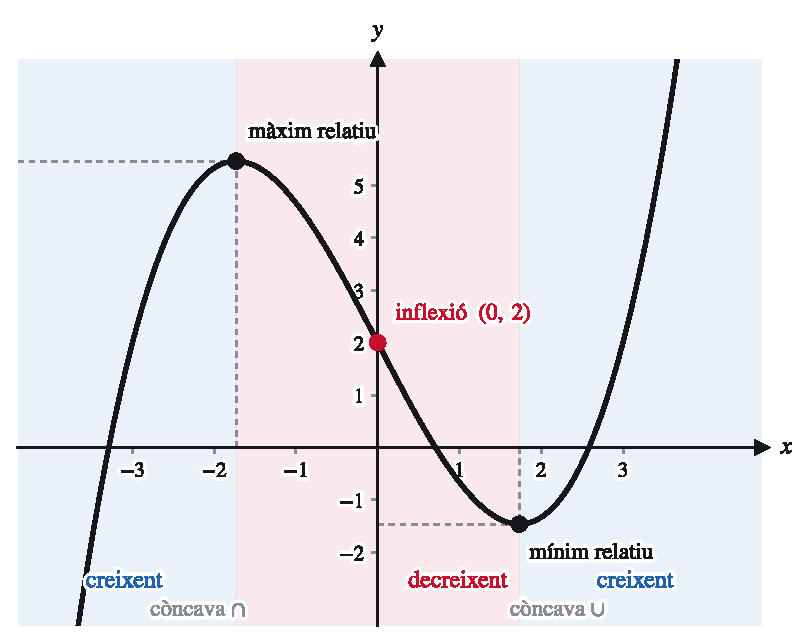
\includegraphics[width=389pt]{fig/m01_f01.pdf}
\caption{Representació dels conceptes de creixement, decreixement, màxim i mínim relatius, punt d'inflexió i concavitat per a $f(x) = \frac{x^3}{3} - 3x + 2$.}
\end{figure}

\section{Derivabilitat d'una funció en un punt}

\textbf{Definició:} Diem que una funció $y = f(x)$ és \textbf{derivable} en el punt $x = x_0$ si existeix el nombre $f'(x_0)$, derivada de la funció en aquest punt.

\textbf{Propietat:} Perquè una funció $y = f(x)$ sigui derivable en $x = x_0$, necessàriament ha de ser \textbf{contínua} en aquest punt. Si una funció presenta qualsevol tipus de discontinuïtat en $x = x_0$, no existeix $f'(x_0)$.

\section{Funció derivada}

La definició alternativa de la derivada, equivalent a la de l'apartat 3, és:

\begin{equation*}
f'(x_0) = \lim_{h\to 0} \frac{f(x_0 + h) - f(x_0)}{h}
\end{equation*}

Les regles pràctiques bàsiques de derivació, conegudes del curs anterior, són:

\begin{itemize}
\item Funció constant: $f(x) = k \Rightarrow f'(x) = 0$
\item Funció potencial: $f(x) = x^n \Rightarrow f'(x) = n \cdot x^{n-1}$, $\; n \in \mathbb{N}$
\item Funció suma: $f(x) = p(x) + q(x) \Rightarrow f'(x) = p'(x) + q'(x)$
\item Producte d'una constant per una funció: $f(x) = k \cdot g(x) \Rightarrow f'(x) = k \cdot g'(x)$
\end{itemize}

\section{Derivada de la funció composta. Regla de la cadena}

\textbf{Definició (Regla de la cadena):} Si $f(x) = g[u(x)]$, aleshores

\begin{equation}
f'(x) = g'[u(x)] \cdot u'(x)
\end{equation}

És a dir, per derivar una funció composta es deriva l'exterior (avaluat a l'interior) i es multiplica per la derivada de l'interior.

\section{Derivades successives}

Donada una funció derivable $f(x)$, podem trobar la seva funció derivada $f'(x)$. Moltes vegades, aquesta nova funció també és derivable. Les derivades d'ordre superior es defineixen de manera inductiva:

\begin{equation*}
f(x) \xrightarrow{\ \frac{d}{dx}\ } f'(x) \xrightarrow{\ \frac{d}{dx}\ } f''(x) \xrightarrow{\ \frac{d}{dx}\ } f'''(x) \xrightarrow{\ \frac{d}{dx}\ } \cdots \xrightarrow{\ \frac{d}{dx}\ } f^{(n)}(x)
\end{equation*}

on $f''(x)$ és la derivada segona, $f'''(x)$ la derivada tercera, i $f^{(n)}(x)$ la derivada enèsima de $f$.

Cal destacar alguns casos particulars:

\begin{itemize}
\item \textbf{Funcions polinòmiques:} per derivació successiva, qualsevol polinomi de grau $n$ s'anul\textperiodcentered{}la al derivar-lo $n + 1$ vegades.
\item \textbf{Funció exponencial:} les funcions del tipus $f(x) = k \cdot e^x$ són invariables respecte de la derivació; en derivar-les qualsevol nombre de vegades, s'obté sempre la mateixa funció.
\item \textbf{Funcions sinus i cosinus:} $f(x) = \sin x$ i $f(x) = \cos x$ generen una seqüència cíclica de derivades successives que es repeteix cada quatre derivacions:
\end{itemize}

\begin{equation*}
f(x) = \sin x \to f'(x) = \cos x \to f''(x) = -\sin x \to f'''(x) = -\cos x \to f^{(4)}(x) = \sin x \to \cdots
\end{equation*}

La figura il\textperiodcentered{}lustra la relació entre $\sin x$, $\cos x$ i les seves derivades:

\begin{figure}[!htbp]
\centering
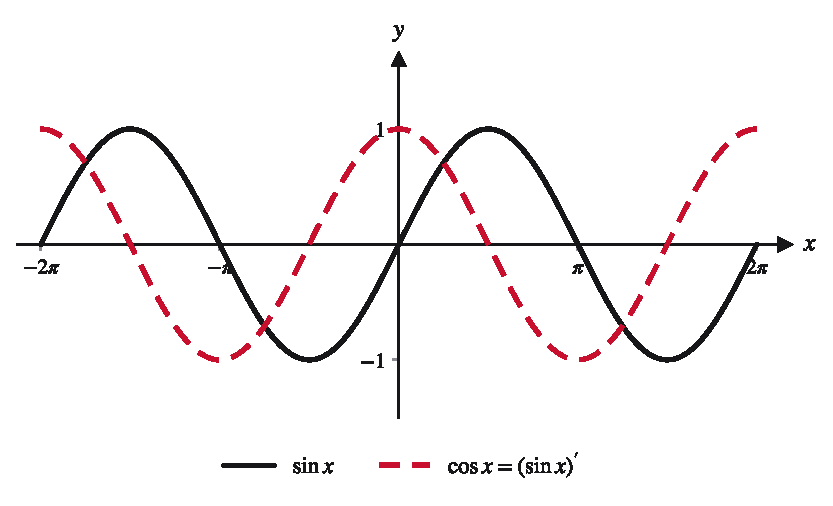
\includegraphics[width=400pt]{fig/m01_f02.pdf}
\caption{Les funcions $\sin x$ i $\cos x = (\sin x)'$ il\textperiodcentered{}lustren la seqüència cíclica de derivades successives de les funcions trigonomètriques.}
\end{figure}

\section{Taula de derivades}

La taula següent recull les derivades de les funcions elementals més habituals, on $u = u(x)$ denota una funció derivable genèrica i $u' = u'(x)$ la seva derivada.

\begin{table}[!htbp]
\centering
\renewcommand{\arraystretch}{1.75}
\begin{tabular}{lccc}
\toprule
Funció & Derivada & Funció & Derivada \\
\midrule
$k$ & $0$ & $\arctan u$ & $\displaystyle \dfrac{u'}{1+u^2}$ \\
$ax$ & $a$ & $\operatorname{arcsec} u$ & $\displaystyle \dfrac{u'}{u\sqrt{u^2-1}}$ \\
$u^n$ & $n\,u^{n-1}u'$ & $\operatorname{arccosec} u$ & $\displaystyle -\dfrac{u'}{u\sqrt{u^2-1}}$ \\
$\sqrt{u}$ & $\displaystyle \dfrac{u'}{2\sqrt{u}}$ & $\operatorname{arccotg} u$ & $\displaystyle -\dfrac{u'}{1+u^2}$ \\
$\sqrt[n]{u}$ & $\displaystyle \dfrac{u'}{n\sqrt[n]{u^{n-1}}}$ & $\sinh u$ & $\cosh u\cdot u'$ \\
$e^u$ & $e^u u'$ & $\cosh u$ & $\sinh u\cdot u'$ \\
$a^u$ & $a^u\ln a\cdot u'$ & $\tanh u$ & $\displaystyle \dfrac{u'}{\cosh^2 u}$ \\
$\ln u$ & $\displaystyle \dfrac{u'}{u}$ & $\operatorname{sech} u$ & $-\operatorname{sech} u\tanh u\cdot u'$ \\
$\log_a u$ & $\displaystyle \dfrac{u'}{u\ln a}$ & $\operatorname{cosech} u$ & $-\operatorname{cosech} u\coth u\cdot u'$ \\
$\sin u$ & $\cos u\cdot u'$ & $\coth u$ & $-\operatorname{cosech}^2 u\cdot u'$ \\
$\cos u$ & $-\sin u\cdot u'$ & $\operatorname{arcsinh} u$ & $\displaystyle \dfrac{u'}{\sqrt{u^2+1}}$ \\
$\tan u$ & $\displaystyle \dfrac{u'}{\cos^2 u}$ & $\operatorname{arccosh} u$ & $\displaystyle \dfrac{u'}{\sqrt{u^2-1}}$ \\
$\sec u$ & $\displaystyle \dfrac{u'\sin u}{\cos^2 u}$ & $\operatorname{arctanh} u$ & $\displaystyle \dfrac{u'}{1-u^2}$ \\
$\csc u$ & $\displaystyle -\dfrac{u'\cos u}{\sin^2 u}$ & $\operatorname{arcsech} u$ & $\displaystyle -\dfrac{u'}{u\sqrt{1-u^2}}$ \\
$\cot u$ & $\displaystyle -\dfrac{u'}{\sin^2 u}$ & $\operatorname{arccsch} u$ & $\displaystyle -\dfrac{u'}{u\sqrt{1+u^2}}$ \\
$\arcsin u$ & $\displaystyle \dfrac{u'}{\sqrt{1-u^2}}$ & $\operatorname{arccoth} u$ & $\displaystyle \dfrac{u'}{1-u^2}$ \\
$\arccos u$ & $\displaystyle -\dfrac{u'}{\sqrt{1-u^2}}$ &  &  \\
\bottomrule
\end{tabular}
\end{table}

\textbf{Operacions amb derivades}

\begin{table}[!htbp]
\centering
\renewcommand{\arraystretch}{1.75}
\begin{tabular}{lccc}
\toprule
Funció & Derivada & Funció & Derivada \\
\midrule
$k\cdot u$ & $k\cdot u'$ & $u+v-w$ & $u'+v'-w'$ \\
$\displaystyle \dfrac{k}{u}$ & $\displaystyle -\dfrac{k\,u'}{u^2}$ & $u\cdot v$ & $u'v+uv'$ \\
$u+v$ & $u'+v'$ & $\displaystyle \dfrac{u}{v}$ & $\displaystyle \dfrac{u'v-uv'}{v^2}$ \\
$u-v$ & $u'-v'$ &  &  \\
\bottomrule
\end{tabular}
\end{table}

\section{Complement: recta tangent i recta normal a una corba}

Geomètricament, $f'(a)$ és el \textbf{pendent de la recta tangent} a la gràfica de $f$ en el punt $P(a, f(a))$. Amb això es poden escriure les equacions de les dues rectes més demanades en un problema de derivades.

\textbf{Propietat (Recta tangent i recta normal):} si $f$ és derivable en $x=a$:

\begin{itemize}
\item \textbf{Tangent:} $\;y - f(a) = f'(a)\,(x - a)$
\item \textbf{Normal} (perpendicular a la tangent), si $f'(a)\neq 0$: $\;y - f(a) = -\dfrac{1}{f'(a)}\,(x - a)$
\end{itemize}

Si $f'(a) = 0$, la tangent és horitzontal ($y = f(a)$) i la normal és la recta vertical $x = a$.

\subsection{Mètode}

\begin{enumerate}
\item Calcular $f(a)$: això dona el punt $P(a, f(a))$.
\item Derivar $f$ i calcular el pendent $m = f'(a)$.
\item Escriure la tangent amb la fórmula punt-pendent. El pendent de la normal és $-1/m$.
\item Aïllar $y$ per donar l'equació en forma explícita.
\end{enumerate}

\subsection{Exemple 1 --- Tangent i normal en un punt}

Trobeu la tangent i la normal a $f(x) = x^2 - 3x + 2$ en $x = 3$.

\begin{itemize}
\item $f(3) = 9 - 9 + 2 = 2$, per tant $P(3, 2)$.
\item $f'(x) = 2x - 3 \Rightarrow m = f'(3) = 3$.
\item \textbf{Tangent:} $y - 2 = 3(x - 3) \Rightarrow y = 3x - 7$.
\item \textbf{Normal:} $y - 2 = -\dfrac13 (x - 3) \Rightarrow y = -\dfrac{x}{3} + 3$.
\end{itemize}

\begin{figure}[!htbp]
\centering
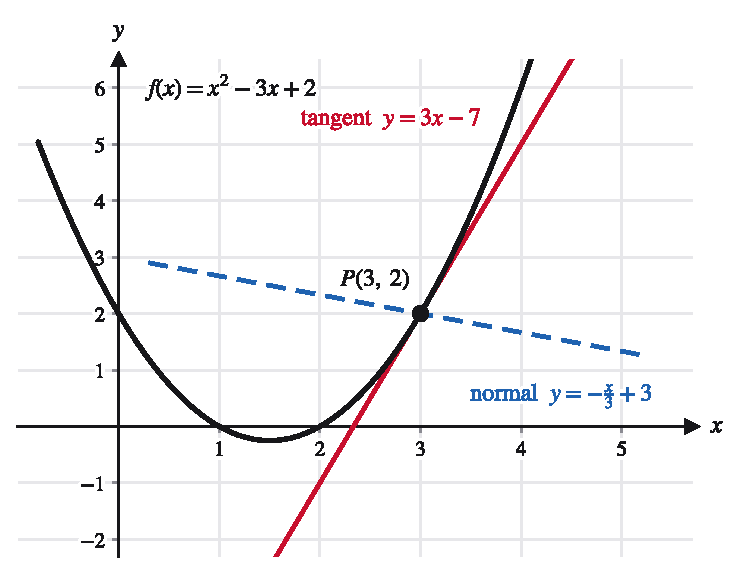
\includegraphics[width=356pt]{fig/m01_f28.pdf}
\caption{Tangent (vermell) i normal (blau, discontínua) a $f(x) = x^2 - 3x + 2$ en el punt $P(3, 2)$.}
\end{figure}

\subsection{Exemple 2 --- Tangents amb un pendent donat}

En quins punts de $f(x) = x^3 - 3x$ la tangent és paral\textperiodcentered{}lela a la recta $y = 9x + 1$?

Dues rectes són paral\textperiodcentered{}leles si tenen el mateix pendent: cal $f'(x) = 9$.

\begin{equation*}
f'(x) = 3x^2 - 3 = 9 \;\Rightarrow\; x^2 = 4 \;\Rightarrow\; x = \pm 2
\end{equation*}

\begin{itemize}
\item En $x = 2$: $f(2) = 2$, tangent $y - 2 = 9(x - 2) \Rightarrow y = 9x - 16$.
\item En $x = -2$: $f(-2) = -2$, tangent $y + 2 = 9(x + 2) \Rightarrow y = 9x + 16$.
\end{itemize}

\emph{Idea clau:} si l'enunciat dona una condició sobre la tangent (horitzontal, paral\textperiodcentered{}lela a una recta, perpendicular a una recta), s'imposa sobre $f'(x)$ i es resol l'equació.

\section{Complement: interpretació geomètrica i física de la derivada}

Quan $h$ tendeix a $0$, el punt $Q=(a+h,f(a+h))$ s'acosta a $P=(a,f(a))$ i la recta secant $PQ$ tendeix a la \textbf{recta tangent} a la corba en $P$. El pendent de la secant és la variació mitjana $\dfrac{f(a+h)-f(a)}{h}$ i el de la tangent és el seu límit, és a dir, $f'(a)$.

\begin{figure}[!htbp]
\centering
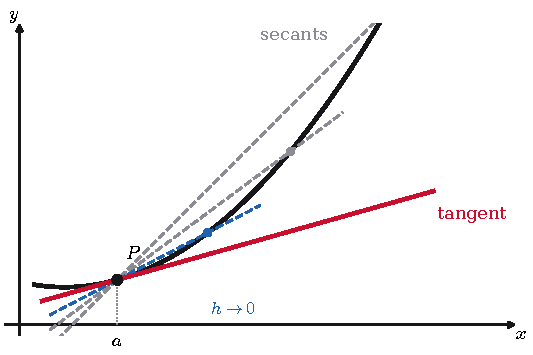
\includegraphics[width=256pt]{fig/x01_secant_tangent.pdf}
\caption{Les rectes secants (discontínues) s'aproximen a la recta tangent (vermell) quan $h\to0$: el pendent de la tangent és $f'(a)$.}
\end{figure}

La mateixa idea té una lectura física. Si $s(t)$ és la posició d'un mòbil en funció del temps, aleshores

\begin{equation*}
v(t)=s'(t)\ \text{(velocitat instantània)},\qquad a(t)=v'(t)=s''(t)\ \text{(acceleració)}.
\end{equation*}

Més generalment, $f'(a)$ mesura la \textbf{taxa de variació instantània} de $f$ en $x=a$: quant canvia $f$ per cada unitat que canvia $x$.

\emph{Exemple:} Un mòbil es mou segons $s(t)=t^3-6t^2+9t$ (metres, segons). Aleshores $v(t)=3t^2-12t+9=3(t-1)(t-3)$ i $a(t)=6t-12$. El mòbil s'atura ($v=0$) en $t=1$ s i $t=3$ s; en $t=1$ és a $s(1)=4$ m i en $t=3$ és a $s(3)=0$ m. Entre $t=1$ i $t=3$ la velocitat és negativa: retrocedeix.

\section{Complement: derivades laterals i punts de no derivabilitat}

\textbf{Definició:} Les \textbf{derivades laterals} de $f$ en $x=a$ són

\begin{equation}
f'(a^{+})=\lim_{h\to0^{+}}\frac{f(a+h)-f(a)}{h},\qquad f'(a^{-})=\lim_{h\to0^{-}}\frac{f(a+h)-f(a)}{h}.
\end{equation}

\textbf{Propietat:} $f$ és derivable en $x=a$ si i només si existeixen $f'(a^{+})$ i $f'(a^{-})$, són finites i són iguals. Aleshores $f'(a)=f'(a^{+})=f'(a^{-})$.

Una funció contínua pot deixar de ser derivable en un punt de tres maneres:

\begin{itemize}
\item \textbf{Punt angulós:} les derivades laterals existeixen però són diferents (exemple: $f(x)=|x|$ en $x=0$, amb $f'(0^-)=-1$ i $f'(0^+)=1$).
\item \textbf{Punt cuspidal:} les derivades laterals són infinites de signe oposat (exemple: $f(x)=x^{2/3}$ en $x=0$).
\item \textbf{Tangent vertical:} les dues derivades laterals són $+\infty$ (o $-\infty$) (exemple: $f(x)=\sqrt[3]{x}$ en $x=0$).
\end{itemize}

\begin{figure}[!htbp]
\centering
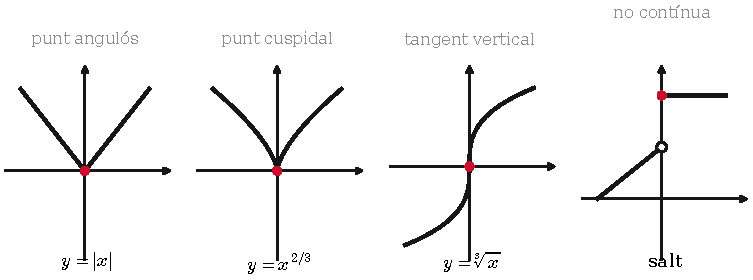
\includegraphics[width=361pt]{fig/x01_nonderiv.pdf}
\caption{Punts de no derivabilitat d'una funció contínua (punt angulós, cuspidal i tangent vertical) i funció no contínua (salt), que tampoc no és derivable.}
\end{figure}

\emph{Exemple:} Estudiem la derivabilitat de $f(x)=\begin{cases}x^2 & x\le1\\ 2x-1 & x>1\end{cases}$ en $x=1$. Contínua: $f(1^-)=1=f(1^+)$. Derivades laterals: $f'(1^-)=2x\big|_{x=1}=2$ i $f'(1^+)=2$. Coincideixen, per tant $f$ és derivable en $x=1$ amb $f'(1)=2$ (la recta $y=2x-1$ és tangent a la paràbola en $(1,1)$).

\section{Complement: demostració de les regles bàsiques de derivació}

\emph{Demostració de la derivada d'un producte.} Per a $h(x)=u(x)\,v(x)$,

\begin{equation*}
h'(x)=\lim_{h\to0}\frac{u(x+h)v(x+h)-u(x)v(x)}{h}=\lim_{h\to0}\Bigl[\frac{u(x+h)-u(x)}{h}\,v(x+h)+u(x)\,\frac{v(x+h)-v(x)}{h}\Bigr].
\end{equation*}

Com que $v$ és contínua, $v(x+h)\to v(x)$ i s'obté $(uv)'=u'v+uv'$. $\blacksquare$

\emph{Demostració de la derivada d'un quocient.} Si $q=\dfrac uv$, aleshores $u=q\,v$ i, derivant, $u'=q'v+qv'$. Aïllant, $q'=\dfrac{u'-qv'}{v}=\dfrac{u'v-uv'}{v^{2}}$. $\blacksquare$

\emph{Demostració de $(\sin x)'=\cos x$.} Amb la fórmula del sinus de la suma i els límits notables $\lim\limits_{h\to0}\frac{\sin h}{h}=1$ i $\lim\limits_{h\to0}\frac{\cos h-1}{h}=0$:

\begin{equation*}
(\sin x)'=\lim_{h\to0}\frac{\sin x\cos h+\cos x\sin h-\sin x}{h}=\sin x\cdot0+\cos x\cdot1=\cos x.\ \blacksquare
\end{equation*}

\emph{Demostració de $(x^n)'=n\,x^{n-1}$ ($n$ natural).} Pel binomi de Newton, $(x+h)^n=x^n+n\,x^{n-1}h+\binom n2x^{n-2}h^2+\dots+h^n$, de manera que $\dfrac{(x+h)^n-x^n}{h}=n\,x^{n-1}+h\,(\dots)\to n\,x^{n-1}$. $\blacksquare$

\section{Complement: derivació logarítmica, implícita, paramètrica i funció inversa}

\textbf{Derivació logarítmica.} Per a funcions del tipus $y=f(x)^{g(x)}$ es prenen logaritmes: $\ln y=g(x)\ln f(x)$, es deriva i s'aïlla $y'$:

\begin{equation*}
\frac{y'}{y}=g'\ln f+g\,\frac{f'}{f}\ \Longrightarrow\ y'=f^{\,g}\Bigl(g'\ln f+g\,\frac{f'}{f}\Bigr).
\end{equation*}

\emph{Exemple:} $y=x^{x}$ ($x>0$). $\ln y=x\ln x\Rightarrow\dfrac{y'}{y}=\ln x+1\Rightarrow y'=x^{x}(\ln x+1)$.

\textbf{Derivació implícita.} Si $y$ ve donada per una equació $F(x,y)=0$, es deriva respecte de $x$ considerant $y=y(x)$ i s'aïlla $y'$. \emph{Exemple:} a la circumferència $x^2+y^2=25$, derivant $2x+2y\,y'=0\Rightarrow y'=-\dfrac xy$. En el punt $(3,4)$ el pendent és $-\dfrac34$ i la tangent és $y-4=-\dfrac34(x-3)$, és a dir, $3x+4y=25$.

\textbf{Derivació paramètrica.} Si $x=x(t)$, $y=y(t)$, aleshores $\dfrac{dy}{dx}=\dfrac{y'(t)}{x'(t)}$. \emph{Exemple:} $x=t^2$, $y=t^3$: $\dfrac{dy}{dx}=\dfrac{3t^2}{2t}=\dfrac{3t}{2}$.

\textbf{Derivada de la funció inversa.} Si $f$ és derivable i bijectiva amb $f'(x)\neq0$, aleshores $(f^{-1})'(y)=\dfrac{1}{f'(x)}$ amb $y=f(x)$. \emph{Exemple:} $f(x)=x^3+x$ és creixent i $f(1)=2$, per tant $(f^{-1})'(2)=\dfrac{1}{f'(1)}=\dfrac14$. Aquesta regla permet deduir, per exemple, $(\arctan x)'=\dfrac{1}{1+x^2}$ a partir de $(\tan y)'=1+\tan^2y$.

\section{Complement: exemples resolts de derivades}

a) $f(x)=x^2e^{3x}$. Producte: $f'(x)=2x\,e^{3x}+x^2\cdot3e^{3x}=x\,e^{3x}(2+3x)$.

b) $f(x)=\ln(x^2+1)$. Regla de la cadena: $f'(x)=\dfrac{2x}{x^2+1}$.

c) $f(x)=\sin(x^2)\cos x$. $f'(x)=2x\cos(x^2)\cos x-\sin(x^2)\sin x$.

d) $f(x)=\dfrac{2x+1}{x^2-3}$. Quocient: $f'(x)=\dfrac{2(x^2-3)-(2x+1)2x}{(x^2-3)^2}=\dfrac{-2(x^2+x+3)}{(x^2-3)^2}$.

e) $f(x)=\sqrt{1+x^2}$. $f'(x)=\dfrac{2x}{2\sqrt{1+x^2}}=\dfrac{x}{\sqrt{1+x^2}}$.

f) $f(x)=\arctan\sqrt x$. Amb $u=\sqrt x$, $u'=\dfrac1{2\sqrt x}$: $f'(x)=\dfrac{1}{1+x}\cdot\dfrac{1}{2\sqrt x}=\dfrac{1}{2\sqrt x\,(1+x)}$.

g) $f(x)=\dfrac{\ln x}{x}$. $f'(x)=\dfrac{\frac1x\cdot x-\ln x}{x^2}=\dfrac{1-\ln x}{x^2}$.

h) $f(x)=e^{\sin x}$. $f'(x)=\cos x\,e^{\sin x}$.

\emph{Comprovació:} una bona pràctica és verificar el resultat amb un valor concret, per exemple $f(x)=x^2e^{3x}$ en $x=0$: $f'(0)=0$, coherent amb $x\,e^{3x}(2+3x)=0$.

\tema{2}{Funcions contínues i derivables}\section{Funcions contínues}

\textbf{Definició:} Una funció $f(x)$ és \textbf{contínua} en el punt $x = a$ si es verifiquen les dues condicions següents:

\begin{itemize}
\item Existeix $f(a)$; és a dir, $a$ pertany al domini de la funció.
\item Existeixen els límits laterals de $f(x)$ en el punt $a$ i coincideixen amb $f(a)$:
\end{itemize}

\begin{equation}
\lim_{x\to a^-} f(x) = \lim_{x\to a^+} f(x) = f(a)
\end{equation}

Una funció és contínua en un interval si ho és en tots i cadascun dels punts de l'interval. Podem afirmar també que totes les funcions polinòmiques són funcions contínues.

La figura il\textperiodcentered{}lustra la diferència entre una funció contínua i una de no contínua en el punt $a$:

\begin{figure}[!htbp]
\centering
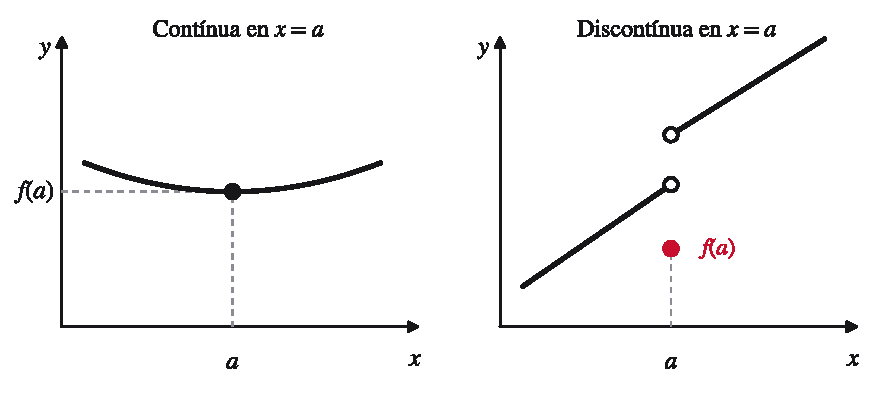
\includegraphics[width=424pt]{fig/m02_f03.pdf}
\caption{A l'esquerra, funció contínua en $x = a$: el límit coincideix amb $f(a)$. A la dreta, funció discontínua en $x = a$: els límits laterals no coincideixen amb el valor de la funció.}
\end{figure}

\section{Propietats de les funcions contínues}

\subsection{Teorema dels valors intermedis}

\textbf{Propietat (Teorema dels valors intermedis):} Sigui $f(x)$ una funció contínua en un interval tancat $[a, b]$ i $k$ un nombre tal que $f(a) \le k \le f(b)$. Aleshores, existeix almenys un punt $c \in [a, b]$ tal que $f(c) = k$.

\begin{figure}[!htbp]
\centering
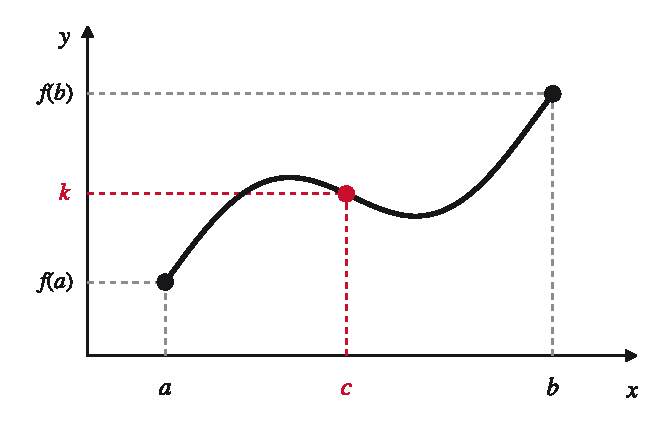
\includegraphics[width=319pt]{fig/m02_f04.pdf}
\caption{Il\textperiodcentered{}lustració del Teorema dels valors intermedis: per a tot $k$ entre $f(a)$ i $f(b)$, existeix $c \in [a, b]$ tal que $f(c) = k$.}
\end{figure}

\subsection{Teorema de Bolzano}

\textbf{Propietat (Teorema de Bolzano):} Sigui $f(x)$ una funció contínua en un interval tancat $[a, b]$ tal que $f(a)\cdot f(b) < 0$ (és a dir, $f(a)$ i $f(b)$ tenen signe diferent). Aleshores, existeix almenys un punt $c \in (a, b)$ tal que $f(c) = 0$.

\begin{figure}[!htbp]
\centering
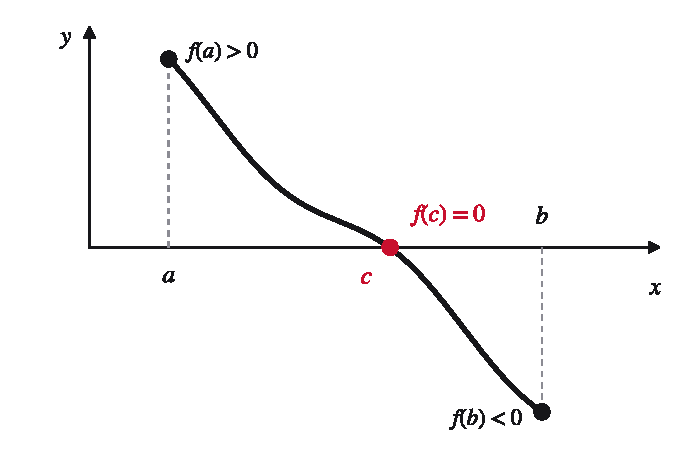
\includegraphics[width=330pt]{fig/m02_f05.pdf}
\caption{Teorema de Bolzano: $f(a) > 0$, $f(b) < 0$ i $f$ contínua en $[a, b] \Rightarrow \exists\, c \in (a, b)$ tal que $f(c) = 0$.}
\end{figure}

\section{Màxims i mínims absoluts d'una funció en un interval}

Considerem una funció $f(x)$ contínua en un interval tancat $[a, b]$. Aleshores:

\begin{itemize}
\item Existeix almenys un punt $c \in [a, b]$ en què la funció assoleix el seu \textbf{valor màxim absolut}, és a dir, $f(c) \ge f(x)$ per a tot $x \in [a, b]$.
\item Existeix almenys un punt $d \in [a, b]$ en què la funció assoleix el seu \textbf{valor mínim absolut}, és a dir, $f(d) \le f(x)$ per a tot $x \in [a, b]$.
\end{itemize}

\begin{figure}[!htbp]
\centering
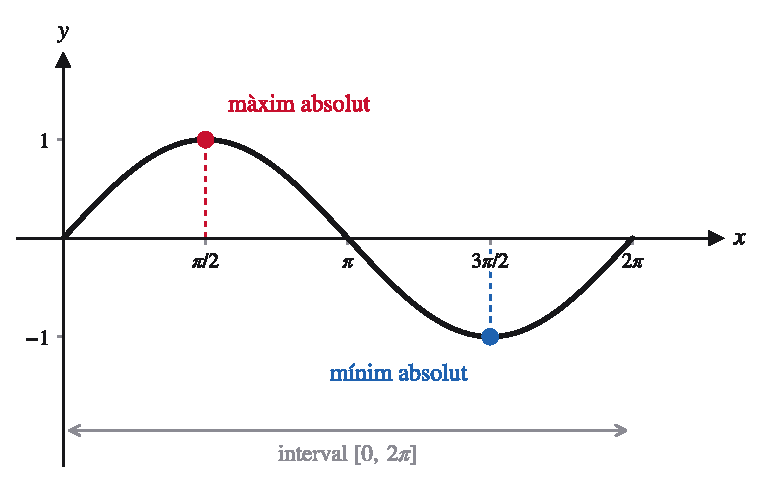
\includegraphics[width=367pt]{fig/m02_f06.pdf}
\caption{Màxim i mínim absoluts de $f(x) = \sin x$ en l'interval $[0, 2\pi]$.}
\end{figure}

\section{Funcions derivables}

\textbf{Definició:} Una funció contínua $f(x)$ és \textbf{derivable} en un punt $x = x_0$ si existeix $f'(x_0)$:

\begin{equation}
f'(x_0) = \lim_{h\to 0} \frac{f(x_0 + h) - f(x_0)}{h}
\end{equation}

Cal tenir present la relació entre continuïtat i derivabilitat:

\begin{itemize}
\item Si una funció és discontínua en un punt, no és derivable en aquell punt.
\item Una funció derivable en un punt és necessàriament contínua en aquell punt.
\end{itemize}

\subsection{Tipus de discontinuïtats}

Si $f(x)$ no és derivable en $x_0$, el límit $\displaystyle\lim_{h\to 0}\frac{f(x_0+h)-f(x_0)}{h}$ no existeix. Podem distingir tres casos:

\begin{itemize}
\item \textbf{Discontinuïtat evitable:} no existeix $f(x_0)$ i, per tant, tampoc el límit de la diferència.
\item \textbf{Discontinuïtat de salt:} el límit no existeix perquè els límits laterals a dreta i esquerra de $x_0$ no coincideixen.
\item \textbf{Discontinuïtat asimptòtica:} el límit no és numèric (un dels dos límits laterals o tots dos tendeixen a l'infinit).
\end{itemize}

La figura mostra els cinc casos possibles de no-derivabilitat o discontinuïtat en un punt $a$:

\begin{figure}[!htbp]
\centering
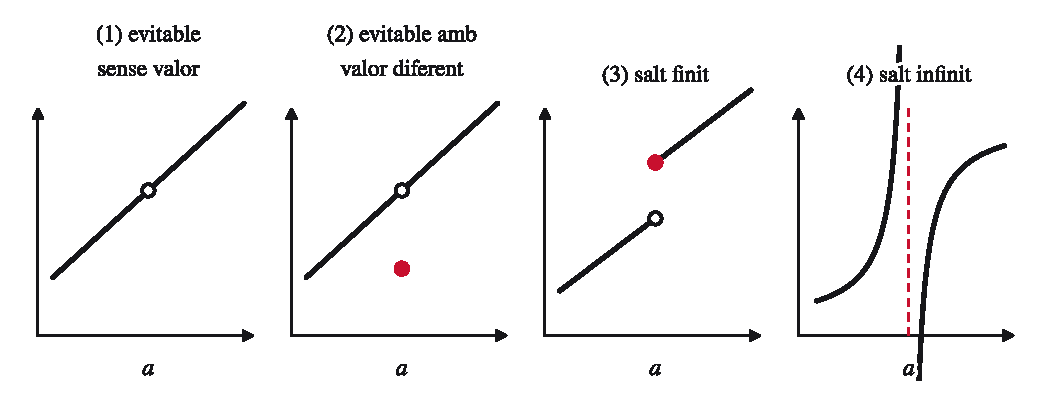
\includegraphics[width=440pt]{fig/m02_f07.pdf}
\caption{Tipus de discontinuïtats en un punt $a$: evitable sense valor (1), evitable amb valor diferent (2), salt finit (3) i salt infinit o asimptòtica (4).}
\end{figure}

\section{Propietats de les funcions derivables}

\subsection{Teorema de Rolle}

\textbf{Propietat (Teorema de Rolle):} Si $f(x)$ és contínua en $[a, b]$, derivable en $(a, b)$ i $f(a) = f(b)$, aleshores existeix almenys un punt $c \in (a, b)$ tal que $f'(c) = 0$.

\begin{figure}[!htbp]
\centering
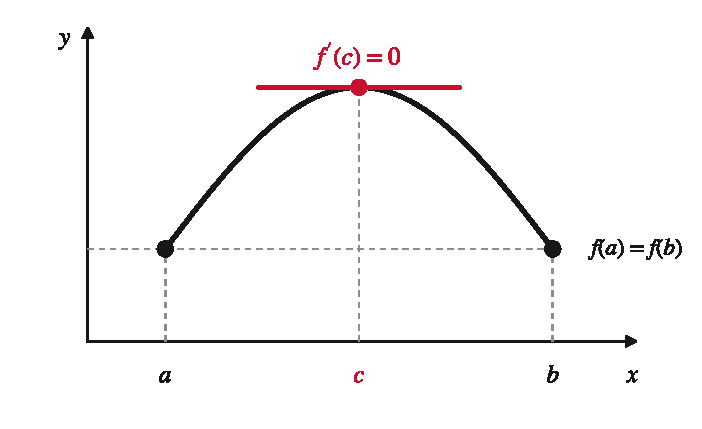
\includegraphics[width=337pt]{fig/m02_f08.pdf}
\caption{Teorema de Rolle: si $f(a) = f(b)$, existeix $c \in (a, b)$ on la tangent és horitzontal, és a dir, $f'(c) = 0$.}
\end{figure}

\subsection{Teorema del valor mitjà (Lagrange)}

\textbf{Propietat (Teorema del valor mitjà):} Si $f(x)$ és contínua en $[a, b]$ i derivable en $(a, b)$, existeix almenys un punt $c \in (a, b)$ tal que

\begin{equation}
f'(c) = \frac{f(b) - f(a)}{b - a}
\end{equation}

Geomètricament, el teorema afirma que existeix un punt $c$ on la tangent a la corba és paral\textperiodcentered{}lela a la secant que uneix $(a, f(a))$ i $(b, f(b))$.

\begin{figure}[!htbp]
\centering
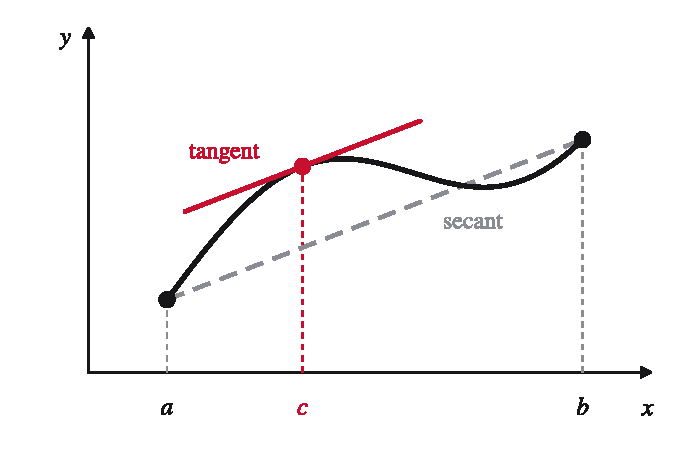
\includegraphics[width=330pt]{fig/m02_f09.pdf}
\caption{Teorema del valor mitjà: en algun punt $c \in (a, b)$, la tangent a la corba és paral\textperiodcentered{}lela a la recta secant que uneix $(a, f(a))$ i $(b, f(b))$.}
\end{figure}

\subsection{Teorema de Cauchy}

\textbf{Propietat (Teorema de Cauchy):} Si $f(x)$ i $g(x)$ són dues funcions contínues en $[a, b]$ i derivables en $(a, b)$, aleshores existeix un punt $c \in (a, b)$ tal que

\begin{equation}
\frac{f(b) - f(a)}{g(b) - g(a)} = \frac{f'(c)}{g'(c)}
\end{equation}

El teorema de Cauchy és una generalització del teorema del valor mitjà: si $g(x) = x$, aleshores $g'(c) = 1$ i es recupera exactament el resultat de Lagrange.

\section{La segona derivada}

La segona derivada d'una funció s'obté derivant la funció derivada:

\begin{equation*}
f''(x) = [f'(x)]'
\end{equation*}

La segona derivada permet caracteritzar els extrems relatius i la concavitat de la funció.

\subsection{Màxims i mínims relatius}

\begin{itemize}
\item Si $f'(x_1) = 0$ i $f''(x_1) < 0$, en $x = x_1$ hi ha un \textbf{màxim relatiu} de $f(x)$.
\item Si $f'(x_2) = 0$ i $f''(x_2) > 0$, en $x = x_2$ hi ha un \textbf{mínim relatiu} de $f(x)$.
\end{itemize}

\subsection{Concavitat d'una funció}

\begin{itemize}
\item $f(x)$ és \textbf{convexa} (còncava cap avall, $\cap$) en un interval si $f''(x) < 0$ per a tot $x$ de l'interval.
\item $f(x)$ és \textbf{còncava} (còncava cap amunt, $\cup$) en un interval si $f''(x) > 0$ per a tot $x$ de l'interval.
\end{itemize}

\subsection{Punt d'inflexió}

Si $f''(x)$ és contínua en l'interval considerat i passa de positiva a negativa (o a l'inrevés), necessàriament existirà un punt en què $f''(x) = 0$. En aquest punt canvia la concavitat de la gràfica i s'anomena \textbf{punt d'inflexió}.

\begin{figure}[!htbp]
\centering
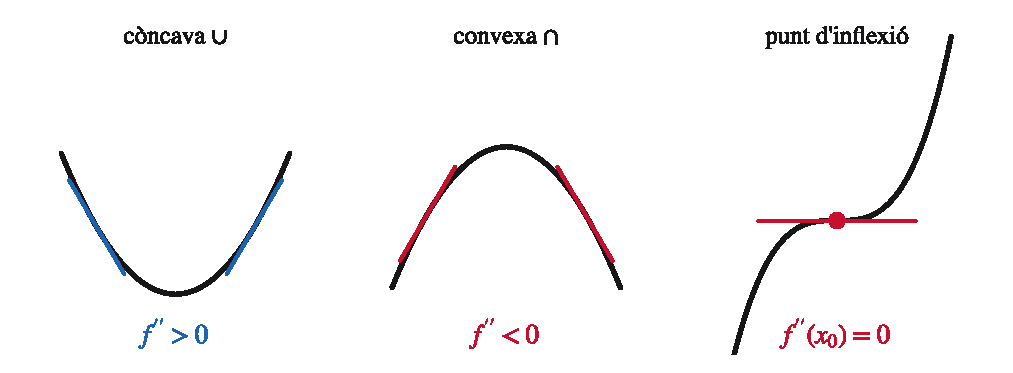
\includegraphics[width=440pt]{fig/m02_f10.pdf}
\caption{Concavitat: còncava cap amunt ($\cup$, $f'' > 0$), convexa cap avall ($\cap$, $f'' < 0$) i punt d'inflexió on canvia la concavitat ($f''(x_0) = 0$).}
\end{figure}

\section{Càlcul de límits i la derivada. Regla de l'Hôpital}

\textbf{Propietat (Regla de l'Hôpital):} Siguin $f$ i $g$ funcions derivables en un entorn de $x_0$, amb $g'(x) \neq 0$. Si el quocient $f(x)/g(x)$ presenta una indeterminació del tipus $0/0$ o $\infty/\infty$ en $x_0$, aleshores

\begin{equation}
\lim_{x\to x_0} \frac{f(x)}{g(x)} = \lim_{x\to x_0} \frac{f'(x)}{g'(x)}
\end{equation}

sempre que el límit del costat dret existeixi.

La regla s'aplica en els casos d'indeterminació del tipus $\dfrac{0}{0}$ i $\dfrac{\infty}{\infty}$, i pot aplicar-se repetidament si el quocient de les derivades continua sent indeterminat.

En els càlculs de límits, les expressions indeterminades més habituals són:

\begin{equation*}
\frac{0}{0},\quad \frac{\infty}{\infty},\quad \infty\cdot 0,\quad 1^\infty,\quad \infty^0,\quad 0^0,\quad \infty-\infty
\end{equation*}

\emph{Observació:} les indeterminacions del tipus $\infty\cdot 0$, $1^\infty$, $\infty^0$ i $0^0$ es redueixen prèviament a una forma $0/0$ o $\infty/\infty$ (per exemple, mitjançant logaritmes o inversions) per poder aplicar la regla de l'Hôpital.

\section{Complement: càlcul de límits}

\subsection{Límits laterals i límits a l'infinit}

El límit $\displaystyle\lim_{x\to a} f(x) = L$ existeix si i només si els \textbf{límits laterals} coincideixen:

\begin{equation*}
\lim_{x\to a^-} f(x) = \lim_{x\to a^+} f(x) = L
\end{equation*}

Si el límit és $\pm\infty$, hi ha una \textbf{asímptota vertical} $x = a$. Si $\displaystyle\lim_{x\to\pm\infty} f(x) = b$, hi ha una \textbf{asímptota horitzontal} $y = b$.

Per a $x\to+\infty$, les funcions elementals es poden ordenar per ordre de creixement:

\begin{equation*}
\ln x \;\ll\; x^n \;\ll\; a^x \;\;(a>1)
\end{equation*}

És a dir, una exponencial supera qualsevol potència, i una potència supera qualsevol logaritme. Això resol molts límits $\infty/\infty$ de cop d'ull.

\subsection{Les indeterminacions i com resoldre-les}

\begin{table}[!htbp]
\centering
\renewcommand{\arraystretch}{1.75}
\begin{tabularx}{\textwidth}{l>{\raggedright\arraybackslash}X}
\toprule
Indeterminació & Com tractar-la \\
\midrule
$\displaystyle \dfrac{0}{0}$ & Factoritzar i simplificar (polinomis); multiplicar pel \textbf{conjugat} (arrels); regla de l'Hôpital \\
$\displaystyle \dfrac{\infty}{\infty}$ & Dividir per la \textbf{potència més alta} de $x$ (només comparar graus); comparar ordres de creixement; Hôpital \\
$\infty - \infty$ & Fraccions: denominador comú. Arrels: multiplicar i dividir pel \textbf{conjugat} \\
$0\cdot\infty$ & Convertir en quocient $\displaystyle \frac{0}{0}$ o $\displaystyle \frac{\infty}{\infty}$ i aplicar Hôpital \\
$1^{\infty}$ & Fórmula del nombre $e$ (vegeu a sota) \\
$0^0,\ \infty^0$ & Prendre logaritmes: $\ln L = \lim g\cdot\ln f$ \\
\bottomrule
\end{tabularx}
\end{table}

\textbf{Límits notables} (per a $x\to 0$):

\begin{equation*}
\lim_{x\to0}\frac{\sin x}{x}=1,\qquad \lim_{x\to0}\frac{1-\cos x}{x^2}=\frac12,\qquad \lim_{x\to0}\frac{e^x-1}{x}=1,\qquad \lim_{x\to0}\frac{\ln(1+x)}{x}=1
\end{equation*}

\textbf{Indeterminació $1^\infty$.} Si $\displaystyle\lim_{x\to a} f(x)=1$ i $\displaystyle\lim_{x\to a} g(x)=\pm\infty$, aleshores

\begin{equation*}
\lim_{x\to a} f(x)^{g(x)} = e^{\,\lim_{x\to a} g(x)\,\bigl(f(x)-1\bigr)}
\end{equation*}

\subsection{Exemples resolts}

\textbf{a)} $\displaystyle\lim_{x\to2}\frac{x^2-4}{x-2}\;\;\left(\tfrac00\right)$: es factoritza $x^2-4=(x-2)(x+2)$ i es simplifica:

\begin{equation*}
\lim_{x\to2}(x+2)=4
\end{equation*}

\textbf{b)} $\displaystyle\lim_{x\to0}\frac{\sqrt{x+4}-2}{x}\;\;\left(\tfrac00\right)$: es multiplica pel conjugat.

\begin{equation*}
\frac{(\sqrt{x+4}-2)(\sqrt{x+4}+2)}{x(\sqrt{x+4}+2)}=\frac{x}{x(\sqrt{x+4}+2)}=\frac{1}{\sqrt{x+4}+2}\;\longrightarrow\;\frac14
\end{equation*}

\textbf{c)} $\displaystyle\lim_{x\to+\infty}\frac{3x^2-x+1}{5x^2+2}\;\;\left(\tfrac\infty\infty\right)$: mateix grau, el límit és el quocient dels coeficients dominants: $\dfrac35$.

\emph{Regla pràctica per a quocients de polinomis en $\pm\infty$:} grau del numerador $<$ grau del denominador $\Rightarrow 0$; iguals $\Rightarrow$ quocient de coeficients; numerador de grau superior $\Rightarrow\pm\infty$.

\textbf{d)} $\displaystyle\lim_{x\to+\infty}\left(\sqrt{x^2+x}-x\right)\;\;(\infty-\infty)$:

\begin{equation*}
\frac{(\sqrt{x^2+x}-x)(\sqrt{x^2+x}+x)}{\sqrt{x^2+x}+x}=\frac{x}{\sqrt{x^2+x}+x}=\frac{1}{\sqrt{1+\frac1x}+1}\;\longrightarrow\;\frac12
\end{equation*}

\textbf{e)} $\displaystyle\lim_{x\to+\infty}\left(1+\frac2x\right)^{x}\;\;(1^\infty)$:

\begin{equation*}
e^{\lim x\left(1+\frac2x-1\right)}=e^{\lim x\cdot\frac2x}=e^2
\end{equation*}

\textbf{f)} Límits laterals amb asímptota vertical: $\displaystyle\lim_{x\to3^\pm}\frac{2x+1}{x-3}$. El numerador val $7>0$ prop de $x=3$, i el denominador és petit: positiu si $x\to3^+$ i negatiu si $x\to3^-$. Per tant

\begin{equation*}
\lim_{x\to3^+}\frac{2x+1}{x-3}=+\infty,\qquad \lim_{x\to3^-}\frac{2x+1}{x-3}=-\infty
\end{equation*}

A més, $\displaystyle\lim_{x\to\pm\infty}\frac{2x+1}{x-3}=2$: asímptota horitzontal $y=2$.

\begin{figure}[!htbp]
\centering
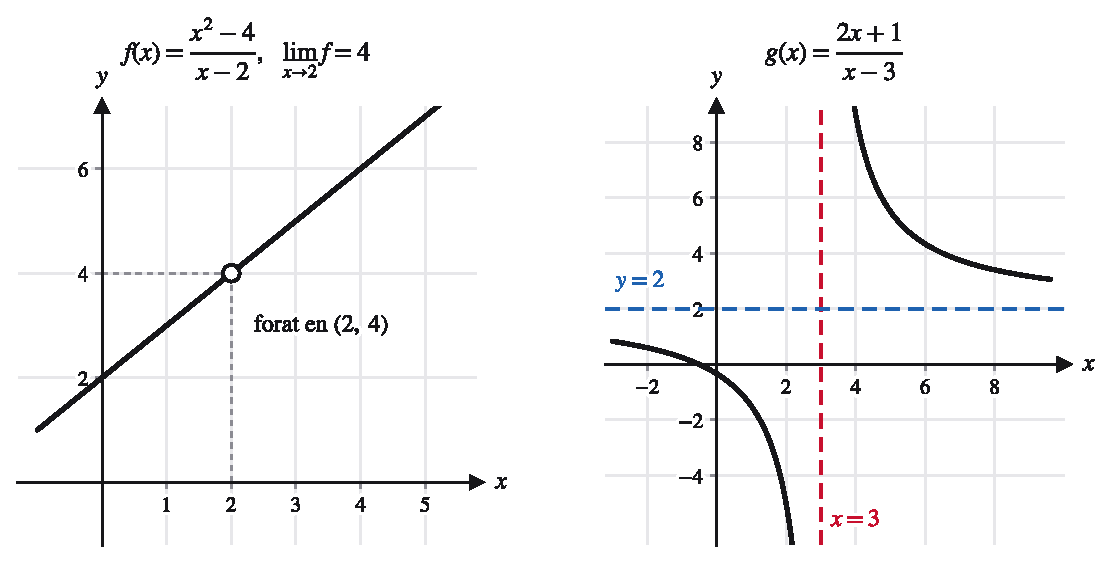
\includegraphics[width=440pt]{fig/m02_f29.pdf}
\caption{A l'esquerra, $f(x)=\dfrac{x^2-4}{x-2}$ coincideix amb $y=x+2$ excepte en $x=2$, on hi ha un forat: el límit val $4$ tot i que $f(2)$ no existeix. A la dreta, $g(x)=\dfrac{2x+1}{x-3}$ amb asímptota vertical $x=3$ i horitzontal $y=2$.}
\end{figure}

\section{Complement: funcions definides a trossos}

Una funció definida a trossos pot ser contínua i derivable en els punts on canvia l'expressió només si es compleixen unes condicions. Per a una funció

\begin{equation*}
f(x)=\begin{cases} f_1(x) & x\le a\\ f_2(x) & x>a\end{cases}
\end{equation*}

\textbf{Propietat (Continuïtat i derivabilitat en el punt de canvi):} 

\begin{itemize}
\item \textbf{Contínua en $x=a$} $\iff$ $f_1(a)=\displaystyle\lim_{x\to a^+}f_2(x)=f_2(a)$ (els dos trossos \emph{es toquen}).
\item \textbf{Derivable en $x=a$} $\iff$ és contínua \textbf{i} $f_1'(a)=f_2'(a)$ (els dos trossos \emph{s'enganxen sense angle}).
\end{itemize}

\emph{Atenció:} abans de comparar derivades cal assegurar la continuïtat. Una funció derivable sempre és contínua, però no al revés (per exemple, $f(x)=|x|$ és contínua en $0$ però no derivable: les derivades laterals valen $-1$ i $1$).

\subsection{Exemple --- Trobar paràmetres}

Determineu $a$ i $b$ perquè sigui derivable en $x=1$:

\begin{equation*}
f(x)=\begin{cases} ax^2+1 & x\le 1\\ bx-1 & x>1\end{cases}
\end{equation*}

\begin{enumerate}
\item \textbf{Continuïtat en $x=1$:} $a\cdot1^2+1=b\cdot1-1 \;\Rightarrow\; a+1=b-1 \;\Rightarrow\; b=a+2$.
\item \textbf{Derivades:} $f_1'(x)=2ax$ i $f_2'(x)=b$. En $x=1$: $2a=b$.
\item \textbf{Sistema:} $b=a+2$ i $b=2a \Rightarrow 2a=a+2 \Rightarrow a=2$, $b=4$.
\end{enumerate}

Comprovació: $f(1)=2+1=3$ pels dos costats, i les dues derivades valen $4$.

\begin{figure}[!htbp]
\centering
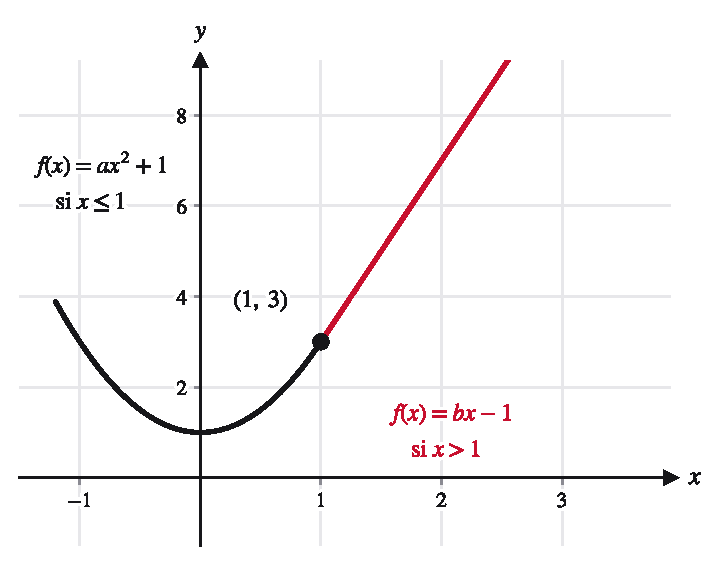
\includegraphics[width=345pt]{fig/m02_f30.pdf}
\caption{La funció a trossos amb $a=2$ i $b=4$ és contínua i derivable en $x=1$: la paràbola i la recta se uneixen en $(1, 3)$ amb el mateix pendent.}
\end{figure}

\section{Complement: demostracions dels teoremes}

Aquest apartat recull les demostracions dels teoremes d'aquest tema, perquè entenguis \textbf{d'on surten} i com s'encadenen. A la PAU normalment només cal \emph{saber aplicar-los} (comprovant les hipòtesis), però a vegades demanen explicar-ne una.

\emph{Ordre lògic:} Bolzano i Weierstrass (continuïtat) $\rightarrow$ lema de Fermat $\rightarrow$ Rolle $\rightarrow$ Lagrange $\rightarrow$ Cauchy.

\subsection{Teorema de Bolzano}

\textbf{Teorema:} si $f$ és contínua en $[a,b]$ i $f(a)\cdot f(b)<0$, existeix $c\in(a,b)$ amb $f(c)=0$.

\emph{Demostració.} Suposem $f(a)<0<f(b)$ (l'altre cas s'obté aplicant-ho a $-f$). Considerem el conjunt

\begin{equation*}
S=\{x\in[a,b]\;:\;f(x)<0\}
\end{equation*}

És no buit ($a\in S$) i està fitat superiorment per $b$; sigui $c=\sup S$. Provem que $f(c)=0$ descartant les altres dues possibilitats:

\begin{itemize}
\item \textbf{Si $f(c)<0$:} llavors $c\neq b$ (perquè $f(b)>0$). Per continuïtat, $f<0$ en un entorn de $c$, de manera que hi ha punts de $S$ més grans que $c$. Contradicció amb que $c$ és el suprem.
\item \textbf{Si $f(c)>0$:} llavors $c\neq a$. Per continuïtat, $f>0$ en un interval $(c-\delta,c]$, de manera que cap punt d'aquest interval és de $S$ i el suprem seria com a molt $c-\delta$. Contradicció.
\end{itemize}

Per tant $f(c)=0$, i com que $f(a)\neq0\neq f(b)$, $c\in(a,b)$. $\blacksquare$

\subsection{Teorema de Weierstrass (esquema)}

\textbf{Teorema:} si $f$ és contínua en $[a,b]$, existeixen $m,M$ (mínim i màxim absoluts) tals que $m\le f(x)\le M$ i $f$ pren aquests valors.

\emph{Esquema de la demostració.} \textbf{(1) $f$ està fitada.} Si no ho estigués, hi hauria una successió $x_n\in[a,b]$ amb $|f(x_n)|>n$. Com que $[a,b]$ és tancat i fitat, té una subsuccessió convergent $x_{n_k}\to x_0\in[a,b]$; per continuïtat $f(x_{n_k})\to f(x_0)$, que és un nombre finit: contradicció.

\textbf{(2) El suprem s'assoleix.} Sigui $M=\sup f$. Hi ha $x_n$ amb $f(x_n)\to M$; agafant una subsuccessió $x_{n_k}\to c\in[a,b]$, per continuïtat $f(c)=M$. Igual amb el mínim. $\blacksquare$

\subsection{Lema de Fermat}

\textbf{Lema:} si $f$ és derivable en $c$ i té un extrem relatiu en $c$ (interior a l'interval), llavors $f'(c)=0$.

\emph{Demostració.} Suposem un màxim: $f(x)\le f(c)$ prop de $c$.

\begin{itemize}
\item Per $x>c$: $\dfrac{f(x)-f(c)}{x-c}\le0$, i passant al límit, $f'(c)\le0$.
\item Per $x<c$: $\dfrac{f(x)-f(c)}{x-c}\ge0$, i passant al límit, $f'(c)\ge0$.
\end{itemize}

Com que $f'(c)$ existeix, els dos límits coincideixen: $f'(c)=0$. $\blacksquare$

\subsection{Teorema de Rolle}

\emph{Demostració.} Per Weierstrass, $f$ té màxim $M$ i mínim $m$ en $[a,b]$.

\begin{itemize}
\item \textbf{Si $M=m$}, $f$ és constant i $f'(x)=0$ en qualsevol punt de $(a,b)$.
\item \textbf{Si $M\neq m$}, com que $f(a)=f(b)$, almenys un dels dos valors (màxim o mínim) s'assoleix en un punt $c$ \textbf{interior}. Pel lema de Fermat, $f'(c)=0$. $\blacksquare$
\end{itemize}

\subsection{Teorema del valor mitjà (Lagrange)}

\emph{Demostració.} Restem de $f$ la recta secant que uneix els extrems:

\begin{equation*}
g(x)=f(x)-f(a)-\frac{f(b)-f(a)}{b-a}\,(x-a)
\end{equation*}

$g$ és contínua en $[a,b]$, derivable en $(a,b)$ i $g(a)=0=g(b)$. Per Rolle, existeix $c$ amb $g'(c)=0$, és a dir,

\begin{equation*}
f'(c)-\frac{f(b)-f(a)}{b-a}=0\;\Longrightarrow\;f'(c)=\frac{f(b)-f(a)}{b-a}.\ \blacksquare
\end{equation*}

\textbf{Conseqüència (la més usada).} Si $f'(x)>0$ en un interval, $f$ és creixent: per a $x_1<x_2$, $f(x_2)-f(x_1)=f'(c)(x_2-x_1)>0$. Igualment, si $f'(x)=0$ en tot l'interval, $f$ és constant.

\subsection{Teorema de Cauchy}

\textbf{Teorema:} si $f,g$ són contínues en $[a,b]$ i derivables en $(a,b)$, existeix $c$ amb $f'(c)\,\bigl(g(b)-g(a)\bigr)=g'(c)\,\bigl(f(b)-f(a)\bigr)$.

\emph{Demostració.} Definim $h(x)=f(x)\bigl(g(b)-g(a)\bigr)-g(x)\bigl(f(b)-f(a)\bigr)$. Es comprova que $h(a)=f(a)g(b)-g(a)f(b)=h(b)$. Per Rolle, $h'(c)=0$ per a algun $c$, que és exactament la igualtat enunciada. $\blacksquare$

\emph{Aquest teorema és la base de la regla de l'Hôpital.}

\subsection{Exemple d'aplicació d'una demostració}

\textbf{Demostra que $x^3+x-1=0$ té una única arrel real.}

\begin{itemize}
\item \emph{Existència:} $f(x)=x^3+x-1$ és contínua, $f(0)=-1<0$ i $f(1)=1>0$; per \textbf{Bolzano} hi ha una arrel a $(0,1)$.
\item \emph{Unicitat:} si hi hagués dues arrels $a<b$, com que $f(a)=f(b)=0$, per \textbf{Rolle} existiria $c$ amb $f'(c)=0$. Però $f'(x)=3x^2+1>0$ sempre: contradicció. Per tant, l'arrel és única.
\end{itemize}

\section{Complement: derivabilitat i continuïtat}

\textbf{Teorema:} Si una funció $f$ és derivable en $x=a$, aleshores és contínua en $x=a$.

\emph{Demostració.} Per a $x\neq a$ escrivim $f(x)-f(a)=\dfrac{f(x)-f(a)}{x-a}\,(x-a)$. Prenent el límit quan $x\to a$,

\begin{equation*}
\lim_{x\to a}\bigl[f(x)-f(a)\bigr]=f'(a)\cdot0=0\ \Longrightarrow\ \lim_{x\to a}f(x)=f(a).\ \blacksquare
\end{equation*}

El recíproc és fals: $f(x)=|x|$ és contínua en $x=0$ però no és derivable. Per tant, ``derivable $\Rightarrow$ contínua'', però ``contínua $\not\Rightarrow$ derivable''.

\section{Complement: aplicació dels teoremes en problemes}

Els teoremes d'aquest tema se solen aplicar per demostrar l'existència o la unicitat de solucions d'una equació.

\emph{Exemple 1 (Bolzano):} Demostrem que $x^3+x-1=0$ té alguna solució a $(0,1)$. La funció $f(x)=x^3+x-1$ és contínua a $[0,1]$, amb $f(0)=-1<0$ i $f(1)=1>0$. Pel teorema de Bolzano, existeix $c\in(0,1)$ amb $f(c)=0$.

\emph{Exemple 2 (unicitat amb Rolle):} Demostrem que aquesta solució és única. Si $f$ tingués dues arrels $c_1<c_2$, pel teorema de Rolle existiria $d\in(c_1,c_2)$ amb $f'(d)=0$. Però $f'(x)=3x^2+1>0$ per a tot $x$: contradicció. Per tant l'arrel és única.

\emph{Exemple 3 (valors intermedis):} La funció $f(x)=x^2$ pren, a $[0,3]$, tots els valors compresos entre $f(0)=0$ i $f(3)=9$; en particular $f(c)=5$ per a $c=\sqrt5\in(0,3)$.

\emph{Exemple 4 (Lagrange):} Demostrem que $|\sin b-\sin a|\le|b-a|$ per a tot $a,b$. Pel teorema del valor mitjà aplicat a $f(x)=\sin x$, existeix $c$ entre $a$ i $b$ amb $\sin b-\sin a=\cos c\,(b-a)$, i com que $|\cos c|\le1$ s'obté la desigualtat.

\emph{Exemple 5 (Weierstrass):} La funció $f(x)=\dfrac1x$ és contínua a $(0,1]$ però no té màxim absolut: el teorema de Weierstrass exigeix un interval \textbf{tancat i fitat}.

\section{Complement: funcions a trossos amb paràmetres}

Per determinar paràmetres, s'imposen les condicions de continuïtat i, si cal, de derivabilitat en els punts de canvi.

\emph{Exemple:} Trobem $a$ i $b$ perquè $f(x)=\begin{cases}x^2+a\,x & x\le1\\ 3x+b & x>1\end{cases}$ sigui derivable en $x=1$.

\begin{itemize}
\item Continuïtat: $f(1^-)=1+a$ i $f(1^+)=3+b$. Cal $1+a=3+b$.
\item Derivabilitat: $f'(1^-)=2+a$ i $f'(1^+)=3$. Cal $2+a=3$, és a dir, $a=1$.
\end{itemize}

De la primera, $b=a-2=-1$. Per tant $a=1$ i $b=-1$.

\emph{Exemple (valor absolut):} $f(x)=|x^2-1|$ es pot escriure a trossos: $f(x)=x^2-1$ si $|x|\ge1$ i $f(x)=1-x^2$ si $|x|<1$. És contínua a tot $\mathbb R$, però no és derivable en $x=\pm1$: allà $f'(1^-)=-2$ i $f'(1^+)=2$ (punts angulosos).

\tema{3}{Aplicacions de la derivada}\section{Característiques d'una funció}

\subsection{Domini i recorregut}

El conjunt de tots els valors reals de la variable independent que tenen per imatge un nombre real constitueixen el \textbf{domini} de la funció, expressat com $D_f$. El conjunt de totes les imatges reals de la funció és el \textbf{recorregut} o \textbf{rang} de la funció.

\begin{table}[!htbp]
\centering
\renewcommand{\arraystretch}{1.75}
\begin{tabular}{lc}
\toprule
Funció & Domini ($D_f$) \\
\midrule
Polinòmica $P(x)$ & $\mathbb{R}$ \\
Racional $\displaystyle \dfrac{P(x)}{Q(x)}$ & $\mathbb{R} - \{x : Q(x) = 0\}$ \\
Arrel $\sqrt[n]{P(x)}$, $n$ parell & $\mathbb{R} - \{x : P(x) < 0\}$ \\
Arrel $\sqrt[n]{P(x)}$, $n$ imparell & $\mathbb{R}$ \\
Logarítmica $\log(f(x))$ & $\mathbb{R} - \{x : f(x) \le 0\}$ \\
Exponencial $e^{f(x)}$ & $D(f)$ \\
\bottomrule
\end{tabular}
\caption{domini de les principals famílies de funcions.}
\end{table}

\subsection{Simetries}

\begin{itemize}
\item Una funció és \textbf{parella} si $f(-x) = f(x)$. La seva gràfica és simètrica respecte a l'eix d'ordenades.
\item Una funció és \textbf{imparella} si $f(-x) = -f(x)$. La seva gràfica és simètrica respecte de l'origen.
\end{itemize}

\subsection{Punts de tall amb els eixos de coordenades}

\begin{itemize}
\item Tall amb l'eix $X$ $(-, 0)$: quan $f(x) = 0$.
\item Tall amb l'eix $Y$ $(0, -)$: quan $x = 0$, és a dir, $f(0)$.
\end{itemize}

\section{Asímptotes}

Definim una \textbf{asímptota} com aquella recta límit de les rectes tangents a la gràfica de la funció quan el punt de tangència tendeix a infinit. La distància entre l'asímptota i la gràfica de la funció tendeix a zero. Hi ha tres tipus d'asímptotes:

\begin{figure}[!htbp]
\centering
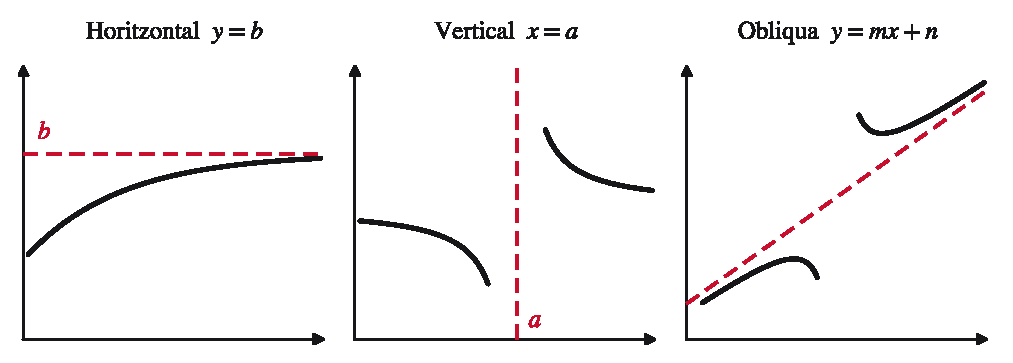
\includegraphics[width=440pt]{fig/m03_f11.pdf}
\caption{Els tres tipus d'asímptotes: horitzontal ($y = b$), vertical ($x = a$) i obliqua ($y = mx + n$).}
\end{figure}

\subsection{Asímptota vertical}

Si $f(x)$ té una discontinuïtat asimptòtica en el punt $x = a$, la recta $x = a$ és una asímptota vertical de la funció:

\begin{equation*}
\lim_{x\to a} f(x) = \infty
\end{equation*}

\subsection{Asímptota horitzontal}

Si $\displaystyle\lim_{x\to\pm\infty} f(x) = b$, la recta $y = b$ és una asímptota horitzontal. En funcions racionals $P(x)/Q(x)$:

\begin{itemize}
\item Si $\operatorname{gr}(P) > \operatorname{gr}(Q)$: no hi ha asímptota horitzontal.
\item Si $\operatorname{gr}(P) = \operatorname{gr}(Q)$: $y = \dfrac{\text{coef. principal de } P}{\text{coef. principal de } Q}$ és l'A.H.
\item Si $\operatorname{gr}(P) < \operatorname{gr}(Q)$: $y = 0$ és l'asímptota horitzontal.
\end{itemize}

\subsection{Asímptota obliqua}

L'asímptota obliqua té la forma $y = mx + n$, on:

\begin{equation*}
m = \lim_{x\to\pm\infty} \frac{f(x)}{x}, \qquad n = \lim_{x\to\pm\infty}\bigl[f(x) - mx\bigr]
\end{equation*}

En funcions racionals, existeix asímptota obliqua quan el grau del numerador supera en exactament 1 el grau del denominador (per exemple, $\dfrac{x^2+1}{x+3}$, graus 2 i 1).

\section{Optimització}

Els problemes d'\textbf{optimització} són aquells en els quals es busca el valor que fa màxima o mínima una determinada funció que correspon a la matematització d'una situació pràctica.

Per analitzar una funció, s'utilitza el signe de la derivada primera $f'(x)$ sobre la recta real, identificant els punts clau (zeros de $f'$) i determinant si corresponen a màxims, mínims o punts d'inflexió de tangent horitzontal.

\section{Complement: optimització --- mètode i exemples}

\subsection{Mètode general}

\begin{enumerate}
\item Identificar la quantitat a maximitzar o minimitzar i expressar-la com a funció $f(x)$.
\item Determinar el domini de $f$: restriccions físiques o geomètriques del problema.
\item Derivar $f'(x)$ i resoldre $f'(x) = 0$ per trobar els \textbf{punts crítics}.
\item Classificar cada punt crític:
\begin{itemize}
\item Si $f''(x_0) > 0 \Rightarrow$ mínim local.
\item Si $f''(x_0) < 0 \Rightarrow$ màxim local.
\item Comparar també els valors als extrems del domini.
\end{itemize}
\item Respondre amb les unitats correctes.
\end{enumerate}

\subsection{Exemple 1 --- Àrea màxima d'un rectangle}

Un agricultor té $80$ m de tanca per delimitar un rectangle. Quines dimensions fan l'àrea màxima?

Sigui $x$ l'amplada i $y$ l'alçada. Restricció: $2x + 2y = 80 \Rightarrow y = 40 - x$.

\begin{equation*}
A(x) = x\,(40 - x) = 40x - x^2, \qquad x \in (0, 40)
\end{equation*}

\begin{equation*}
A'(x) = 40 - 2x = 0 \Rightarrow x = 20
\end{equation*}

$A''(x) = -2 < 0 \Rightarrow$ màxim. $\;A(20) = 20\cdot 20 = 400\ \text{m}^2$.

La forma òptima és un \textbf{quadrat de $20\times 20$ m}.

\subsection{Exemple 2 --- Volum màxim d'una caixa}

D'una làmina quadrada de costat $12$ cm es retallen quadrats iguals de costat $x$ als quatre cantons i es plega. Quina $x$ maximitza el volum?

\begin{equation*}
V(x) = x\,(12 - 2x)^2, \qquad x \in (0, 6)
\end{equation*}

\begin{equation*}
V'(x) = (12-2x)^2 + x\cdot 2(12-2x)(-2) = (12-2x)\bigl[(12-2x) - 4x\bigr] = (12-2x)(12-6x)
\end{equation*}

$V'(x) = 0 \Rightarrow x = 6$ (extrem) o $x = 2$.

$V(2) = 2\cdot(8)^2 = 128\ \text{cm}^3 \Rightarrow$ \textbf{màxim}.

\subsection{Exemple 3 --- Cost mínim: una llauna cilíndrica}

Es vol fabricar una llauna cilíndrica d'un litre ($1000\ \text{cm}^3$). Quines dimensions minimitzen el material (àrea total)?

Radi $r$ i alçada $h$. Restricció del volum: $\pi r^2 h = 1000 \Rightarrow h = \dfrac{1000}{\pi r^2}$.

\begin{equation*}
A(r) = 2\pi r^2 + 2\pi r h = 2\pi r^2 + \frac{2000}{r}, \qquad r > 0
\end{equation*}

\begin{equation*}
A'(r) = 4\pi r - \frac{2000}{r^2} = 0 \;\Rightarrow\; r^3 = \frac{500}{\pi} \;\Rightarrow\; r = \sqrt[3]{\frac{500}{\pi}} \approx 5{,}42\ \text{cm}
\end{equation*}

$A''(r) = 4\pi + \dfrac{4000}{r^3} > 0 \Rightarrow$ \textbf{mínim}. Llavors $h = \dfrac{1000}{\pi r^2} \approx 10{,}84\ \text{cm}$, és a dir, $h = 2r$: la llauna òptima té l'alçada igual al diàmetre.

\section{Complement: estudi i representació gràfica d'una funció}

Representar una funció significa reunir tota la informació anterior en un dibuix. El \textbf{mètode} és sempre el mateix:

\begin{enumerate}
\item \textbf{Domini} de $f$ (quocients, arrels, logaritmes).
\item \textbf{Simetries:} parella si $f(-x)=f(x)$ (simètrica respecte de l'eix $OY$); imparella si $f(-x)=-f(x)$ (simètrica respecte de l'origen).
\item \textbf{Punts de tall:} amb l'eix $OY$, $f(0)$; amb l'eix $OX$, $f(x)=0$.
\item \textbf{Asímptotes:} verticals (punts fora del domini), horitzontals i obliqües (límits a $\pm\infty$).
\item \textbf{Monotonia i extrems:} signe de $f'$; punts crítics $f'(x)=0$.
\item \textbf{Curvatura i inflexions:} signe de $f''$; punts on $f''(x)=0$.
\item \textbf{Taula de valors} amb tots els punts singulars, i dibuix de la gràfica amb una corba suau.
\end{enumerate}

\subsection{Exemple 1 --- Un polinomi: $f(x)=x^3-3x$}

\begin{itemize}
\item \textbf{Domini:} $\mathbb{R}$. \textbf{Simetria:} $f(-x)=-f(x)$, imparella.
\item \textbf{Talls:} $f(0)=0$; $x^3-3x=x(x^2-3)=0 \Rightarrow x=0,\ x=\pm\sqrt3$.
\item \textbf{Asímptotes:} cap (és un polinomi).
\item \textbf{Monotonia:} $f'(x)=3x^2-3=3(x-1)(x+1)$, s'anul\textperiodcentered{}la en $x=\pm1$.
\end{itemize}

\begin{table}[!htbp]
\centering
\renewcommand{\arraystretch}{1.3}
\begin{tabular}{lccc}
\toprule
Interval & $(-\infty,-1)$ & $(-1,1)$ & $(1,+\infty)$ \\
\midrule
Signe de $f'$ & $+$ & $-$ & $+$ \\
$f$ & creix & decreix & creix \\
\bottomrule
\end{tabular}
\end{table}

Màxim relatiu $(-1,\,2)$ i mínim relatiu $(1,\,-2)$.

\begin{itemize}
\item \textbf{Curvatura:} $f''(x)=6x$: còncava ($\cap$) per a $x<0$, convexa ($\cup$) per a $x>0$. Inflexió en $(0,\,0)$.
\end{itemize}

\begin{figure}[!htbp]
\centering
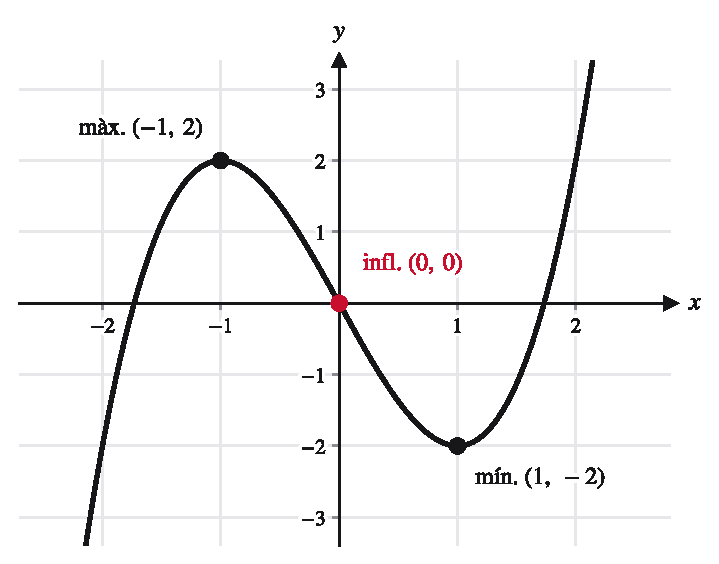
\includegraphics[width=345pt]{fig/m03_f31.pdf}
\caption{Gràfica de $f(x)=x^3-3x$ amb el màxim, el mínim i el punt d'inflexió.}
\end{figure}

\subsection{Exemple 2 --- Una funció racional: $f(x)=\dfrac{x^2}{x-1}$}

\begin{itemize}
\item \textbf{Domini:} $\mathbb{R}\setminus\{1\}$. \textbf{Simetria:} cap.
\item \textbf{Talls:} $f(0)=0$ i $x^2=0\Rightarrow x=0$ (només l'origen).
\item \textbf{Asímptota vertical:} $x=1$. $\displaystyle\lim_{x\to1^+}f=+\infty$ i $\displaystyle\lim_{x\to1^-}f=-\infty$.
\item \textbf{Asímptota obliqua:} $m=\displaystyle\lim_{x\to\infty}\frac{f(x)}{x}=1$ i $n=\displaystyle\lim_{x\to\infty}\left(\frac{x^2}{x-1}-x\right)=\lim\frac{x}{x-1}=1$. Per tant $y=x+1$.
\item \textbf{Monotonia:} $f'(x)=\dfrac{2x(x-1)-x^2}{(x-1)^2}=\dfrac{x(x-2)}{(x-1)^2}$, s'anul\textperiodcentered{}la en $x=0$ i $x=2$.
\end{itemize}

\begin{table}[!htbp]
\centering
\renewcommand{\arraystretch}{1.3}
\begin{tabular}{lcccc}
\toprule
Interval & $(-\infty,0)$ & $(0,1)$ & $(1,2)$ & $(2,+\infty)$ \\
\midrule
Signe de $f'$ & $+$ & $-$ & $-$ & $+$ \\
$f$ & creix & decreix & decreix & creix \\
\bottomrule
\end{tabular}
\end{table}

Màxim relatiu $(0,\,0)$ i mínim relatiu $(2,\,4)$.

\begin{itemize}
\item \textbf{Curvatura:} $f''(x)=\dfrac{2}{(x-1)^3}$: còncava per a $x<1$ i convexa per a $x>1$. No hi ha punts d'inflexió ($f''\neq0$ sempre).
\end{itemize}

\begin{figure}[!htbp]
\centering
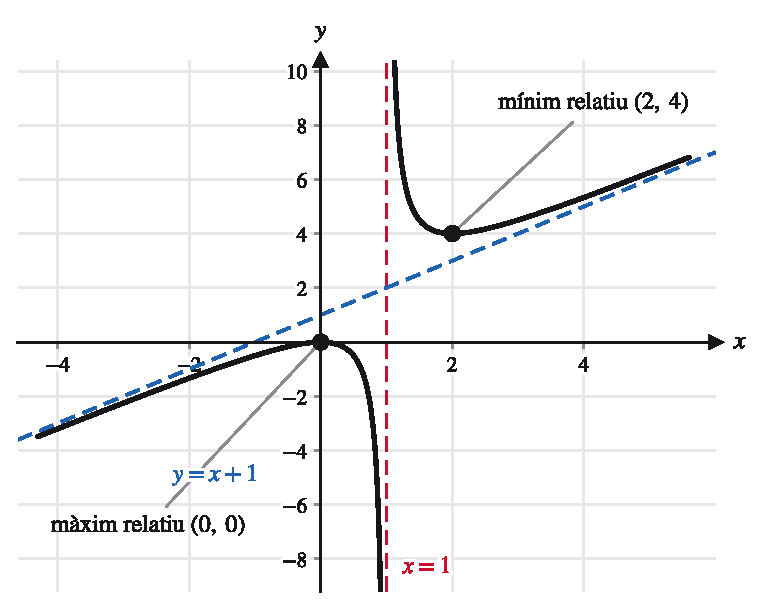
\includegraphics[width=367pt]{fig/m03_f32.pdf}
\caption{Gràfica de $f(x)=\dfrac{x^2}{x-1}$ amb l'asímptota vertical $x=1$ (vermell) i l'obliqua $y=x+1$ (blau).}
\end{figure}

\subsection{Exemple 3 --- Amb exponencial: $f(x)=x\,e^{-x}$}

\begin{itemize}
\item \textbf{Domini:} $\mathbb{R}$. \textbf{Talls:} $f(0)=0$ i $x\,e^{-x}=0\Rightarrow x=0$.
\item \textbf{Límits:} $\displaystyle\lim_{x\to+\infty}xe^{-x}=0$ (l'exponencial guanya): asímptota horitzontal $y=0$. Per a $x\to-\infty$, $f\to-\infty$ sense asímptota.
\item \textbf{Monotonia:} $f'(x)=e^{-x}(1-x)$, s'anul\textperiodcentered{}la en $x=1$. Creix per a $x<1$ i decreix per a $x>1$: màxim en $\left(1,\,\dfrac1e\right)$.
\item \textbf{Curvatura:} $f''(x)=e^{-x}(x-2)$: còncava per a $x<2$, convexa per a $x>2$. Inflexió en $\left(2,\,\dfrac{2}{e^2}\right)$.
\end{itemize}

\begin{figure}[!htbp]
\centering
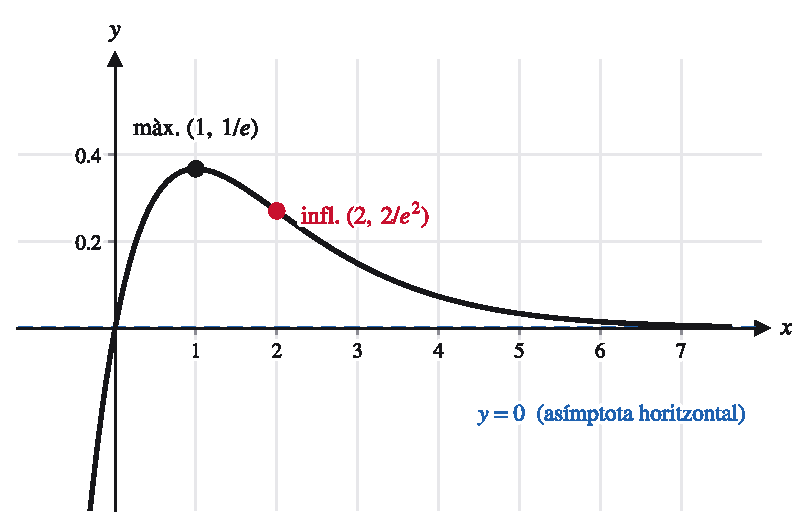
\includegraphics[width=389pt]{fig/m03_f33.pdf}
\caption{Gràfica de $f(x)=x\,e^{-x}$: màxim en $x=1$, inflexió en $x=2$ i asímptota horitzontal $y=0$ cap a $+\infty$.}
\end{figure}

\section{Complement: esquema per a l'estudi complet d'una funció}

Per representar una funció $y=f(x)$ s'aconsella seguir sempre aquest ordre:

\begin{enumerate}
\item \textbf{Domini} i, si cal, recorregut.
\item \textbf{Simetries:} parella ($f(-x)=f(x)$), imparella ($f(-x)=-f(x)$) i periodicitat.
\item \textbf{Punts de tall} amb els eixos: $f(0)$ i les solucions de $f(x)=0$.
\item \textbf{Asímptotes:} verticals (en els punts on el límit és infinit), horitzontals i obliqües.
\item \textbf{Primera derivada:} signe de $f'$, intervals de creixement i decreixement, extrems relatius.
\item \textbf{Segona derivada:} signe de $f''$, intervals de concavitat i punts d'inflexió.
\item \textbf{Taula resum} amb tots els punts notables i \textbf{gràfica} final.
\end{enumerate}

\section{Complement: més problemes d'optimització}

\emph{Exemple 4 --- Punt d'una corba més proper a un punt donat:} Trobem el punt de la paràbola $y=x^2$ més proper a $A=\bigl(0,\tfrac32\bigr)$. Es minimitza el quadrat de la distància (el mateix punt minimitza la distància i s'evita l'arrel):

\begin{equation*}
d^2(x)=x^2+\Bigl(x^2-\frac32\Bigr)^2=x^4-2x^2+\frac94.
\end{equation*}

Aleshores $(d^2)'=4x^3-4x=4x(x-1)(x+1)=0\Rightarrow x=0,\pm1$. Com que $d^2(0)=\tfrac94$ i $d^2(\pm1)=\tfrac54$, els mínims són els punts $(\pm1,1)$, a distància $d=\dfrac{\sqrt5}{2}\approx1{,}12$. ($x=0$ és un màxim relatiu.)

\emph{Exemple 5 --- Plantilla amb talls:} Per construir la caixa de l'exemple 2 es retallen quadrats de costat $x$ a les quatre cantonades de la làmina de 12 cm. La figura mostra la plantilla i la caixa resultant.

\begin{figure}[!htbp]
\centering
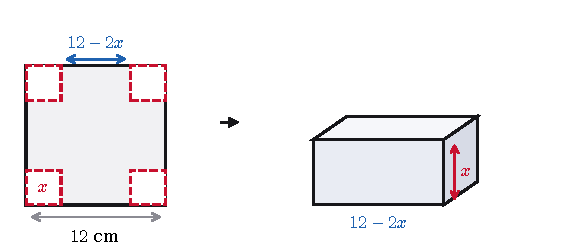
\includegraphics[width=278pt]{fig/x03_box_net.pdf}
\caption{Plantilla de la caixa: es retallen quatre quadrats de costat $x$ i es pleguen els laterals. Base $(12-2x)\times(12-2x)$ i alçada $x$.}
\end{figure}

\emph{Exemple 6 --- Rectangle inscrit en una semicircumferència:} Quin és el rectangle d'àrea màxima inscrit en una semicircumferència de radi $R$? Si el vèrtex és $(x,\sqrt{R^2-x^2})$, l'àrea és $A(x)=2x\sqrt{R^2-x^2}$. Derivant, $A'(x)=\dfrac{2(R^2-2x^2)}{\sqrt{R^2-x^2}}=0\Rightarrow x=\dfrac{R}{\sqrt2}$. Les dimensions són $R\sqrt2\times\dfrac{R}{\sqrt2}$ i l'àrea màxima val $R^2$.

\section{Complement: un altre estudi de funció --- $f(x)=\dfrac{\ln x}{x}$}

\begin{itemize}
\item \textbf{Domini:} $(0,+\infty)$. No té simetria.
\item \textbf{Talls:} amb $OX$ en $\ln x=0\Rightarrow x=1$, punt $(1,0)$. No talla $OY$.
\item \textbf{Asímptotes:} $\displaystyle\lim_{x\to0^{+}}\frac{\ln x}{x}=-\infty$: vertical $x=0$. $\displaystyle\lim_{x\to+\infty}\frac{\ln x}{x}=0$ (Hôpital): horitzontal $y=0$ (per la dreta).
\item \textbf{Primera derivada:} $f'(x)=\dfrac{1-\ln x}{x^2}$. S'anul\textperiodcentered{}la en $x=e$; $f'>0$ si $x<e$ i $f'<0$ si $x>e$. Màxim relatiu (i absolut) en $\bigl(e,\tfrac1e\bigr)\approx(2{,}72;\,0{,}37)$.
\item \textbf{Segona derivada:} $f''(x)=\dfrac{2\ln x-3}{x^3}$. S'anul\textperiodcentered{}la en $x=e^{3/2}\approx4{,}48$: $f''<0$ abans (convexa $\cap$) i $f''>0$ després (còncava $\cup$). Inflexió en $\bigl(e^{3/2},\tfrac32e^{-3/2}\bigr)\approx(4{,}48;\,0{,}33)$.
\end{itemize}

\begin{table}[!htbp]
\centering
\renewcommand{\arraystretch}{1.3}
\begin{tabular}{lccccc}
\toprule
$x$ & $(0,e)$ & $e$ & $(e,e^{3/2})$ & $e^{3/2}$ & $(e^{3/2},\infty)$ \\
\midrule
$f'$ & $+$ & $0$ & $-$ & $-$ & $-$ \\
$f''$ & $-$ & $-$ & $-$ & $0$ & $+$ \\
$f$ & creix, $\cap$ & màxim & decreix, $\cap$ & inflexió & decreix, $\cup$ \\
\bottomrule
\end{tabular}
\caption{estudi dels signes de $f'$ i $f''$ per a $f(x)=\ln x/x$.}
\end{table}

\tema{4}{Primitives}\section{Primitiva d'una funció}

\textbf{Definició:} La funció $F(x)$ és una \textbf{primitiva} de la funció $f(x)$ si es verifica $F'(x) = f(x)$.

\emph{Observació:} si $F(x)$ és una primitiva de $f(x)$, llavors $F(x) + C$ (on $C \in \mathbb{R}$ és una constant arbitrària) també ho és. Per tant, cada funció té infinites primitives, totes diferint en una constant.

\section{Integral indefinida}

Recordem la notació de Leibniz per a la derivada:

\begin{equation*}
f'(x) = \lim_{\Delta x\to 0}\frac{\Delta f(x)}{\Delta x} = \frac{df(x)}{dx}
\end{equation*}

La operació inversa a la derivació s'anomena \textbf{integració}. Si $F'(x) = f(x)$, escrivim:

\begin{equation*}
\int f(x)\,dx = F(x) + C
\end{equation*}

El símbol $\int$ s'anomena integral, la funció $f(x)$ és l'\textbf{integrand} i $C$ és la \textbf{constant d'integració}. L'expressió $\int f(x)\,dx$ s'anomena \textbf{integral indefinida} de $f(x)$.

\section{Primitives immediates}

A continuació es presenten les primitives immediates més usuals i les seves versions quasi-immediates (aplicant la regla de la cadena a l'inrevés):

\begin{table}[H]
\centering
\renewcommand{\arraystretch}{1.25}
\begin{tabularx}{\textwidth}{>{\raggedright\arraybackslash}X>{\raggedright\arraybackslash}X}
\toprule
Immediates & Quasi-immediates (amb funcions) \\
\midrule
$\displaystyle\int x^n\,dx = \dfrac{x^{n+1}}{n+1} + k$ \emph{(se suma 1 a l'exponent i es divideix pel mateix)} & $\displaystyle\int f^n(x)\,f'(x)\,dx = \dfrac{f^{n+1}(x)}{n+1} + k$ \\
$\displaystyle\int \dfrac{1}{x}\,dx = \ln\lvert x\rvert + k$ & $\displaystyle\int \dfrac{f'(x)}{f(x)}\,dx = \ln\lvert f(x)\rvert + k$ \\
$\displaystyle\int e^x\,dx = e^x + k$ \emph{(es queda igual)} & $\displaystyle\int e^{f(x)}f'(x)\,dx = e^{f(x)} + k$ \\
$\displaystyle\int a^x\,dx = \dfrac{a^x}{\ln a} + k$ & $\displaystyle\int a^{f(x)}f'(x)\,dx = \dfrac{a^{f(x)}}{\ln a} + k$ \\
$\displaystyle\int \sin x\,dx = -\cos x + k$ & $\displaystyle\int \sin(f(x))\,f'(x)\,dx = -\cos(f(x)) + k$ \\
$\displaystyle\int \cos x\,dx = \sin x + k$ & $\displaystyle\int \cos(f(x))\,f'(x)\,dx = \sin(f(x)) + k$ \\
$\displaystyle\int \dfrac{1}{\cos^2 x}\,dx = \int (1+\tan^2 x)\,dx = \tan x + k$ & $\displaystyle\int \dfrac{f'(x)}{\cos^2(f(x))}\,dx = \tan(f(x)) + k$ \\
$\displaystyle\int \dfrac{1}{\sin^2 x}\,dx = \int (1+\cot^2 x)\,dx = -\cot x + k$ & $\displaystyle\int \dfrac{f'(x)}{\sin^2(f(x))}\,dx = -\cot(f(x)) + k$ \\
$\displaystyle\int \dfrac{1}{\sqrt{1-x^2}}\,dx = \arcsin x + k$ & $\displaystyle\int \dfrac{f'(x)}{\sqrt{1-f^2(x)}}\,dx = \arcsin(f(x)) + k$ \\
$\displaystyle\int \dfrac{1}{1+x^2}\,dx = \arctan x + k$ & $\displaystyle\int \dfrac{f'(x)}{1+f^2(x)}\,dx = \arctan(f(x)) + k$ \\
\bottomrule
\end{tabularx}
\end{table}

\section{Primitives i operacions amb funcions}

\textbf{Propietat (Linealitat de la integral):} La integral és un operador lineal:

\begin{itemize}
\item $\displaystyle\int \bigl[f(x) + g(x)\bigr]dx = \int f(x)\,dx + \int g(x)\,dx$
\item $\displaystyle\int k\cdot f(x)\,dx = k\cdot\int f(x)\,dx, \quad k\in\mathbb{R}$
\end{itemize}

\section{Integració per parts}

La integració per parts és útil quan l'integrand és el producte de dues funcions de diferent naturalesa (per exemple, un polinomi i una exponencial, o un polinomi i un logaritme):

\begin{equation*}
\int u\,dv = u\cdot v - \int v\,du
\end{equation*}

que prové de la regla de la derivada d'un producte: $d(u\cdot v) = u\,dv + v\,du$.

\emph{Observació:} per triar $u$ i $dv$, una regla pràctica és la prioritat \textbf{LIATE}: \textbf{L}ogarítmiques, \textbf{I}nverses trigonomètriques, \textbf{A}lgebraiques (polinomis), \textbf{T}rigonomètriques, \textbf{E}xponencials. Es tria com a $u$ la funció que apareix primer a la llista.

\section{Integració per canvi de variable}

El canvi de variable permet simplificar integrals substituint la variable $x$ per una nova variable $t$ mitjançant $x = u(t)$:

\begin{equation*}
\frac{dx}{dt} = u'(t) \;\Rightarrow\; dx = u'(t)\,dt
\end{equation*}

\begin{equation*}
\int f(x)\,dx = \int f\bigl(u(t)\bigr)\cdot u'(t)\,dt
\end{equation*}

Un cop calculada la integral en termes de $t$, cal desfer el canvi per expressar el resultat en termes de $x$.

\section{Integració de funcions racionals}

Per integrar una funció racional $\dfrac{P(x)}{Q(x)}$, es procedeix de la manera següent:

\begin{enumerate}
\item Si el grau de $P$ és $\ge$ el grau de $Q$, es divideix i s'obté:
\end{enumerate}

\begin{equation*}
\int \frac{P(x)}{Q(x)}\,dx = \int c(x)\,dx + \int \frac{R(x)}{Q(x)}\,dx
\end{equation*}

on $c(x)$ és el quocient (un polinomi) i $R(x)$ és el residu de la divisió, amb $\operatorname{gr}(R) < \operatorname{gr}(Q)$.

\begin{enumerate}
\item La fracció pròpia $\dfrac{R(x)}{Q(x)}$ es descompon en fraccions parcials segons les arrels de $Q(x)$.
\item Cada fracció parcial s'integra de manera immediata.
\end{enumerate}

\section{Complement: com triar el mètode d'integració}

Davant d'una integral, primer s'intenta \textbf{simplificar} (expandir potències, dividir, usar identitats) i després es tria la tècnica segons la forma de l'integrand:

\begin{table}[H]
\centering
\renewcommand{\arraystretch}{1.25}
\begin{tabularx}{\textwidth}{>{\raggedright\arraybackslash}X>{\raggedright\arraybackslash}X}
\toprule
Forma de l'integrand & Tècnica \\
\midrule
Ja és una derivada coneguda, o $\dfrac{f'}{f}$, o $f'\cdot f^n$ & Primitiva immediata o quasi-immediata \\
Producte d'un polinomi per $e^x$, $\sin x$ o $\cos x$; o bé $\ln x$, $\arctan x$ & Integració \textbf{per parts} \\
Conté una arrel o una exponencial i es pot substituir una expressió per $t$ & \textbf{Canvi de variable} \\
Quocient de polinomis & \textbf{Fraccions simples} (si el grau del numerador és $\ge$ el del denominador, dividir primer) \\
$\sin^2x$, $\cos^2x$ & Identitats $\sin^2x=\dfrac{1-\cos2x}{2}$, $\cos^2x=\dfrac{1+\cos2x}{2}$ \\
\bottomrule
\end{tabularx}
\end{table}

\subsection{Integració per parts: regla pràctica}

\begin{equation*}
\int u\,dv = u\,v - \int v\,du
\end{equation*}

Per triar $u$ es pot seguir l'ordre \textbf{ALPES}: \emph{Arc} (arcsin, arctan), \emph{Logaritme}, \emph{Polinomi}, \emph{Exponencial}, \emph{Sinus/cosinus}. La funció que apareix \textbf{abans} a la llista es pren com a $u$ (es deriva) i l'altra com a $dv$ (es integra).

\emph{Exemple 1:} $\displaystyle\int x\,e^x\,dx$: $u=x,\ dv=e^xdx \Rightarrow du=dx,\ v=e^x$.

\begin{equation*}
\int x e^x dx = x e^x - \int e^x dx = (x-1)\,e^x + C
\end{equation*}

\emph{Exemple 2:} $\displaystyle\int \ln x\,dx$: $u=\ln x,\ dv=dx \Rightarrow du=\dfrac{dx}{x},\ v=x$.

\begin{equation*}
\int \ln x\,dx = x\ln x - \int dx = x\ln x - x + C
\end{equation*}

\emph{Exemple 3:} $\displaystyle\int x^2 e^x\,dx$: cal aplicar parts \textbf{dues vegades}.

\begin{equation*}
\int x^2e^xdx = x^2e^x - 2\int xe^xdx = x^2e^x - 2(x-1)e^x + C = (x^2-2x+2)\,e^x + C
\end{equation*}

\emph{Exemple 4 (cíclica):} $I=\displaystyle\int e^x\cos x\,dx$. Aplicant parts dues vegades reapareix $I$:

\begin{equation*}
I = e^x\cos x + \int e^x\sin x\,dx = e^x\cos x + e^x\sin x - I \;\Rightarrow\; I=\frac{e^x(\sin x+\cos x)}{2}+C
\end{equation*}

\subsection{Canvi de variable}

\emph{Exemple 5:} $\displaystyle\int\frac{dx}{1+\sqrt x}$. Es pren $t=\sqrt x$, és a dir, $x=t^2$ i $dx=2t\,dt$:

\begin{equation*}
\int\frac{2t}{1+t}\,dt=2\int\left(1-\frac{1}{1+t}\right)dt=2t-2\ln|1+t|+C=2\sqrt x-2\ln\left(1+\sqrt x\right)+C
\end{equation*}

\emph{Exemple 6 (quasi-immediata):} $\displaystyle\int\cos x\,\sin^2x\,dx$: com que $(\sin x)'=\cos x$, és de la forma $\int f'f^2$:

\begin{equation*}
\int\cos x\,\sin^2x\,dx=\frac{\sin^3x}{3}+C
\end{equation*}

\emph{Exemple 7:} $\displaystyle\int\frac{2x}{x^2+1}\,dx$ és de la forma $\int\frac{f'}{f}$:

\begin{equation*}
\int\frac{2x}{x^2+1}\,dx=\ln\left(x^2+1\right)+C
\end{equation*}

\subsection{Fraccions simples}

\emph{Exemple 8:} $\displaystyle\int\frac{3x+5}{(x-1)(x+3)}\,dx$. Es descompon:

\begin{equation*}
\frac{3x+5}{(x-1)(x+3)}=\frac{A}{x-1}+\frac{B}{x+3}\;\Rightarrow\;3x+5=A(x+3)+B(x-1)
\end{equation*}

Per a $x=1$: $8=4A\Rightarrow A=2$. Per a $x=-3$: $-4=-4B\Rightarrow B=1$. Llavors

\begin{equation*}
\int\frac{3x+5}{(x-1)(x+3)}\,dx=2\ln|x-1|+\ln|x+3|+C
\end{equation*}

\emph{Exemple 9:} $\displaystyle\int\frac{dx}{x^2-1}=\frac12\ln\left|\frac{x-1}{x+1}\right|+C$ (descomponent $\dfrac{1}{x^2-1}=\dfrac12\left(\dfrac{1}{x-1}-\dfrac{1}{x+1}\right)$).

\subsection{Identitats trigonomètriques}

\begin{equation*}
\int\sin^2x\,dx=\frac x2-\frac{\sin2x}{4}+C,\qquad \int\cos^2x\,dx=\frac x2+\frac{\sin2x}{4}+C
\end{equation*}

\emph{Comprovació:} sempre es pot verificar una primitiva \textbf{derivant el resultat}: ha de donar l'integrand.

\tema{5}{La integral}\section{La integral definida}

\textbf{Definició:} Donada una funció $f(x)$ contínua en un interval tancat $[a, b]$, s'anomena \textbf{integral definida} de $f(x)$ entre $a$ i $b$ el nombre

\begin{equation}
I = \int_a^b f(x)\,dx
\end{equation}

on $a$ és el límit inferior i $b$ és el límit superior d'integració.

Geomètricament, si $f(x) \ge 0$ a $[a, b]$, la integral definida representa l'àrea de la regió compresa entre la corba $y = f(x)$, l'eix $OX$ i les rectes verticals $x = a$ i $x = b$:

\begin{figure}[!htbp]
\centering
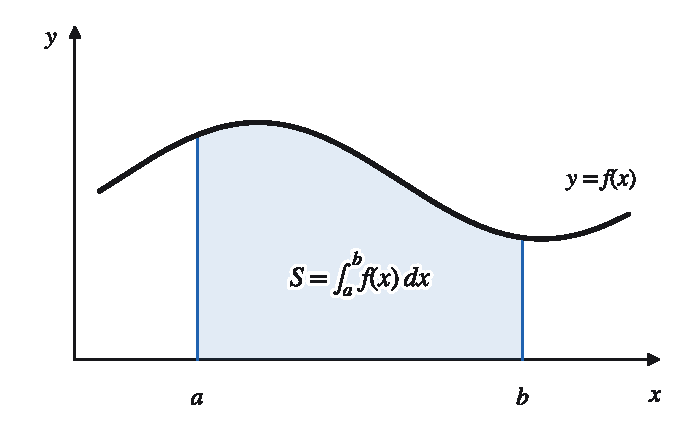
\includegraphics[width=330pt]{fig/m05_f12.pdf}
\caption{L'àrea $S$ sota la corba $f(x)$ entre $x = a$ i $x = b$ és igual a $\int_a^b f(x)\,dx$.}
\end{figure}

\section{La fórmula de Barrow. El càlcul integral}

\textbf{Propietat (Fórmula de Barrow):} Si $F(x)$ és una primitiva de $f(x)$ a $[a, b]$, aleshores

\begin{equation}
\int_a^b f(x)\,dx = \Bigl[F(x)\Bigr]_a^b = F(b) - F(a)
\end{equation}

La fórmula de Barrow connecta el càlcul de primitives (integral indefinida) amb el càlcul d'àrees (integral definida), i constitueix el \textbf{teorema fonamental del càlcul integral}.

\section{Càlcul d'àrees}

La integral definida és l'eina principal per calcular àrees de regions planes.

\subsection{Àrea compresa entre la gràfica d'una funció i l'eix OX}

Quan la funció talla l'eix $OX$ en punts intermedis $c_1, c_2, \dots$ dins de $[a, b]$, l'àrea total s'expressa com la suma del valor absolut de les integrals en cada subinterval:

\begin{equation*}
A = \left\lvert\int_a^{c_1} f(x)\,dx\right\rvert + \left\lvert\int_{c_1}^{c_2} f(x)\,dx\right\rvert + \left\lvert\int_{c_2}^{b} f(x)\,dx\right\rvert
\end{equation*}

\emph{Observació:} el valor absolut és necessari perquè la integral resulta negativa quan la funció és per sota de l'eix $OX$. Sense el valor absolut, les àrees positives i negatives es cancel\textperiodcentered{}larien parcialment.

\begin{figure}[!htbp]
\centering
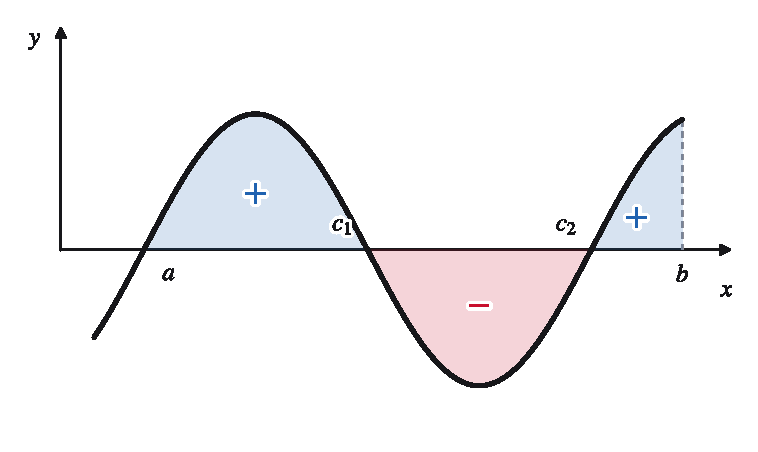
\includegraphics[width=364pt]{fig/m05_f13.pdf}
\caption{L'àrea total entre la corba i l'eix $OX$ és la suma dels valors absoluts de cada integral parcial. La zona negativa (funció per sota de l'eix) s'ha de prendre en valor absolut.}
\end{figure}

\subsection{Àrea compresa entre les gràfiques de dues funcions}

Per calcular l'àrea de la regió compresa entre dues corbes $f(x)$ i $g(x)$ en l'interval $[a, b]$:

\begin{enumerate}
\item Es troben els punts d'intersecció resolent $f(x) = g(x)$; aquests donen els límits d'integració.
\item Es calcula la diferència entre la funció superior i la inferior:
\end{enumerate}

\begin{equation*}
A = \int_a^b \bigl[g(x) - f(x)\bigr]\,dx
\end{equation*}

on $g(x) \ge f(x)$ a tot l'interval $[a, b]$.

\begin{figure}[!htbp]
\centering
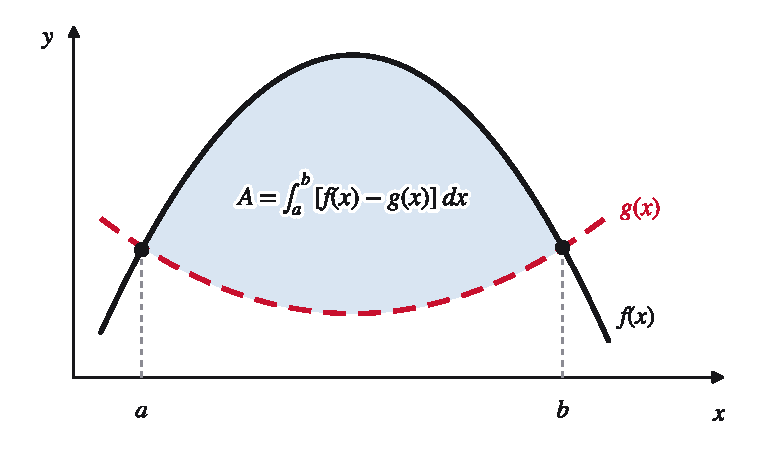
\includegraphics[width=364pt]{fig/m05_f13b.pdf}
\caption{Àrea entre les gràfiques de $f(x)$ i $g(x)$ en $[a, b]$.}
\end{figure}

\section{Complement: propietats de la integral definida}

Les propietats següents són vàlides sempre que les funcions siguin integrables als intervals indicats:

\begin{table}[!htbp]
\centering
\renewcommand{\arraystretch}{1.75}
\begin{tabular}{lc}
\toprule
Propietat & Expressió \\
\midrule
Interval degenerat & $\displaystyle \displaystyle\int_a^a f(x)\,dx = 0$ \\
Inversió dels límits & $\displaystyle \displaystyle\int_a^b f(x)\,dx = -\int_b^a f(x)\,dx$ \\
Linealitat (suma) & $\displaystyle \displaystyle\int_a^b [f(x) + g(x)]\,dx = \int_a^b f(x)\,dx + \int_a^b g(x)\,dx$ \\
Linealitat (escalar) & $\displaystyle \displaystyle\int_a^b k\,f(x)\,dx = k\int_a^b f(x)\,dx, \quad k \in \mathbb{R}$ \\
Additivitat en intervals & $\displaystyle \displaystyle\int_a^b f(x)\,dx = \int_a^c f(x)\,dx + \int_c^b f(x)\,dx, \quad a < c < b$ \\
Monotonia & Si $\displaystyle f(x) \le g(x)$ a $\displaystyle [a, b]$, llavors $\displaystyle \displaystyle\int_a^b f\,dx \le \int_a^b g\,dx$ \\
Fita de la integral & $\displaystyle \displaystyle\left\lvert\int_a^b f(x)\,dx\right\rvert \le \int_a^b |f(x)|\,dx$ \\
\bottomrule
\end{tabular}
\end{table}

\begin{figure}[!htbp]
\centering
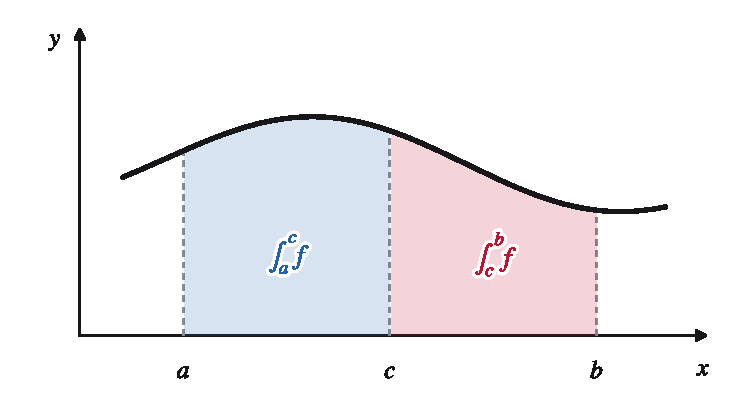
\includegraphics[width=353pt]{fig/m05_f25.pdf}
\caption{Propietat d'additivitat: $\int_a^b f = \int_a^c f + \int_c^b f$.}
\end{figure}

\section{Complement: teorema fonamental del càlcul}

\textbf{Teorema fonamental del càlcul:} si $f$ és contínua en $[a, b]$, la funció ``àrea acumulada''

\begin{equation}
F(x)=\int_a^x f(t)\,dt
\end{equation}

és derivable i $F'(x)=f(x)$ per a tot $x\in(a,b)$.

És a dir, \textbf{integrar i derivar són operacions inverses}. Si la variable apareix en un límit d'integració que és una funció $u(x)$, s'aplica la regla de la cadena:

\begin{equation*}
\frac{d}{dx}\int_a^{u(x)} f(t)\,dt=f\bigl(u(x)\bigr)\cdot u'(x)
\end{equation*}

\emph{Exemple 1:} Si $G(x)=\displaystyle\int_0^{x^2}\sin t\,dt$, llavors $G'(x)=\sin(x^2)\cdot 2x$.

\emph{Exemple 2 (amb límits):} $\displaystyle\lim_{x\to0}\frac{1}{x^2}\int_0^x\sin t\,dt$. És una indeterminació $\frac00$; per Hôpital, el numerador es deriva amb el teorema fonamental:

\begin{equation*}
\lim_{x\to0}\frac{\sin x}{2x}=\frac12
\end{equation*}

\emph{Exemple 3 (extrems):} Si $F(x)=\displaystyle\int_0^x (t^2-4)\,dt$, els punts crítics surten de $F'(x)=x^2-4=0$, és a dir, $x=\pm2$, sense calcular la integral.

\section{Complement: mètode per calcular àrees}

\subsection{Mètode}

\begin{enumerate}
\item \textbf{Fer un esquema} de les gràfiques (encara que sigui aproximat).
\item Trobar els \textbf{punts de tall} entre les corbes (o amb l'eix $OX$) resolent $f(x)=g(x)$: són els límits d'integració.
\item Veure \textbf{quina funció està per sobre} en cada tram. Si s'alternen, cal dividir en trams.
\item Calcular $\displaystyle S=\int_a^b\bigl(f_{\text{superior}}-f_{\text{inferior}}\bigr)\,dx$ en cada tram i sumar.
\item L'àrea és sempre \textbf{positiva}. \emph{Pregunta clàssica:} $\displaystyle\int_0^{2\pi}\sin x\,dx=0$, però l'àrea entre $\sin x$ i l'eix $OX$ en $[0,2\pi]$ és $2\displaystyle\int_0^{\pi}\sin x\,dx=4$.
\end{enumerate}

\subsection{Exemple 1 --- Entre una paràbola i una recta}

Àrea limitada per $f(x)=x^2$ i $g(x)=2x$.

\begin{itemize}
\item \textbf{Punts de tall:} $x^2=2x\Rightarrow x(x-2)=0\Rightarrow x=0,\ x=2$.
\item En $(0,2)$, per exemple $x=1$: $g(1)=2>f(1)=1$, així que la recta és la superior.
\end{itemize}

\begin{equation*}
S=\int_0^2\left(2x-x^2\right)dx=\left[x^2-\frac{x^3}{3}\right]_0^2=4-\frac83=\frac43\ \text{u}^2
\end{equation*}

\begin{figure}[!htbp]
\centering
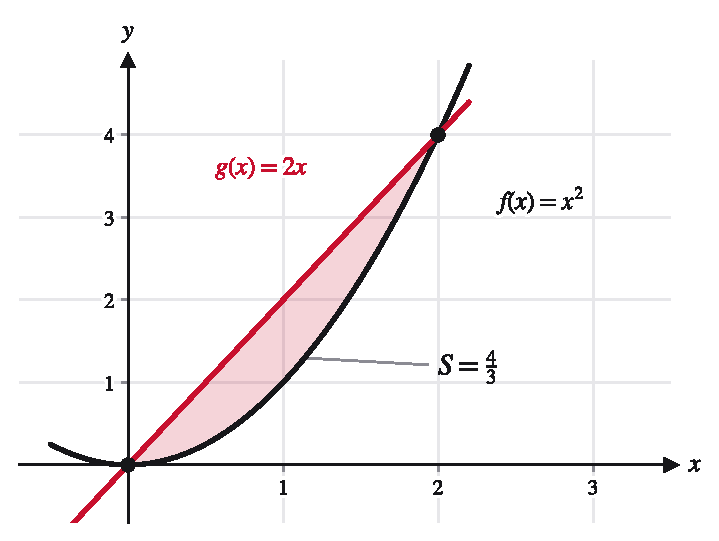
\includegraphics[width=345pt]{fig/m05_f35.pdf}
\caption{L'àrea tancada entre $f(x)=x^2$ i $g(x)=2x$ val $\frac43$.}
\end{figure}

\subsection{Exemple 2 --- Les gràfiques es creuen: $y=x^3$ i $y=x$}

\begin{itemize}
\item \textbf{Talls:} $x^3=x\Rightarrow x(x-1)(x+1)=0\Rightarrow x=-1,\,0,\,1$.
\item En $(-1,0)$: $x^3>x$ (per exemple, $x=-0{,}5$: $-0{,}125>-0{,}5$). En $(0,1)$: $x>x^3$.
\end{itemize}

\begin{equation*}
S_1=\int_{-1}^{0}(x^3-x)\,dx=\left[\frac{x^4}{4}-\frac{x^2}{2}\right]_{-1}^{0}=\frac14,\qquad S_2=\int_0^1(x-x^3)\,dx=\left[\frac{x^2}{2}-\frac{x^4}{4}\right]_0^1=\frac14
\end{equation*}

\begin{equation*}
S=S_1+S_2=\frac12\ \text{u}^2
\end{equation*}

\emph{Si es calculés $\int_{-1}^{1}(x-x^3)\,dx$ d'un sol cop, donaria $0$ per simetria: per això cal dividir en trams.}

\begin{figure}[!htbp]
\centering
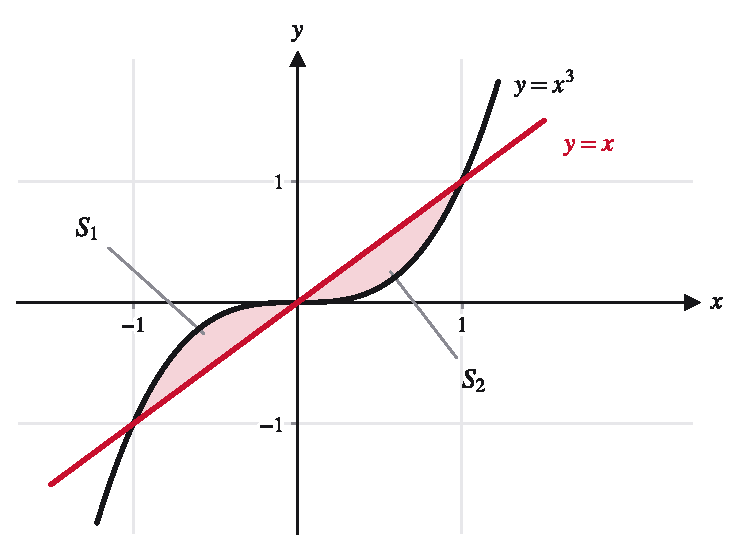
\includegraphics[width=356pt]{fig/m05_f36.pdf}
\caption{Àrea entre $y=x^3$ i $y=x$: dos trams iguals, $S_1$ i $S_2$, amb la funció superior diferent en cada un.}
\end{figure}

\section{Complement: demostracions del teorema fonamental i de la regla de Barrow}

\subsection{Teorema fonamental del càlcul}

\textbf{Teorema:} si $f$ és contínua en $[a,b]$, la funció $F(x)=\displaystyle\int_a^x f(t)\,dt$ és derivable i $F'(x)=f(x)$.

\emph{Demostració.} Per a $h>0$ petit, per la propietat d'additivitat de la integral,

\begin{equation*}
\frac{F(x+h)-F(x)}{h}=\frac1h\int_x^{x+h}f(t)\,dt
\end{equation*}

Com que $f$ és contínua en $[x,x+h]$, per Weierstrass té un mínim $m_h$ i un màxim $M_h$ en aquest interval, i l'àrea es pot acotar:

\begin{equation*}
m_h\le\frac1h\int_x^{x+h}f(t)\,dt\le M_h
\end{equation*}

Quan $h\to0$, per continuïtat, $m_h\to f(x)$ i $M_h\to f(x)$. Pel teorema de l'entrepà, el quocient tendeix a $f(x)$, és a dir, $F'(x)=f(x)$. (Per a $h<0$ es fa igual.) $\blacksquare$

\subsection{Regla de Barrow}

\textbf{Regla de Barrow:} si $f$ és contínua en $[a,b]$ i $G$ és una primitiva qualsevol de $f$, llavors

\begin{equation}
\int_a^b f(x)\,dx=G(b)-G(a)
\end{equation}

\emph{Demostració.} Siguin $F(x)=\int_a^x f$ i $G$ una primitiva. Com que $F'=f=G'$, la funció $F-G$ té derivada zero en tot l'interval i, per la conseqüència del teorema del valor mitjà, és constant: $F(x)=G(x)+C$.

Com que $F(a)=0$, resulta $C=-G(a)$. Llavors

\begin{equation*}
\int_a^b f(x)\,dx=F(b)=G(b)-G(a).\ \blacksquare
\end{equation*}

\textbf{Per què importa:} és el que permet calcular àrees amb primitives sense haver de fer límits de sumes de Riemann.

\section{Complement: sumes de Riemann i definició de la integral definida}

Per definir l'àrea sota una corba es divideix $[a,b]$ en $n$ subintervals i s'aproxima amb rectangles. La \textbf{suma inferior} $s_n$ usa el mínim de $f$ en cada subinterval i la \textbf{suma superior} $S_n$ el màxim.

\begin{figure}[!htbp]
\centering
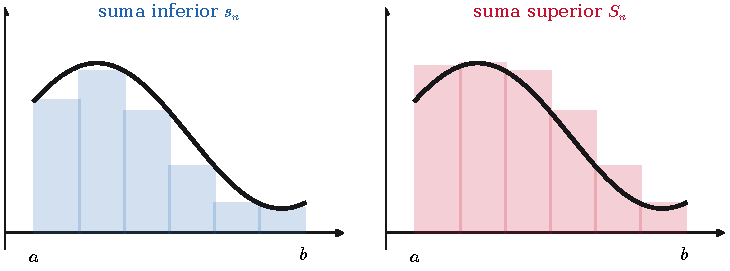
\includegraphics[width=350pt]{fig/x05_riemann.pdf}
\caption{Sumes de Riemann de $f$ en $[a,b]$ amb $n=6$ subintervals: la suma inferior $s_n$ (esquerra) i la superior $S_n$ (dreta) emmarquen l'àrea.}
\end{figure}

\textbf{Definició:} Si $f$ és contínua en $[a,b]$, les sumes inferiors i superiors tenen el mateix límit quan $n\to\infty$, i aquest límit és la \textbf{integral definida}:

\begin{equation}
\int_a^b f(x)\,dx=\lim_{n\to\infty}\sum_{i=1}^{n}f(x_i)\,\Delta x,\qquad\Delta x=\frac{b-a}{n}.
\end{equation}

\emph{Exemple:} Calculem $\displaystyle\int_0^1x^2dx$ pel límit de sumes. Amb $x_i=\dfrac in$ i $\Delta x=\dfrac1n$,

\begin{equation*}
\sum_{i=1}^{n}\frac{i^2}{n^2}\cdot\frac1n=\frac{1}{n^3}\cdot\frac{n(n+1)(2n+1)}{6}\xrightarrow[n\to\infty]{}\frac13.
\end{equation*}

El mateix resultat s'obté amb Barrow: $\left[\dfrac{x^3}{3}\right]_0^1=\dfrac13$.

\section{Complement: teorema del valor mitjà del càlcul integral}

\textbf{Teorema (del valor mitjà del càlcul integral):} Si $f$ és contínua en $[a,b]$, existeix almenys un punt $c\in[a,b]$ tal que

\begin{equation}
\int_a^b f(x)\,dx=f(c)\,(b-a).
\end{equation}

El nombre $f(c)=\dfrac{1}{b-a}\displaystyle\int_a^b f(x)\,dx$ s'anomena \textbf{valor mitjà} de $f$ en $[a,b]$: l'alçada d'un rectangle de base $b-a$ amb la mateixa àrea que la regió sota la corba.

\begin{figure}[!htbp]
\centering
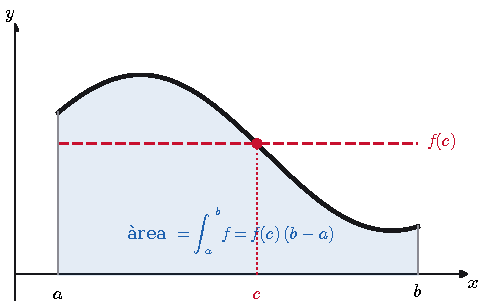
\includegraphics[width=233pt]{fig/x05_mean_value.pdf}
\caption{Teorema del valor mitjà del càlcul integral: l'àrea sota $f$ coincideix amb la del rectangle d'alçada $f(c)$ i base $b-a$.}
\end{figure}

\emph{Demostració.} Per Weierstrass, $f$ té mínim $m$ i màxim $M$ en $[a,b]$. Aleshores $m(b-a)\le\int_a^bf\le M(b-a)$, així que $\frac1{b-a}\int_a^bf$ és un valor entre $m$ i $M$; pel teorema dels valors intermedis, $f$ el pren en algun punt $c$. $\blacksquare$

\emph{Exemple:} Per a $f(x)=x^2$ en $[0,3]$: $\int_0^3x^2dx=9$, el valor mitjà és $\dfrac93=3$ i s'assoleix en $c=\sqrt3\approx1{,}73$.

\section{Complement: volum d'un cos de revolució}

Si la regió sota $y=f(x)$ entre $x=a$ i $x=b$ gira al voltant de l'eix $OX$, es genera un cos de revolució. Cada secció perpendicular a l'eix és un cercle de radi $f(x)$, amb àrea $\pi f(x)^2$; sumant-les s'obté

\begin{equation*}
V=\pi\int_a^b\bigl[f(x)\bigr]^2dx.
\end{equation*}

\begin{figure}[!htbp]
\centering
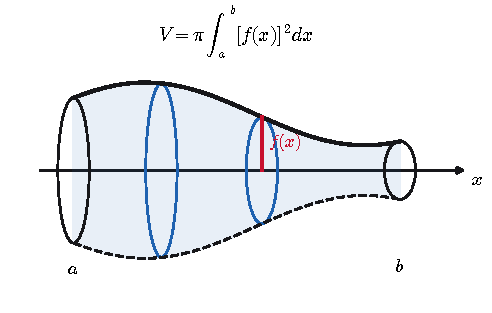
\includegraphics[width=236pt]{fig/x05_revolution.pdf}
\caption{Cos de revolució generat en girar $y=f(x)$ al voltant de l'eix $OX$: cada secció és un cercle de radi $f(x)$.}
\end{figure}

\emph{Exemples:} 

a) \emph{Con:} $y=x$ entre $0$ i $3$. $V=\pi\displaystyle\int_0^3x^2dx=\pi\cdot9=9\pi$ (coincideix amb $\frac13\pi r^2h$ per a $r=h=3$).

b) \emph{Paraboloide:} $y=\sqrt x$ entre $0$ i $4$. $V=\pi\displaystyle\int_0^4x\,dx=\pi\cdot8=8\pi$.

c) \emph{Esfera:} $y=\sqrt{r^2-x^2}$ entre $-r$ i $r$. $V=\pi\displaystyle\int_{-r}^{r}(r^2-x^2)\,dx=\pi\Bigl(2r^3-\dfrac{2r^3}{3}\Bigr)=\dfrac43\pi r^3$.

\section{Complement: més exemples d'àrees}

\emph{Exemple 1:} Àrea compresa entre $y=\sin x$ i l'eix $OX$ en $[0,2\pi]$. La funció canvia de signe en $x=\pi$, així que

\begin{equation*}
A=\int_0^{\pi}\sin x\,dx+\Bigl|\int_\pi^{2\pi}\sin x\,dx\Bigr|=2+|-2|=4.
\end{equation*}

(La integral sense separar donaria $0$: les àrees positiva i negativa es compensarien.)

\emph{Exemple 2:} Àrea entre $y=\sin x$ i $y=\cos x$ entre dues interseccions consecutives, $x=\frac\pi4$ i $x=\frac{5\pi}4$. En aquest interval $\sin x\ge\cos x$, per tant

\begin{equation*}
A=\int_{\pi/4}^{5\pi/4}(\sin x-\cos x)\,dx=\bigl[-\cos x-\sin x\bigr]_{\pi/4}^{5\pi/4}=\sqrt2+\sqrt2=2\sqrt2.
\end{equation*}

\emph{Exemple 3:} Àrea compresa entre $y=x^2$ i la recta $y=x+2$. Interseccions: $x^2=x+2\Rightarrow x=-1,\,2$. A $[-1,2]$ la recta està per sobre:

\begin{equation*}
A=\int_{-1}^{2}(x+2-x^2)\,dx=\Bigl[\frac{x^2}{2}+2x-\frac{x^3}{3}\Bigr]_{-1}^{2}=\frac{9}{2}.
\end{equation*}

% ---------------------------------------------------------------- Bloc 2
\blocitems{\begin{itemize}\item Tema 7. Matrius i determinants\item Tema 8. Sistemes d'equacions lineals\end{itemize}}
\bloc{2}{Àlgebra}{Matrius, determinants i sistemes d'equacions lineals.}
\tema{7}{Matrius i determinants}\section{Tipus de matrius}

\textbf{Definició:} Una \textbf{matriu} d'ordre $(m, n)$ és un conjunt de nombres reals disposats en $m$ files i $n$ columnes. Cada nombre rep el nom d'\textbf{element}:

\begin{equation}
A = \begin{pmatrix} a_{11} & a_{12} & a_{13} & \cdots & a_{1n} \\ a_{21} & a_{22} & a_{23} & \cdots & a_{2n} \\ \vdots & \vdots & \vdots & \ddots & \vdots \\ a_{m1} & a_{m2} & a_{m3} & \cdots & a_{mn} \end{pmatrix}
\end{equation}

Els dos subíndexs de cada element $a_{ij}$ indiquen la seva posició: $i$ és la fila i $j$ la columna. Notació alternativa: $A = (a_{ij})$ amb $i = 1, \ldots, m$ i $j = 1, \ldots, n$.

Els tipus principals de matrius són:

\begin{itemize}
\item \textbf{Matriu oposada} $(-A)$: s'obté canviant cada element pel seu oposat.
\item \textbf{Matriu transposada} $(A^t)$: resulta d'intercanviar files per columnes.
\item \textbf{Matriu identitat} $(I)$: matriu quadrada amb $a_{ij} = 1$ si $i = j$ i $a_{ij} = 0$ si $i \neq j$:
\end{itemize}

\begin{equation*}
I = \begin{pmatrix} 1 & 0 & 0 \\ 0 & 1 & 0 \\ 0 & 0 & 1 \end{pmatrix}
\end{equation*}

\begin{itemize}
\item \textbf{Matriu nul\textperiodcentered{}la:} tots els elements són $0$.
\end{itemize}

\section{Operacions amb matrius}

\subsection{Suma de matrius del mateix ordre}

Donades $A = (a_{ij})$ i $B = (b_{ij})$ del mateix ordre $(m, n)$:

\begin{equation*}
A + B = (a_{ij} + b_{ij})
\end{equation*}

Es sumen els elements que ocupen la mateixa posició.

\subsection{Producte d'un nombre real per una matriu}

Donat $k \in \mathbb{R}$ i $A = (a_{ij})$:

\begin{equation*}
k\cdot A = (k\,a_{ij})
\end{equation*}

\subsection{Producte de matrius}

Donades $A_{m\times n} = (a_{ij})$ i $B_{n\times p} = (b_{ij})$ (el nombre de columnes de $A$ ha de coincidir amb el de files de $B$), la matriu producte $C = A\cdot B$ és de tipus $m\times p$ amb:

\begin{equation*}
c_{ij} = \sum_{k=1}^{n} a_{ik}b_{kj} = a_{i1}b_{1j} + a_{i2}b_{2j} + \cdots + a_{in}b_{nj}
\end{equation*}

\emph{Observació:} en general, el producte de matrius \textbf{no és commutatiu}: $A\cdot B \neq B\cdot A$.

\subsection{Potència d'una matriu quadrada}

La potència enèsima d'una matriu quadrada $A$ és:

\begin{equation*}
A^n = A^{n-1}\cdot A, \qquad n \in \mathbb{N},\; n \ge 2
\end{equation*}

\section{Determinants}

Els determinants van associats a les matrius quadrades. El determinant de $A$ es simbolitza per $|A|$ o $\det(A)$.

\subsection{Determinant d'ordre 2}

\begin{equation*}
|A| = \begin{vmatrix} a_{11} & a_{12} \\ a_{21} & a_{22} \end{vmatrix} = a_{11}\cdot a_{22} - a_{12}\cdot a_{21}
\end{equation*}

\subsection{Determinant d'ordre 3. Regla de Sarrus}

\begin{equation*}
|A| = \begin{vmatrix} a_{11} & a_{12} & a_{13} \\ a_{21} & a_{22} & a_{23} \\ a_{31} & a_{32} & a_{33} \end{vmatrix} = a_{11}a_{22}a_{33} + a_{12}a_{23}a_{31} + a_{13}a_{21}a_{32} - a_{13}a_{22}a_{31} - a_{12}a_{21}a_{33} - a_{11}a_{23}a_{32}
\end{equation*}

La \textbf{regla de Sarrus} és un mètode gràfic per recordar aquesta fórmula: s'afegeixen les dues primeres columnes a la dreta de la matriu i s'identifiquen les sis diagonals (tres amb signe $+$ i tres amb signe $-$):

\begin{figure}[!htbp]
\centering
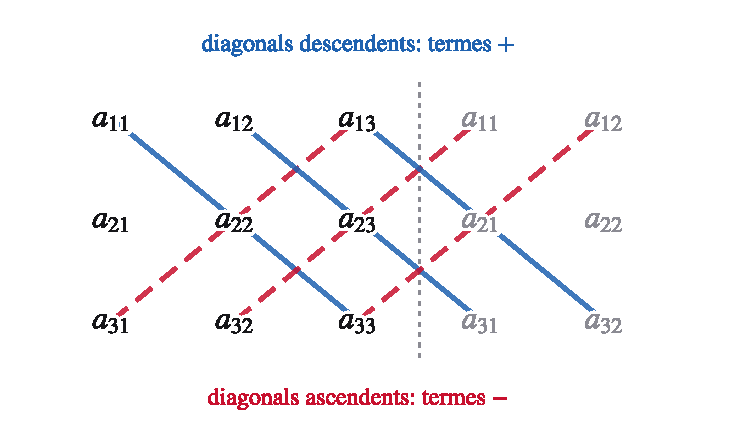
\includegraphics[width=353pt]{fig/m07_f16.pdf}
\caption{Regla de Sarrus: les tres diagonals descendents donen termes positius; les tres diagonals ascendents (en les columnes repetides), termes negatius.}
\end{figure}

\section{Adjunts d'una matriu quadrada}

D'una matriu qualsevol es poden extreure submatrius quadrades. Els determinants d'aquestes submatrius s'anomenen \textbf{menors} d'ordre $k$.

\textbf{Definició:} El \textbf{menor complementari} $M_{ij}$ és el determinant que resulta de suprimir la fila $i$ i la columna $j$ d'una matriu quadrada.

L'\textbf{adjunt} de l'element $(i, j)$ és:

\begin{equation*}
m_{ij} = (-1)^{i+j}\,M_{ij}
\end{equation*}

El signe $(-1)^{i+j}$ segueix el patró escaquer següent:

\begin{equation*}
\begin{pmatrix} + & - & + \\ - & + & - \\ + & - & + \end{pmatrix}
\end{equation*}

La \textbf{matriu adjunta} de $A$ és $A^* = (m_{ij})$, la matriu formada per tots els adjunts.

\section{Propietats dels determinants}

\begin{itemize}
\item Si una línia (fila o columna) és combinació lineal de les altres, el determinant és zero.
\item Si dues línies són iguals, el determinant és zero.
\item $\det(A) = \det(A^t)$ (el determinant és igual al de la transposada).
\item Si s'intercanvien dues línies, el determinant canvia de signe.
\item Si es multiplica una línia per $k$, el determinant queda multiplicat per $k$.
\item Un determinant amb una línia de zeros és zero.
\item $\det(I) = 1$.
\end{itemize}

\section{Rang d'una matriu}

\textbf{Definició:} El \textbf{rang} d'una matriu és l'ordre màxim dels seus menors no nuls, o equivalentment, el nombre màxim de files (o columnes) linealment independents.

Per calcular el rang d'una matriu $A$ de tipus $m\times n$:

\begin{enumerate}
\item S'identifica la dimensió màxima possible: $\operatorname{rang}(A) \le \min(m, n)$.
\item Es calcula el determinant de la submatriu quadrada d'ordre màxim:
\begin{itemize}
\item Si $\det \neq 0$: el rang és igual a aquest ordre màxim.
\item Si $\det = 0$: cal analitzar menors d'ordre inferior.
\end{itemize}
\item Es repeteix el procés reduint l'ordre fins trobar un menor no nul.
\end{enumerate}

\section{Matriu inversa}

\textbf{Definició:} La \textbf{matriu inversa} d'una matriu quadrada $A$ és la matriu $A^{-1}$ que verifica

\begin{equation}
A\cdot A^{-1} = A^{-1}\cdot A = I
\end{equation}

Una matriu que té inversa s'anomena \textbf{matriu regular}. Una matriu és regular si i només si $\det(A) \neq 0$.

La matriu inversa es calcula mitjançant la matriu adjunta transposada:

\begin{equation*}
A^{-1} = \frac{1}{|A|}\cdot(A^*)^t
\end{equation*}

\emph{Observació:} si $\det(A) = 0$, la matriu és \textbf{singular} i no té inversa.

\section{Complement: potències, equacions matricials i mètode de Gauss-Jordan}

\subsection{Potències d'una matriu: buscar el patró}

Per calcular $A^n$ amb $n$ gran no es multiplica $n$ vegades: es calculen $A^2,\,A^3,\dots$ fins veure un \textbf{patró} i es demostra per inducció.

\emph{Exemple:} $A=\begin{pmatrix}1&1\\0&1\end{pmatrix}$. Llavors $A^2=\begin{pmatrix}1&2\\0&1\end{pmatrix}$ i $A^3=\begin{pmatrix}1&3\\0&1\end{pmatrix}$, de manera que

\begin{equation*}
A^n=\begin{pmatrix}1&n\\0&1\end{pmatrix}
\end{equation*}

\emph{Demostració per inducció:} es compleix per a $n=1$; si és cert per a $n$, $A^{n+1}=A^n\cdot A=\begin{pmatrix}1&n\\0&1\end{pmatrix}\begin{pmatrix}1&1\\0&1\end{pmatrix}=\begin{pmatrix}1&n+1\\0&1\end{pmatrix}$.

\emph{Exemple (potències periòdiques):} Si $B=\begin{pmatrix}0&1\\-1&0\end{pmatrix}$, llavors $B^2=-I$, $B^3=-B$ i $B^4=I$. Les potències es repeteixen cada $4$: per a calcular $B^{2026}$ n'hi ha prou amb el residu de $2026$ entre $4$ (que és $2$), i per tant $B^{2026}=B^2=-I$.

\subsection{Equacions matricials}

Com que el producte de matrius \textbf{no és commutatiu}, cal aïllar $X$ multiplicant per la inversa \textbf{pel mateix costat} a tots dos membres:

\begin{table}[!htbp]
\centering
\renewcommand{\arraystretch}{1.3}
\begin{tabularx}{\textwidth}{l>{\raggedright\arraybackslash}X}
\toprule
Equació & Solució (si les matrius són invertibles) \\
\midrule
$A\,X=B$ & $X=A^{-1}B$ \\
$X\,A=B$ & $X=B\,A^{-1}$ \\
$A\,X+B=C$ & $X=A^{-1}(C-B)$ \\
$A\,X\,B=C$ & $X=A^{-1}\,C\,B^{-1}$ \\
$A\,X+X=B$ & $(A+I)\,X=B\Rightarrow X=(A+I)^{-1}B$ \\
\bottomrule
\end{tabularx}
\end{table}

\emph{Atenció:} en $A\,X+X=B$ no es pot treure ``factor comú'' sense la identitat: $X=I\,X$, per això surt $(A+I)$ i no $(A+1)$.

\emph{Exemple 1:} Resoleu $A\,X=B$ amb $A=\begin{pmatrix}1&2\\0&1\end{pmatrix}$ i $B=\begin{pmatrix}3&4\\1&2\end{pmatrix}$.

$|A|=1\neq0$ i $A^{-1}=\begin{pmatrix}1&-2\\0&1\end{pmatrix}$. Llavors

\begin{equation*}
X=A^{-1}B=\begin{pmatrix}1&-2\\0&1\end{pmatrix}\begin{pmatrix}3&4\\1&2\end{pmatrix}=\begin{pmatrix}1&0\\1&2\end{pmatrix}
\end{equation*}

\emph{Comprovació:} $A\,X=\begin{pmatrix}1+2&0+4\\1&2\end{pmatrix}=B$ $\checkmark$.

\emph{Exemple 2:} Resoleu $A\,X+X=B$ amb la mateixa $A$ i $B=\begin{pmatrix}2&4\\2&0\end{pmatrix}$.

$A+I=\begin{pmatrix}2&2\\0&2\end{pmatrix}$, amb $|A+I|=4$ i $(A+I)^{-1}=\dfrac14\begin{pmatrix}2&-2\\0&2\end{pmatrix}$.

\begin{equation*}
X=(A+I)^{-1}B=\frac14\begin{pmatrix}2&-2\\0&2\end{pmatrix}\begin{pmatrix}2&4\\2&0\end{pmatrix}=\frac14\begin{pmatrix}0&8\\4&0\end{pmatrix}=\begin{pmatrix}0&2\\1&0\end{pmatrix}
\end{equation*}

\emph{Exemple 3 (amb paràmetre):} Per a quins valors de $m$ té inversa $A=\begin{pmatrix}1&m\\2&3\end{pmatrix}$? Té inversa si i només si $|A|=3-2m\neq0$, és a dir, per a $m\neq\dfrac32$.

\subsection{Càlcul de la inversa pel mètode de Gauss-Jordan}

Alternativa a la fórmula dels adjunts, més còmoda per a matrius $3\times3$. S'escriu $(A\,|\,I)$ i, amb operacions entre files, es transforma $A$ en $I$; la part dreta es converteix en $A^{-1}$.

\emph{Exemple:} $A=\begin{pmatrix}2&1\\5&3\end{pmatrix}$:

\begin{equation*}
\left(\begin{array}{cc|cc}2&1&1&0\\5&3&0&1\end{array}\right)\xrightarrow{F_1/2}\left(\begin{array}{cc|cc}1&\frac12&\frac12&0\\5&3&0&1\end{array}\right)\xrightarrow{F_2-5F_1}\left(\begin{array}{cc|cc}1&\frac12&\frac12&0\\0&\frac12&-\frac52&1\end{array}\right)
\end{equation*}

\begin{equation*}
\xrightarrow{2F_2}\left(\begin{array}{cc|cc}1&\frac12&\frac12&0\\0&1&-5&2\end{array}\right)\xrightarrow{F_1-\frac12F_2}\left(\begin{array}{cc|cc}1&0&3&-1\\0&1&-5&2\end{array}\right)\;\Rightarrow\;A^{-1}=\begin{pmatrix}3&-1\\-5&2\end{pmatrix}
\end{equation*}

Si en algun moment apareix una fila de zeros a la part esquerra, $A$ \textbf{no té inversa}.

\section{Complement: interpretació geomètrica del determinant}

El valor absolut del determinant $2\times2$ és l'\textbf{àrea del paral\textperiodcentered{}lelogram} definit per les seves files (o columnes); el del determinant $3\times3$ és el \textbf{volum del paral\textperiodcentered{}lelepípede}.

\begin{figure}[!htbp]
\centering
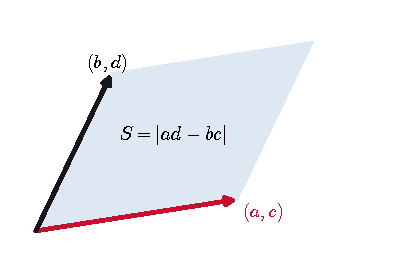
\includegraphics[width=194pt]{fig/x07_det_area.pdf}
\caption{El determinant de la matriu de columnes $(a,c)$ i $(b,d)$ és l'àrea (amb signe) del paral\textperiodcentered{}lelogram que formen.}
\end{figure}

\emph{Exemple:} Els vectors $(3,1)$ i $(1,2)$ determinen un paral\textperiodcentered{}lelogram d'àrea $\left|\begin{matrix}3&1\\1&2\end{matrix}\right|=6-1=5$.

Si $|A|=0$ els vectors són linealment dependents: el paral\textperiodcentered{}lelogram és ``pla'' (àrea $0$).

\section{Complement: propietats de la transposada i la inversa}

\begin{itemize}
\item $(A+B)^{t}=A^{t}+B^{t}$, $(kA)^{t}=kA^{t}$, $(AB)^{t}=B^{t}A^{t}$, $(A^{t})^{t}=A$.
\item $(AB)^{-1}=B^{-1}A^{-1}$, $(A^{-1})^{-1}=A$, $(A^{t})^{-1}=(A^{-1})^{t}$.
\item $|AB|=|A|\,|B|$, $|A^{t}|=|A|$, $|A^{-1}|=\dfrac1{|A|}$, $|kA|=k^{n}|A|$ si $A$ és d'ordre $n$.
\item Una matriu quadrada és \textbf{simètrica} si $A^{t}=A$ i \textbf{antisimètrica} si $A^{t}=-A$; és \textbf{ortogonal} si $A^{-1}=A^{t}$ (aleshores $|A|=\pm1$).
\item Una matriu quadrada té inversa si i només si $|A|\neq0$ si i només si $\operatorname{Rg}A=n$.
\item En general $AB\neq BA$; tampoc no es compleix $(A+B)^2=A^2+2AB+B^2$, sinó $(A+B)^2=A^2+AB+BA+B^2$.
\end{itemize}

\section{Complement: exemples resolts de determinants i inverses}

\emph{Exemple 1 --- Determinant amb paràmetre:} Per a quins valors de $a$ és invertible $A=\begin{pmatrix}1&1&1\\1&a&1\\1&1&a^2\end{pmatrix}$? Per Sarrus,

\begin{equation*}
|A|=a^3+1+1-a-a^2-1=a^3-a^2-a+1=(a-1)^2(a+1).
\end{equation*}

Així, $A$ és invertible si i només si $a\neq1$ i $a\neq-1$.

\emph{Exemple 2 --- Inversa per adjunts:} Sigui $B=\begin{pmatrix}1&0&2\\0&1&1\\1&1&0\end{pmatrix}$. Aleshores $|B|=-3\neq0$. Els adjunts són $B_{11}=-1$, $B_{12}=1$, $B_{13}=-1$, $B_{21}=2$, $B_{22}=-2$, $B_{23}=-1$, $B_{31}=-2$, $B_{32}=-1$, $B_{33}=1$. Per tant

\begin{equation*}
B^{-1}=\frac{1}{|B|}\bigl(\operatorname{Adj}B\bigr)^{t}=-\frac13\begin{pmatrix}-1&2&-2\\1&-2&-1\\-1&-1&1\end{pmatrix}=\begin{pmatrix}\frac13&-\frac23&\frac23\\-\frac13&\frac23&\frac13\\\frac13&\frac13&-\frac13\end{pmatrix}.
\end{equation*}

Es comprova que $B\,B^{-1}=I$ multiplicant.

\emph{Exemple 3 --- Rang amb paràmetre:} $\operatorname{Rg}\begin{pmatrix}1&2&3\\2&4&m\end{pmatrix}$: el menor $\begin{vmatrix}1&2\\2&4\end{vmatrix}=0$; amb la tercera columna, $\begin{vmatrix}1&3\\2&m\end{vmatrix}=m-6$. Si $m=6$, $\operatorname{Rg}=1$; si $m\neq6$, $\operatorname{Rg}=2$.

\emph{Exemple 4 --- Potència d'una matriu:} Per a $A=\begin{pmatrix}1&1\\0&1\end{pmatrix}$, $A^2=\begin{pmatrix}1&2\\0&1\end{pmatrix}$, $A^3=\begin{pmatrix}1&3\\0&1\end{pmatrix}$ i, per inducció, $A^n=\begin{pmatrix}1&n\\0&1\end{pmatrix}$.

\section{Complement: càlcul pràctic de determinants}

\subsection{Desenvolupament per una fila o columna (Laplace)}

El determinant d'una matriu quadrada és la suma dels elements d'una fila (o columna) multiplicats pels seus \textbf{adjunts}:

\begin{equation*}
|A|=\sum_{j=1}^{n}a_{ij}A_{ij},\qquad A_{ij}=(-1)^{i+j}M_{ij},
\end{equation*}

on $M_{ij}$ és el determinant que resulta d'esborrar la fila $i$ i la columna $j$. Convé triar la fila o columna amb més zeros. Els signes $(-1)^{i+j}$ formen un tauler d'escacs que comença amb $+$ a dalt a l'esquerra.

\emph{Exemple:} Calculem $\begin{vmatrix}2&0&0&1\\1&3&0&0\\0&1&1&2\\1&0&2&1\end{vmatrix}$ desenvolupant per la primera fila:

\begin{equation*}
=2\begin{vmatrix}3&0&0\\1&1&2\\0&2&1\end{vmatrix}-1\begin{vmatrix}1&3&0\\0&1&1\\1&0&2\end{vmatrix}=2\,(3\cdot(1-4))-5=-18-5=-23.
\end{equation*}

El signe de l'element $a_{14}$ és $(-1)^{1+4}=-1$.

\subsection{Triangularització (Gauss)}

Si una matriu és \textbf{triangular} (tots els elements per sota, o per sobre, de la diagonal són zero), el seu determinant és el \textbf{producte dels elements de la diagonal}. Per triangularitzar es poden fer aquestes operacions:

\begin{table}[!htbp]
\centering
\renewcommand{\arraystretch}{1.3}
\begin{tabularx}{\textwidth}{>{\raggedright\arraybackslash}X>{\raggedright\arraybackslash}X}
\toprule
Operació & Efecte sobre el determinant \\
\midrule
Intercanviar dues files (o columnes) & canvia de signe \\
Multiplicar una fila per $k\neq0$ & el determinant queda multiplicat per $k$ \\
Sumar a una fila un múltiple d'una altra ($F_i\to F_i+\lambda F_j$) & \textbf{no canvia} \\
\bottomrule
\end{tabularx}
\caption{Operacions elementals i determinant}
\end{table}

\emph{Exemple:} $\begin{vmatrix}1&2&1\\2&-1&1\\3&1&-2\end{vmatrix}$: fent $F_2\to F_2-2F_1$ i $F_3\to F_3-3F_1$ s'obté $\begin{vmatrix}1&2&1\\0&-5&-1\\0&-5&-5\end{vmatrix}$. Amb $F_3\to F_3-F_2$ queda $\begin{vmatrix}1&2&1\\0&-5&-1\\0&0&-4\end{vmatrix}=1\cdot(-5)\cdot(-4)=20$.

\subsection{Determinant de Vandermonde}

\begin{equation*}
\begin{vmatrix}1&1&1\\a&b&c\\a^{2}&b^{2}&c^{2}\end{vmatrix}=(b-a)(c-a)(c-b).
\end{equation*}

És diferent de zero si i només si $a$, $b$ i $c$ són tots diferents. Es demostra restant la primera columna a les altres dues i traient factor comú $(b-a)$ i $(c-a)$.

\section{Complement: rang d'una matriu pel mètode de Gauss}

Calcular el rang amb menors pot ser llarg. Un camí més ràpid és \textbf{escalonar} la matriu amb operacions entre files (que no canvien el rang): el rang és el nombre de \textbf{files no nul\textperiodcentered{}les} de la matriu escalonada.

\emph{Exemple:} $A=\begin{pmatrix}1&2&-1&3\\2&4&1&0\\3&6&0&3\end{pmatrix}$. Fent $F_2\to F_2-2F_1$ i $F_3\to F_3-3F_1$:

\begin{equation*}
\begin{pmatrix}1&2&-1&3\\0&0&3&-6\\0&0&3&-6\end{pmatrix}\xrightarrow{F_3\to F_3-F_2}\begin{pmatrix}1&2&-1&3\\0&0&3&-6\\0&0&0&0\end{pmatrix}.
\end{equation*}

Hi ha dues files no nul\textperiodcentered{}les: $\operatorname{Rg}A=2$.

\textbf{Propietats útils del rang.}

\begin{itemize}
\item $\operatorname{Rg}A=\operatorname{Rg}A^{t}$ i $\operatorname{Rg}(A)\le\min(m,n)$.
\item Si es fa una fila de zeros, o una fila és combinació lineal de les altres, el rang baixa.
\item Una matriu quadrada d'ordre $n$ té rang $n$ si i només si $|A|\neq0$.
\item $\operatorname{Rg}(AB)\le\min\bigl(\operatorname{Rg}A,\operatorname{Rg}B\bigr)$.
\end{itemize}

\section{Complement: equacions matricials i problemes tipus PAU}

\subsection{Equacions matricials}

Per aïllar la incògnita $X$ cal recordar que el producte \textbf{no és commutatiu}: la inversa s'ha de multiplicar pel \textbf{mateix costat} a tots dos membres.

\begin{table}[!htbp]
\centering
\renewcommand{\arraystretch}{1.3}
\begin{tabularx}{\textwidth}{l>{\raggedright\arraybackslash}X}
\toprule
Equació & Solució (si $A$ és invertible) \\
\midrule
$AX=B$ & $X=A^{-1}B$ \\
$XA=B$ & $X=BA^{-1}$ \\
$AXB=C$ & $X=A^{-1}CB^{-1}$ \\
$AX+B=C$ & $X=A^{-1}(C-B)$ \\
$AX+X=B$ & $X=(A+I)^{-1}B$ \\
\bottomrule
\end{tabularx}
\caption{Equacions matricials habituals}
\end{table}

\emph{Exemple:} Resolem $AX+B=C$ amb $A=\begin{pmatrix}2&1\\1&1\end{pmatrix}$, $B=\begin{pmatrix}1&0\\2&3\end{pmatrix}$ i $C=\begin{pmatrix}5&1\\3&2\end{pmatrix}$. Com que $|A|=1$, $A^{-1}=\begin{pmatrix}1&-1\\-1&2\end{pmatrix}$ i

\begin{equation*}
X=A^{-1}(C-B)=\begin{pmatrix}1&-1\\-1&2\end{pmatrix}\begin{pmatrix}4&1\\1&-1\end{pmatrix}=\begin{pmatrix}3&2\\-2&-3\end{pmatrix}.
\end{equation*}

\subsection{Matrius especials}

\begin{itemize}
\item \textbf{Idempotent:} $A^{2}=A$. Per exemple $A=\begin{pmatrix}2&-2\\1&-1\end{pmatrix}$. Si és invertible només pot ser $A=I$.
\item \textbf{Involutiva:} $A^{2}=I$, és a dir, $A^{-1}=A$.
\item \textbf{Nilpotent:} $A^{k}=O$ per a algun $k$. Per exemple $\begin{pmatrix}0&1\\0&0\end{pmatrix}^{2}=O$. Cap matriu nilpotent no és invertible.
\item \textbf{Ortogonal:} $A^{-1}=A^{t}$; aleshores $|A|=\pm1$.
\end{itemize}

\emph{Exemple (tipus PAU):} Si $A^{2}-3A+2I=O$, aleshores $A$ és invertible i $A^{-1}=\tfrac12(3I-A)$. En efecte, $A(3I-A)=3A-A^{2}=2I$.

\subsection{Resum de mètodes}

\begin{table}[!htbp]
\centering
\renewcommand{\arraystretch}{1.75}
\begin{tabularx}{\textwidth}{>{\raggedright\arraybackslash}Xc}
\toprule
Vull\ldots{} & Mètode \\
\midrule
saber si $A$ és invertible & $|A|\neq0$ \\
calcular $A^{-1}$ ($2\times2$ o $3\times3$) & adjunts: $\displaystyle \frac{1}{|A|}(\operatorname{Adj}A)^{t}$ \\
calcular $A^{-1}$ (ordre $\ge3$) & Gauss--Jordan $(A\,|\,I)\to(I\,|\,A^{-1})$ \\
el rang d'una matriu petita & menors \\
el rang d'una matriu gran o amb paràmetres & escalonar \\
el determinant d'ordre $\ge4$ & Laplace o triangularitzar \\
\bottomrule
\end{tabularx}
\caption{Quin mètode triar}
\end{table}

\tema{8}{Sistemes d'equacions lineals}\section{Sistemes d'equacions lineals}

Un \textbf{sistema d'equacions lineals} està format per equacions de primer grau en cadascuna de les incògnites, i totes les igualtats s'han de verificar alhora. En forma matricial $A\cdot X = B$:

\begin{equation*}
\begin{pmatrix} a_{11} & a_{12} & \cdots & a_{1n} \\ a_{21} & a_{22} & \cdots & a_{2n} \\ \vdots & \vdots & \ddots & \vdots \\ a_{m1} & a_{m2} & \cdots & a_{mn} \end{pmatrix}\begin{pmatrix} x_1 \\ x_2 \\ \vdots \\ x_n \end{pmatrix} = \begin{pmatrix} b_1 \\ b_2 \\ \vdots \\ b_m \end{pmatrix}
\end{equation*}

La \textbf{matriu ampliada} és $(A \mid B)$, que inclou els termes independents com a columna afegida.

\subsection{Tipus de sistemes}

\begin{itemize}
\item \textbf{Compatible determinat (S.C.D):} té una única solució.
\item \textbf{Compatible indeterminat (S.C.I):} té infinites solucions.
\item \textbf{Incompatible (S.I):} no té solució.
\end{itemize}

Dos sistemes són \textbf{equivalents} si tenen exactament les mateixes solucions.

\section{El mètode de Gauss}

El \textbf{mètode de Gauss} consisteix a transformar la matriu ampliada en una forma escalonada mitjançant operacions elementals de files (intercanviar files, multiplicar per un escalar, sumar un múltiple d'una fila a una altra), fins obtenir zeros a l'esquerra:

\begin{enumerate}
\item Escriure la matriu ampliada $(A \mid B)$.
\item Col\textperiodcentered{}locar a la primera fila l'equació amb coeficient $1$ a la primera incògnita, si és possible.
\item Eliminar la primera incògnita de les files restants.
\item Repetir el procés per a les files i incògnites següents fins obtenir l'escaló de zeros.
\end{enumerate}

\subsection{Exemple S.C.I: sistema compatible indeterminat}

Considerem el sistema:

\begin{equation*}
\begin{cases} x + 2y - z = 1 \\ 2x + 4y - 2z = 2 \\ 3x + 6y - 3z = 3 \end{cases}
\end{equation*}

Matriu ampliada i escalonament:

\begin{equation*}
\left(\begin{array}{ccc|c} 1 & 2 & -1 & 1 \\ 2 & 4 & -2 & 2 \\ 3 & 6 & -3 & 3 \end{array}\right) \xrightarrow{F_2 - 2F_1,\; F_3 - 3F_1} \left(\begin{array}{ccc|c} 1 & 2 & -1 & 1 \\ 0 & 0 & 0 & 0 \\ 0 & 0 & 0 & 0 \end{array}\right)
\end{equation*}

$\operatorname{Rg}(A) = \operatorname{Rg}(A^*) = 1 < 3$ incògnites $\Rightarrow$ S.C.I. Prenent $y = \lambda$, $z = \mu$ (paràmetres lliures):

\begin{equation*}
x = 1 - 2\lambda + \mu, \quad y = \lambda, \quad z = \mu \qquad \lambda, \mu \in \mathbb{R}
\end{equation*}

\section{Teorema de Rouché-Frobenius}

Donat un sistema $m\times n$ amb matriu de coeficients $A$ i matriu ampliada $A^* = (A \mid B)$:

\begin{itemize}
\item $\operatorname{Rg}(A) = \operatorname{Rg}(A^*) = n \Rightarrow$ \textbf{S.C.D} (solució única).
\item $\operatorname{Rg}(A) = \operatorname{Rg}(A^*) < n \Rightarrow$ \textbf{S.C.I} (infinites solucions; $n - \operatorname{Rg}(A)$ paràmetres lliures).
\item $\operatorname{Rg}(A) \neq \operatorname{Rg}(A^*) \Rightarrow$ \textbf{S.I} (sense solució).
\end{itemize}

\section{Sistemes homogenis}

Un sistema és \textbf{homogeni} si tots els termes independents són zero ($B = \vec 0$). En aquest cas $\operatorname{Rg}(A) = \operatorname{Rg}(A^*)$ sempre, de manera que un sistema homogeni és \textbf{sempre compatible}.

\begin{itemize}
\item $\operatorname{Rg}(A) = n \Rightarrow$ S.C.D: l'única solució és la solució trivial $x_1 = x_2 = \cdots = 0$.
\item $\operatorname{Rg}(A) < n \Rightarrow$ S.C.I: infinites solucions (la trivial sempre n'és una).
\end{itemize}

\section{Regla de Cramer}

Per a sistemes S.C.D de $n$ equacions i $n$ incògnites ($|A| \neq 0$), cada incògnita es calcula substituint la columna corresponent de $A$ per la columna $B$ de termes independents:

\begin{equation*}
x_i = \frac{|A_i|}{|A|}
\end{equation*}

Per a un sistema $3\times 3$ amb incògnites $x, y, z$:

\begin{equation*}
x = \frac{\begin{vmatrix} b_1 & a_{12} & a_{13} \\ b_2 & a_{22} & a_{23} \\ b_3 & a_{32} & a_{33} \end{vmatrix}}{|A|},\quad y = \frac{\begin{vmatrix} a_{11} & b_1 & a_{13} \\ a_{21} & b_2 & a_{23} \\ a_{31} & b_3 & a_{33} \end{vmatrix}}{|A|},\quad z = \frac{\begin{vmatrix} a_{11} & a_{12} & b_1 \\ a_{21} & a_{22} & b_2 \\ a_{31} & a_{32} & b_3 \end{vmatrix}}{|A|}
\end{equation*}

\section{Resolució per matriu inversa}

En un sistema S.C.D ($|A| \neq 0$, existeix $A^{-1}$), el sistema $A\cdot X = B$ es pot resoldre aïllant $X$:

\begin{equation*}
A\cdot X = B \;\Longrightarrow\; A^{-1}\cdot A\cdot X = A^{-1}\cdot B \;\Longrightarrow\; X = A^{-1}\cdot B
\end{equation*}

\subsection{Exemple}

Resolem el sistema:

\begin{equation*}
\begin{cases} x + y = 3 \\ 2x - y = 0 \end{cases} \;\Rightarrow\; A = \begin{pmatrix} 1 & 1 \\ 2 & -1 \end{pmatrix},\quad B = \begin{pmatrix} 3 \\ 0 \end{pmatrix}
\end{equation*}

$|A| = (1)(-1) - (1)(2) = -3 \neq 0$, per tant existeix $A^{-1}$:

\begin{equation*}
A^{-1} = \frac{1}{-3}\begin{pmatrix} -1 & -1 \\ -2 & 1 \end{pmatrix} = \begin{pmatrix} \tfrac13 & \tfrac13 \\ \tfrac23 & -\tfrac13 \end{pmatrix}
\end{equation*}

\begin{equation*}
X = A^{-1}\cdot B = \begin{pmatrix} \tfrac13 & \tfrac13 \\ \tfrac23 & -\tfrac13 \end{pmatrix}\begin{pmatrix} 3 \\ 0 \end{pmatrix} = \begin{pmatrix} 1 \\ 2 \end{pmatrix} \;\Rightarrow\; x = 1,\; y = 2
\end{equation*}

\section{Discussió i resolució de sistemes amb paràmetre}

Quan un sistema conté un paràmetre $k$:

\begin{enumerate}
\item Calcular $|A|$ en funció de $k$ i trobar els valors que l'anul\textperiodcentered{}len ($k = a, b, \ldots$).
\item Si $k \neq a, b, \ldots$: $|A| \neq 0 \Rightarrow \operatorname{Rg}(A) = n \Rightarrow$ S.C.D. Resoldre per Cramer o inversa.
\item Per cada valor singular $k = a, b, \ldots$: substituir a $A^*$, escalonar (Gauss) i aplicar el Teorema de Rouché-Frobenius per classificar i resoldre.
\end{enumerate}

\section{Complement: problemes i interpretació geomètrica}

\subsection{Com plantejar un problema amb un sistema}

\begin{enumerate}
\item \textbf{Triar les incògnites} i dir explícitament què representa cadascuna ($x$, $y$, $z$ amb unitats).
\item Traduir cada frase de l'enunciat a una \textbf{equació}. Hi sol haver una equació de totals, una de valors (preus, quantitats\ldots{}) i una relació entre incògnites.
\item Resoldre (Gauss, Cramer o matriu inversa) i \textbf{discutir} si la solució té sentit (ha de ser positiva i, sovint, entera).
\item Respondre en paraules i comprovar a l'enunciat.
\end{enumerate}

\emph{Exemple:} Un cinema ven entrades d'adult (8 \euro{}), joves (5 \euro{}) i infantils (3 \euro{}). Un dia es van vendre $200$ entrades i es van recaptar $1100$ \euro{}. Es sap que hi va haver el doble d'adults que d'infantils. Quantes n'hi va haver de cada tipus?

Sigui $x$ = adults, $y$ = joves i $z$ = infantils.

\begin{equation*}
\begin{cases}x+y+z=200\\8x+5y+3z=1100\\x=2z\end{cases}
\end{equation*}

Substituint $x=2z$: $y=200-3z$ i $16z+5(200-3z)+3z=1100\Rightarrow 4z=100\Rightarrow z=25$. Llavors $x=50$ i $y=125$.

\emph{Comprovació:} $50+125+25=200$ i $400+625+75=1100$ $\checkmark$. \textbf{Hi va haver $50$ adults, $125$ joves i $25$ infantils.}

\subsection{Interpretació geomètrica dels sistemes $3\times3$}

Cada equació d'un sistema de tres incògnites és un \textbf{pla} de l'espai. Resoldre el sistema és trobar la intersecció dels tres plans.

\begin{table}[!htbp]
\centering
\renewcommand{\arraystretch}{1.3}
\begin{tabularx}{\textwidth}{>{\raggedright\arraybackslash}X>{\raggedright\arraybackslash}X}
\toprule
Tipus de sistema & Posició dels tres plans \\
\midrule
S.C.D. (una solució) & Es tallen en \textbf{un punt} \\
S.C.I. (infinites solucions, 1 paràmetre) & Es tallen en una \textbf{recta} (o dos coincidents i un que els talla) \\
S.C.I. (infinites solucions, 2 paràmetres) & Els tres plans són \textbf{coincidents} \\
S.I. (sense solució) & Sense punt comú: tres plans paral\textperiodcentered{}lels, dos paral\textperiodcentered{}lels, o es tallen dos a dos formant un ``prisma'' \\
\bottomrule
\end{tabularx}
\end{table}

\emph{Criteri:} $\operatorname{Rg}(A)$ i $\operatorname{Rg}(A^*)$ determinen el cas (vegeu el tema 10 per a l'estudi detallat de la posició relativa de tres plans).

\section{Complement: més exemples de sistemes resolts}

\emph{Exemple 1 --- Sistema compatible determinat:} Resolem $\begin{cases}x+y+z=6\\2x-y+z=3\\x+2y-z=2\end{cases}$ pel mètode de Gauss. Sumant la primera i la tercera equació, $2x+3y=8$; sumant la segona i la tercera, $3x+y=5$. De la segona, $y=5-3x$ i, substituint, $2x+15-9x=8\Rightarrow x=1$, $y=2$, $z=3$. Amb Rouché--Frobenius: $\operatorname{Rg}A=\operatorname{Rg}A^{*}=3=n$, \textbf{S.C.D.}

\emph{Exemple 2 --- Regla de Cramer sobre el mateix sistema:} El determinant de la matriu de coeficients és $|A|=\begin{vmatrix}1&1&1\\2&-1&1\\1&2&-1\end{vmatrix}=7\neq0$. Aleshores

\begin{equation*}
x=\frac{\begin{vmatrix}6&1&1\\3&-1&1\\2&2&-1\end{vmatrix}}{7}=\frac77=1,\qquad y=\frac{\begin{vmatrix}1&6&1\\2&3&1\\1&2&-1\end{vmatrix}}{7}=\frac{14}{7}=2,\qquad z=\frac{\begin{vmatrix}1&1&6\\2&-1&3\\1&2&2\end{vmatrix}}{7}=\frac{21}{7}=3.
\end{equation*}

\emph{Exemple 3 --- Sistema incompatible:} $\begin{cases}x+y+z=1\\x-y+2z=0\\2x+3z=3\end{cases}$. La suma de les dues primeres equacions és $2x+3z=1$, que contradiu la tercera ($2x+3z=3$). Aleshores $\operatorname{Rg}A=2<\operatorname{Rg}A^{*}=3$: \textbf{S.I.} Geomètricament, els tres plans són secants dos a dos formant un prisma.

\emph{Exemple 4 --- Sistema compatible indeterminat:} $\begin{cases}x+y+z=2\\x-y=0\\2x+z=2\end{cases}$. Les dues últimes donen $y=x$ i $z=2-2x$, i la primera queda $x+x+2-2x=2$, que es compleix sempre. Per tant $\operatorname{Rg}A=\operatorname{Rg}A^{*}=2<3$ (\textbf{S.C.I.}, un paràmetre): $(x,y,z)=(\lambda,\lambda,2-2\lambda)$, que és una recta (feix de tres plans).

\emph{Exemple 5 --- Discussió amb paràmetre:} Discutim $\begin{cases}x+y+z=1\\x+ay+z=a\\x+y+az=a^{2}\end{cases}$ segons $a$. El determinant és $|A|=\begin{vmatrix}1&1&1\\1&a&1\\1&1&a\end{vmatrix}=(a-1)^{2}$. Si $a\neq1$, $\operatorname{Rg}A=\operatorname{Rg}A^{*}=3$: \textbf{S.C.D.} Si $a=1$, les tres equacions són $x+y+z=1$ ($\operatorname{Rg}A=\operatorname{Rg}A^{*}=1$): \textbf{S.C.I.} amb dos paràmetres (un pla).

\section{Complement: el mètode de Gauss pas a pas}

El mètode de Gauss transforma el sistema en un d'equivalent \textbf{escalonat} amb tres tipus d'operacions: intercanviar equacions, multiplicar una equació per un nombre $\neq0$ i sumar a una equació un múltiple d'una altra. S'escriu només la \textbf{matriu ampliada} $A^{*}=(A\,|\,b)$ i es fan zeros per sota de cada pivot.

\emph{Exemple:} Resolem $\begin{cases}x+2y+z=8\\2x-y+z=3\\3x+y-2z=-1\end{cases}$.

\begin{equation*}
\left(\begin{array}{ccc|c}1&2&1&8\\2&-1&1&3\\3&1&-2&-1\end{array}\right)\xrightarrow[F_3\to F_3-3F_1]{F_2\to F_2-2F_1}\left(\begin{array}{ccc|c}1&2&1&8\\0&-5&-1&-13\\0&-5&-5&-25\end{array}\right)\xrightarrow{F_3\to F_3-F_2}\left(\begin{array}{ccc|c}1&2&1&8\\0&-5&-1&-13\\0&0&-4&-12\end{array}\right).
\end{equation*}

De baix cap amunt: $-4z=-12\Rightarrow z=3$; $-5y-3=-13\Rightarrow y=2$; $x+4+3=8\Rightarrow x=1$. La solució és $(1,2,3)$ i el sistema és S.C.D. ($|A|=20\neq0$).

\textbf{Més equacions que incògnites.} Si hi ha $4$ equacions i $3$ incògnites, s'escalona igual; les files de zeros indiquen equacions redundants i una fila $(0\ 0\ 0\,|\,c)$ amb $c\neq0$ indica S.I.

\emph{Exemple:} $\begin{cases}x+y+z=6\\x-y+2z=5\\2x+y-z=1\\x+z=4\end{cases}$: s'obté $\operatorname{Rg}A=\operatorname{Rg}A^{*}=3=n$, de manera que és S.C.D. amb solució $(1,2,3)$ i una equació sobra.

\section{Complement: discussió completa d'un sistema amb paràmetre}

Discutim i resolem segons $m$: $\begin{cases}x+y+mz=1\\x+my+z=m\\mx+y+z=m^{2}\end{cases}$.

\textbf{Pas 1 --- determinant.} Per Sarrus, $|A|=\begin{vmatrix}1&1&m\\1&m&1\\m&1&1\end{vmatrix}=-(m-1)^{2}(m+2)$, que s'anul\textperiodcentered{}la per $m=1$ i $m=-2$.

\textbf{Pas 2 --- cas general.} Si $m\neq1$ i $m\neq-2$, $\operatorname{Rg}A=\operatorname{Rg}A^{*}=3=n$: \textbf{S.C.D.} Per exemple, per a $m=0$ la solució és $\bigl(\tfrac12,\tfrac12,-\tfrac12\bigr)$.

\textbf{Pas 3 --- cas $m=1$.} Les tres equacions són $x+y+z=1$. $\operatorname{Rg}A=\operatorname{Rg}A^{*}=1<3$: \textbf{S.C.I.} amb dos paràmetres, $(x,y,z)=(1-\lambda-\mu,\lambda,\mu)$. Els tres plans són coincidents.

\textbf{Pas 4 --- cas $m=-2$.} El sistema és $x+y-2z=1$, $x-2y+z=-2$, $-2x+y+z=4$. Sumant les tres equacions s'obté $0=3$: $\operatorname{Rg}A=2<\operatorname{Rg}A^{*}=3$, \textbf{S.I.} Els plans es tallen dos a dos formant un prisma.

\emph{Resum:}

\begin{table}[!htbp]
\centering
\renewcommand{\arraystretch}{1.3}
\begin{tabular}{lccc}
\toprule
Valor de $m$ & $\operatorname{Rg}A$ & $\operatorname{Rg}A^{*}$ & Tipus \\
\midrule
$m\neq1,\,-2$ & $3$ & $3$ & S.C.D. \\
$m=1$ & $1$ & $1$ & S.C.I. (2 paràmetres) \\
$m=-2$ & $2$ & $3$ & S.I. \\
\bottomrule
\end{tabular}
\caption{Discussió del sistema segons $m$}
\end{table}

\section{Complement: sistemes homogenis amb paràmetre}

Un sistema homogeni $AX=0$ és \textbf{sempre compatible} (té la solució trivial). Si $|A|\neq0$ només té la solució trivial (S.C.D.); si $|A|=0$ té infinites solucions (S.C.I.).

\emph{Exemple:} Per a quins valors de $k$ té solucions no trivials $\begin{cases}x+y+kz=0\\x+ky+z=0\\kx+y+z=0\end{cases}$? El determinant és $-(k-1)^{2}(k+2)$.

\begin{itemize}
\item Si $k\neq1,-2$: només la solució trivial $(0,0,0)$.
\item Si $k=1$: queda $x+y+z=0$, un pla; $\operatorname{Rg}=1$ i la solució té dos paràmetres.
\item Si $k=-2$: $\operatorname{Rg}=2$ i la solució té un paràmetre: $(x,y,z)=\lambda(1,1,1)$.
\end{itemize}

\section{Complement: problemes de sistemes d'equacions}

\textbf{Problema 1 (edats).} Una mare, la seva filla i la seva néta tenen entre les tres $60$ anys. La mare té el doble d'anys que la filla i la filla el triple que la néta. Quines edats tenen?

Siguin $x$, $y$, $z$ les edats de la mare, la filla i la néta: $x+y+z=60$, $x=2y$, $y=3z$. Substituint, $6z+3z+z=60\Rightarrow z=6$. Per tant, \textbf{la néta té $6$ anys, la filla $18$ i la mare $36$}.

\textbf{Problema 2 (mescles).} Es volen mesclar tres tipus de cafè de $6$, $8$ i $10$ \euro{}/kg per obtenir $100$ kg de mescla a $8{,}2$ \euro{}/kg. Si es volen $10$ kg més del primer que del segon, quants kg cal de cadascun?

Siguin $x$, $y$, $z$ els kg de cada tipus: $x+y+z=100$; $6x+8y+10z=820$; $x=y+10$. Substituint: $2y+z=90$ i $14y+10z=760$. De la primera, $z=90-2y$ i $14y+900-20y=760\Rightarrow y=\tfrac{70}{3}$. La solució no és entera, però sí vàlida: $x=\tfrac{100}{3}$, $y=\tfrac{70}{3}$, $z=\tfrac{130}{3}$ kg (positives).

\emph{Comprovació:} $\tfrac{100+70+130}{3}=100$ i $\tfrac{600+560+1300}{3}=820$ $\checkmark$.

\section{Complement: quin mètode triar}

\begin{table}[!htbp]
\centering
\renewcommand{\arraystretch}{1.3}
\begin{tabularx}{\textwidth}{>{\raggedright\arraybackslash}X>{\raggedright\arraybackslash}X}
\toprule
Situació & Mètode recomanat \\
\midrule
Sistema $3\times3$ numèric & Gauss \\
Cal només saber si és S.C.D. & $|A|\neq0$ \\
Sistema amb paràmetre & $|A|$, valors crítics, Rouché--Frobenius \\
Sistema $n\times n$ que es resol diverses vegades amb termes diferents & Matriu inversa $X=A^{-1}b$ \\
Només una incògnita & Cramer \\
Més equacions que incògnites & Gauss (Rouché--Frobenius) \\
Homogeni & $|A|=0$ per a solucions no trivials \\
\bottomrule
\end{tabularx}
\caption{Quin mètode triar per resoldre un sistema}
\end{table}

\section{Complement: relació amb la geometria}

Cada equació lineal amb tres incògnites és un \textbf{pla} de l'espai; resoldre un sistema $3\times3$ és estudiar la intersecció de tres plans. Els casos S.C.D., S.C.I. i S.I. corresponen a les vuit posicions relatives de tres plans (vegeu la figura de la posició relativa de tres plans del tema 10): tres plans que es tallen en un punt (S.C.D.), en una recta o coincidents (S.C.I.), i els casos sense punts comuns (S.I.).

% ---------------------------------------------------------------- Bloc 3
\blocitems{\begin{itemize}\item Tema 6. Vectors a l'espai\item Tema 9. Equacions de rectes i plans\item Tema 10. Posició relativa de rectes i plans\item Tema 11. Distàncies i angles\end{itemize}}
\bloc{3}{Geometria a l'espai}{Vectors, rectes i plans, posicions relatives, distàncies i angles.}
\tema{6}{Vectors a l'espai}\section{Localització dels punts a l'espai}

Per localitzar punts a l'espai tridimensional s'utilitza un \textbf{sistema de referència cartesià} format per tres rectes perpendiculars entre si que s'anomenen \textbf{eixos de coordenades}, designats per $x$, $y$ i $z$. Qualsevol punt de l'espai queda determinat per tres coordenades $(x, y, z)$.

\begin{figure}[H]
\centering
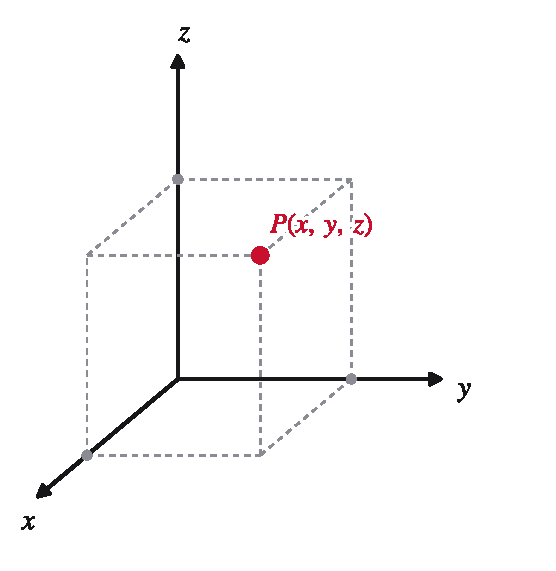
\includegraphics[width=267pt]{fig/m06_f14.pdf}
\caption{Sistema de coordenades cartesianes a l'espai: qualsevol punt $P$ queda determinat per la terna $(x, y, z)$.}
\end{figure}

\section{Components d'un vector a l'espai}

\textbf{Definició:} Els \textbf{components} d'un vector s'obtenen restant ordenadament les coordenades del seu extrem menys les del seu origen. Donats els punts $A(a_1, a_2, a_3)$ i $B(b_1, b_2, b_3)$, el vector $\overrightarrow{AB}$ té components:

\begin{equation}
\overrightarrow{AB} = (b_1 - a_1,\; b_2 - a_2,\; b_3 - a_3)
\end{equation}

Per definir un vector calen tres elements: \textbf{direcció}, \textbf{sentit} i \textbf{magnitud} (mòdul).

Si el vector $\overrightarrow{AB}$ té la mateixa longitud, direcció i sentit que un altre vector $\overrightarrow{CD}$, es tracta de dos vectors \textbf{equipol\textperiodcentered{}lents}. El conjunt de tots els vectors fixos equipol\textperiodcentered{}lents s'anomena \textbf{vector lliure}.

\subsection{Mòdul d'un vector}

El mòdul d'un vector $\vec v = (v_1, v_2, v_3)$ és la seva longitud:

\begin{equation*}
|\vec v| = \sqrt{v_1^2 + v_2^2 + v_3^2}
\end{equation*}

\subsection{Vector unitari}

El vector unitari en la direcció de $\vec v$ és aquell de mòdul 1:

\begin{equation*}
\hat u_v = \frac{\vec v}{|\vec v|}
\end{equation*}

\section{Operacions amb vectors}

\subsection{Suma de vectors}

Donats $\vec a = (a_1, a_2, a_3)$ i $\vec b = (b_1, b_2, b_3)$, el seu vector suma és:

\begin{equation*}
\vec a + \vec b = (a_1 + b_1,\; a_2 + b_2,\; a_3 + b_3)
\end{equation*}

La suma de vectors compleix les propietats següents:

\begin{itemize}
\item \textbf{Commutativa:} $\vec a + \vec b = \vec b + \vec a$
\item \textbf{Associativa:} $\vec a + (\vec b + \vec c) = (\vec a + \vec b) + \vec c$
\item \textbf{Element neutre:} el vector nul $\vec 0 = (0, 0, 0)$ compleix $\vec a + \vec 0 = \vec a$
\item \textbf{Element simètric:} cada vector $\vec a$ té un oposat $-\vec a$ tal que $\vec a + (-\vec a) = \vec 0$
\end{itemize}

\subsection{Multiplicació d'un vector per un escalar}

Donat $k \in \mathbb{R}$ i $\vec a = (a_1, a_2, a_3)$:

\begin{equation*}
k\cdot\vec a = (k a_1,\; k a_2,\; k a_3)
\end{equation*}

Propietats:

\begin{itemize}
\item $k\cdot(\vec a + \vec b) = k\vec a + k\vec b$
\item $1\cdot\vec a = \vec a$
\item $(k + h)\cdot\vec a = k\vec a + h\vec a$
\item $(k\cdot h)\cdot\vec a = k\,(h\cdot\vec a)$
\end{itemize}

\section{Combinació lineal de vectors}

\textbf{Definició:} Donat un conjunt de vectors $\vec v_1, \vec v_2, \vec v_3$ d'un espai vectorial, s'anomena \textbf{combinació lineal} d'aquests vectors tota expressió de la forma

\begin{equation}
\lambda_1\vec v_1 + \lambda_2\vec v_2 + \lambda_3\vec v_3 + \cdots
\end{equation}

on $\lambda_1, \lambda_2, \lambda_3, \ldots \in \mathbb{R}$.

Un vector $\vec v$ és combinació lineal de $\vec v_1, \vec v_2, \vec v_3$ si existeixen $\lambda_1, \lambda_2, \lambda_3$ que verifiquen l'expressió anterior.

\section{Dependència i independència lineal de vectors}

Els vectors $\vec v_1, \vec v_2, \vec v_3$ són \textbf{linealment independents} si l'única solució de

\begin{equation*}
\lambda_1\vec v_1 + \lambda_2\vec v_2 + \lambda_3\vec v_3 = \vec 0
\end{equation*}

és $\lambda_1 = \lambda_2 = \lambda_3 = 0$. En cas contrari, és a dir, si existeix alguna solució amb algun $\lambda_i \neq 0$, els vectors són \textbf{linealment dependents} (un d'ells és combinació lineal dels altres).

\section{Producte escalar de dos vectors}

\textbf{Definició:} El \textbf{producte escalar} de dos vectors $\vec a$ i $\vec b$ és el nombre real

\begin{equation}
\vec a\cdot\vec b = |\vec a|\,|\vec b|\cos\alpha
\end{equation}

on $\alpha$ és l'angle que formen els dos vectors. En components, si $\vec a = (a_1, a_2, a_3)$ i $\vec b = (b_1, b_2, b_3)$:

\begin{equation}
\vec a\cdot\vec b = a_1b_1 + a_2b_2 + a_3b_3
\end{equation}

\subsection{Propietats geomètriques del producte escalar}

La figura següent il\textperiodcentered{}lustra les tres situacions principals:

\begin{figure}[H]
\centering
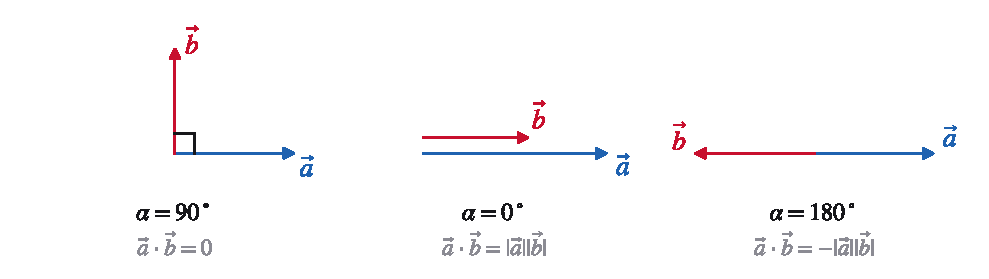
\includegraphics[width=372pt]{fig/m06_f15.pdf}
\caption{Interpretació geomètrica del producte escalar: perpendiculars ($\alpha = 90^\circ$), paral\textperiodcentered{}lels mateix sentit ($\alpha = 0^\circ$) i paral\textperiodcentered{}lels sentit contrari ($\alpha = 180^\circ$).}
\end{figure}

Les propietats geomètriques principals del producte escalar són:

\begin{enumerate}
\item \textbf{Angle entre dos vectors:}
\end{enumerate}

\begin{equation*}
\cos\alpha = \frac{\vec a\cdot\vec b}{|\vec a|\,|\vec b|} \;\Rightarrow\; \alpha = \arccos\!\left(\frac{\vec a\cdot\vec b}{|\vec a|\,|\vec b|}\right)
\end{equation*}

\begin{enumerate}
\item \textbf{Vectors perpendiculars o ortogonals:} $\vec a \perp \vec b$ si i només si $\vec a\cdot\vec b = 0$.
\end{enumerate}

\tema{9}{Equacions de rectes i plans}\section{La recta}

Una recta $r$ queda determinada per qualsevol d'aquestes dades:

\begin{itemize}
\item Dos punts $P$ i $Q$, o equivalentment un punt $P$ i el vector director $\vec u = \overrightarrow{PQ}$.
\item Dos plans $\pi_1$ i $\pi_2$ no paral\textperiodcentered{}lels (la recta és la seva intersecció).
\item Un punt $P$ i un pla $\pi$ perpendicular a la recta.
\end{itemize}

La figura il\textperiodcentered{}lustra els tres casos:

\begin{figure}[H]
\centering
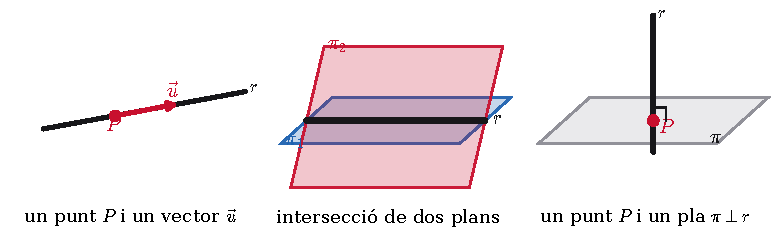
\includegraphics[width=372pt]{fig/m09_f17.pdf}
\caption{Tres maneres de determinar una recta a l'espai.}
\end{figure}

\subsection{Equació vectorial d'una recta}

Donat un punt $P(x_0, y_0, z_0)$ i un vector director $\vec u = (u_1, u_2, u_3)$:

\begin{equation*}
\vec x = \vec p + \lambda\,\vec u, \qquad \forall\lambda\in\mathbb{R}
\end{equation*}

\subsection{Equacions paramètriques d'una recta}

\begin{equation*}
\begin{cases} x = x_0 + \lambda\,u_1 \\ y = y_0 + \lambda\,u_2 \\ z = z_0 + \lambda\,u_3 \end{cases} \qquad \forall\lambda\in\mathbb{R}
\end{equation*}

\subsection{Equacions contínues d'una recta}

Aïllant $\lambda$ de les equacions paramètriques i igualant:

\begin{equation*}
\frac{x - x_0}{u_1} = \frac{y - y_0}{u_2} = \frac{z - z_0}{u_3}
\end{equation*}

\section{El pla}

Un pla $\pi$ queda determinat per qualsevol d'aquestes dades:

\begin{itemize}
\item Tres punts $P$, $Q$ i $R$ no alineats.
\item Un punt $P$ i dos vectors $\vec u$ i $\vec v$ linealment independents (vectors directors del pla).
\item Un punt $P$ i un vector $\vec n \neq \vec 0$ perpendicular al pla (vector normal).
\end{itemize}

\subsection{Equació vectorial d'un pla}

\begin{equation*}
\vec x = \vec p + \lambda\,\vec u + \mu\,\vec v, \qquad \forall\,\lambda,\mu\in\mathbb{R}
\end{equation*}

\subsection{Equacions paramètriques d'un pla}

\begin{equation*}
\begin{cases} x = x_0 + \lambda\,u_1 + \mu\,v_1 \\ y = y_0 + \lambda\,u_2 + \mu\,v_2 \\ z = z_0 + \lambda\,u_3 + \mu\,v_3 \end{cases} \qquad \forall\,\lambda,\mu\in\mathbb{R}
\end{equation*}

\subsection{Equació general (cartesiana) d'un pla}

S'obté desenvolupant el determinant de l'equació vectorial. La forma és:

\begin{equation*}
\begin{vmatrix} x - x_0 & u_1 & v_1 \\ y - y_0 & u_2 & v_2 \\ z - z_0 & u_3 & v_3 \end{vmatrix} = 0 \;\Longrightarrow\; Ax + By + Cz + D = 0
\end{equation*}

\section{Vector associat a un pla}

Donat el pla $\pi: Ax + By + Cz + D = 0$, el vector $\vec n = (A, B, C)$ és perpendicular al pla i s'anomena \textbf{vector normal} o \textbf{vector associat}.

\begin{figure}[H]
\centering
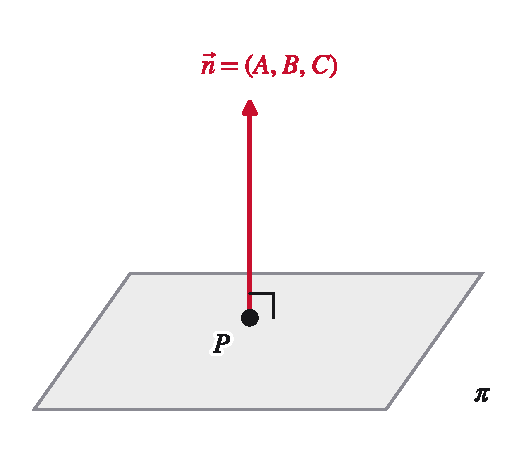
\includegraphics[width=248pt]{fig/m09_f18.pdf}
\caption{El vector normal $\vec n = (A, B, C)$ és perpendicular al pla $Ax + By + Cz + D = 0$.}
\end{figure}

\section{Recta determinada per dos plans}

La intersecció de dos plans no paral\textperiodcentered{}lels determina una recta:

\begin{equation*}
r: \begin{cases} Ax + By + Cz + D = 0 \\ A'x + B'y + C'z + D' = 0 \end{cases}
\end{equation*}

Perquè els dos plans determinin una recta cal que siguin no paral\textperiodcentered{}lels, és a dir, que els seus vectors normals $\vec n_1 = (A, B, C)$ i $\vec n_2 = (A', B', C')$ no siguin proporcionals. El vector director de la recta resultant és $\vec u = \vec n_1 \times \vec n_2$.

\section{Feix de plans}

\textbf{Definició:} El \textbf{feix de plans} és el conjunt de tots els plans que contenen (o passen per) una mateixa recta $r$. El vector normal de cadascun dels plans del feix és perpendicular a $r$.

Si la recta $r$ és la intersecció dels plans $\pi_1: A_1x + B_1y + C_1z + D_1 = 0$ i $\pi_2: A_2x + B_2y + C_2z + D_2 = 0$, qualsevol pla del feix es pot expressar com:

\begin{equation*}
\lambda\,(A_1x + B_1y + C_1z + D_1) + \mu\,(A_2x + B_2y + C_2z + D_2) = 0, \qquad (\lambda, \mu) \neq (0, 0)
\end{equation*}

\section{Complement: mètode per obtenir equacions}

\subsection{Recta per dos punts}

Per a la recta que passa per $A$ i $B$: es pren $A$ com a punt i $\vec d=\overrightarrow{AB}$ com a vector director.

\emph{Exemple:} Recta per $A(1,2,3)$ i $B(3,0,4)$. Vector director $\vec d=(2,-2,1)$.

\begin{equation*}
\begin{cases}x=1+2t\\y=2-2t\\z=3+t\end{cases}\qquad\Longleftrightarrow\qquad\frac{x-1}{2}=\frac{y-2}{-2}=\frac{z-3}{1}
\end{equation*}

\subsection{Pla per tres punts}

Es prenen dos vectors del pla, $\overrightarrow{AB}$ i $\overrightarrow{AC}$; el vector normal és el seu producte vectorial, i amb ell s'escriu $Ax+By+Cz+D=0$ imposant que passi per $A$.

\emph{Exemple:} Pla per $A(1,0,0)$, $B(0,1,0)$ i $C(0,0,1)$. $\overrightarrow{AB}=(-1,1,0)$ i $\overrightarrow{AC}=(-1,0,1)$, i

\begin{equation*}
\vec n=\overrightarrow{AB}\times\overrightarrow{AC}=(1,1,1)\;\Rightarrow\;x+y+z+D=0,\ \ A\in\pi\Rightarrow D=-1
\end{equation*}

El pla és $\pi:\ x+y+z-1=0$.

\emph{Alternativa:} $\begin{vmatrix}x-1&y&z\\-1&1&0\\-1&0&1\end{vmatrix}=0$ dóna el mateix pla.

\subsection{Passar d'una forma a una altra}

\textbf{De contínua a implícita} (dos plans). Se separen les igualtats de dues en dues.

\emph{Exemple:} $\dfrac{x-1}{2}=\dfrac{y+1}{-1}=\dfrac{z}{3}$.

\begin{itemize}
\item Primera i segona: $-(x-1)=2(y+1)\Rightarrow x+2y+1=0$.
\item Segona i tercera: $3(y+1)=-z\Rightarrow 3y+z+3=0$.
\end{itemize}

\begin{equation*}
r:\ \begin{cases}x+2y+1=0\\3y+z+3=0\end{cases}
\end{equation*}

\textbf{De implícita a paramètrica.} Es resol el sistema prenent una incògnita com a paràmetre.

\emph{Exemple:} $\begin{cases}x+y-z=1\\2x-y+z=2\end{cases}$. Sumant: $3x=3\Rightarrow x=1$. Llavors $y-z=0$; prenem $z=t$ i $y=t$.

\begin{equation*}
r:\ (x,y,z)=(1,0,0)+t\,(0,1,1)
\end{equation*}

\emph{Un cop tens un punt i un vector director, tens tot el que cal per al tema 10 i 11.}

\tema{10}{Posició relativa de rectes i plans}\section{Posició relativa de dos plans}

Donats dos plans $\pi: Ax + By + Cz + D = 0$ i $\pi': A'x + B'y + C'z + D' = 0$, la posició relativa es determina comparant els coeficients:

\begin{table}[H]
\centering
\renewcommand{\arraystretch}{1.25}
\begin{tabularx}{\textwidth}{lc>{\raggedright\arraybackslash}X}
\toprule
Plans coincidents & Plans paral\textperiodcentered{}lels & Plans secants \\
\midrule
$\dfrac{A}{A'} = \dfrac{B}{B'} = \dfrac{C}{C'} = \dfrac{D}{D'}$ & $\dfrac{A}{A'} = \dfrac{B}{B'} = \dfrac{C}{C'} \neq \dfrac{D}{D'}$ & No hi ha proporcionalitat entre els coeficients. La intersecció és una recta $r$. \\
\bottomrule
\end{tabularx}
\end{table}

\begin{figure}[H]
\centering
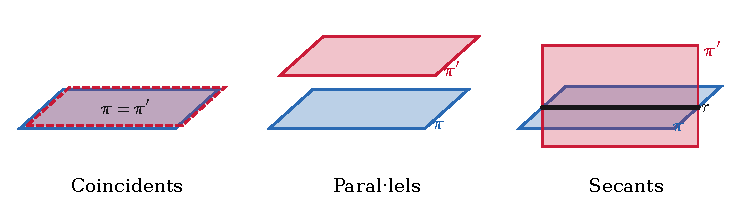
\includegraphics[width=372pt]{fig/m10_f19.pdf}
\caption{Posició relativa de dos plans: coincidents, paral\textperiodcentered{}lels i secants.}
\end{figure}

\section{Posició relativa de tres plans}

Amb tres plans, s'aplica el \textbf{Teorema de Rouché-Frobenius} sobre la matriu de coeficients $M$ i la matriu ampliada $M'$:

\begin{table}[H]
\centering
\renewcommand{\arraystretch}{1.25}
\begin{tabularx}{\textwidth}{lc>{\raggedright\arraybackslash}Xc}
\toprule
$\operatorname{Rg}(M)$ & $\operatorname{Rg}(M')$ & Posició relativa & Tipus \\
\midrule
1 & 1 & Tres plans coincidents & S.C.I \\
1 & 2 & Tres plans paral\textperiodcentered{}lels & S.I \\
2 & 2 & Tres plans secants a una recta $r$ comú & S.C.I \\
2 & 2 & Dos plans coincidents, l'altre secant als dos & S.C.I \\
2 & 3 & Prisma: plans secants dos a dos & S.I \\
2 & 3 & Dos plans paral\textperiodcentered{}lels, l'altre secant als dos & S.I \\
3 & 3 & Triedre: tres plans secants a un punt & S.C.D \\
\bottomrule
\end{tabularx}
\end{table}

\section{Posició relativa de recta i pla}

Per estudiar la posició de la recta $r$ i el pla $\pi$, es substitueixen les equacions paramètriques de $r$ a l'equació de $\pi$ i s'analitza el sistema resultant:

\begin{table}[H]
\centering
\renewcommand{\arraystretch}{1.25}
\begin{tabularx}{\textwidth}{>{\raggedright\arraybackslash}X>{\raggedright\arraybackslash}X>{\raggedright\arraybackslash}X}
\toprule
S.C.D & S.C.I & S.I \\
\midrule
$r$ i $\pi$ tenen un punt en comú (recta \textbf{secant} al pla) & $r$ està \textbf{continguda} en $\pi$ & $r$ i $\pi$ no tenen cap punt en comú (recta \textbf{paral\textperiodcentered{}lela} al pla) \\
\bottomrule
\end{tabularx}
\end{table}

\begin{figure}[H]
\centering
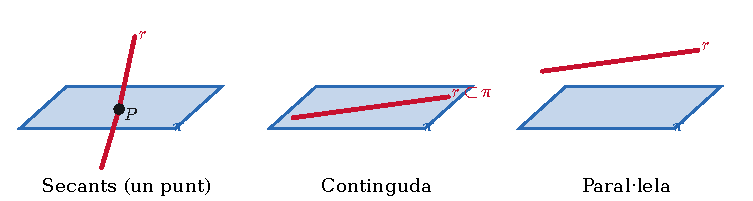
\includegraphics[width=372pt]{fig/m10_f20.pdf}
\caption{Les tres posicions relatives d'una recta i un pla.}
\end{figure}

\section{Posició relativa de dues rectes}

Expressades $r$ i $s$ com a intersecció de dos plans cadascuna, es forma un sistema de quatre equacions. Aplicant el TRF sobre la matriu $M$ i l'ampliada $M'$:

\begin{table}[H]
\centering
\renewcommand{\arraystretch}{1.25}
\begin{tabular}{lccc}
\toprule
S.C.D & S.C.I & S.I (1) & S.I (2) \\
\midrule
$\operatorname{Rg}(M) = 3 = \operatorname{Rg}(M')$ & $\operatorname{Rg}(M) = 2 = \operatorname{Rg}(M')$ & $\operatorname{Rg}(M) = 2 \neq \operatorname{Rg}(M') = 3$ & $\operatorname{Rg}(M) = 3 \neq \operatorname{Rg}(M') = 4$ \\
Rectes \textbf{secants} & Rectes \textbf{coincidents} & Rectes \textbf{paral\textperiodcentered{}leles} & Rectes que \textbf{s'encreuen} \\
\bottomrule
\end{tabular}
\end{table}

\subsection{Resum per vectors directors}

Donats els vectors directors $\vec u$ i $\vec v$ de $r$ i $s$, i el vector $\overrightarrow{PQ}$ entre un punt de cada recta:

\begin{itemize}
\item Si $\vec u = \lambda\vec v$ (vectors proporcionals, rectes paral\textperiodcentered{}leles o coincidents):
\begin{itemize}
\item $\overrightarrow{PQ} = \mu\,\vec u \Rightarrow$ rectes \textbf{coincidents}
\item $\overrightarrow{PQ} \neq \mu\,\vec u \Rightarrow$ rectes \textbf{paral\textperiodcentered{}leles}
\end{itemize}
\item Si $\vec u \neq \lambda\vec v$ (vectors no proporcionals):
\begin{itemize}
\item $D(\vec u, \vec v, \overrightarrow{PQ}) = 0 \Rightarrow$ rectes \textbf{secants}
\item $D(\vec u, \vec v, \overrightarrow{PQ}) \neq 0 \Rightarrow$ rectes que \textbf{s'encreuen}
\end{itemize}
\end{itemize}

on $D(\vec u, \vec v, \overrightarrow{PQ})$ és el determinant format per les tres files $\vec u$, $\vec v$ i $\overrightarrow{PQ}$.

\section{Perpendicularitat}

\subsection{Plans perpendiculars}

Dos plans $\pi_1$ i $\pi_2$ amb vectors normals $\vec n = (A, B, C)$ i $\vec n' = (A', B', C')$ són perpendiculars si:

\begin{equation*}
\vec n\cdot\vec n' = 0 \;\Longrightarrow\; AA' + BB' + CC' = 0
\end{equation*}

\subsection{Recta i pla perpendiculars}

Una recta de vector director $\vec v = (V_1, V_2, V_3)$ és perpendicular al pla $Ax + By + Cz + D = 0$ si $\vec v$ és proporcional al vector normal $\vec n = (A, B, C)$:

\begin{equation*}
\vec v = k\,\vec n,\; k \neq 0 \iff \frac{V_1}{A} = \frac{V_2}{B} = \frac{V_3}{C}
\end{equation*}

\subsection{Rectes perpendiculars}

Dues rectes amb vectors directors $\vec v$ i $\vec u$ són perpendiculars si:

\begin{equation*}
\vec v\cdot\vec u = 0
\end{equation*}

\section{Projeccions ortogonals sobre un pla}

\subsection{Projecció ortogonal d'un punt sobre un pla}

El punt $P'$ és la \textbf{projecció ortogonal} de $P$ sobre el pla $\pi$ si $P'$ és el peu de la perpendicular a $\pi$ que passa per $P$. Es troba com la intersecció de $\pi$ amb la recta perpendicular a $\pi$ que passa per $P$.

\begin{figure}[H]
\centering
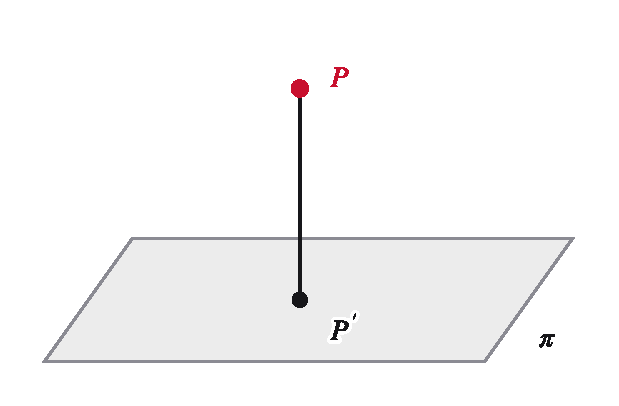
\includegraphics[width=297pt]{fig/m10_f21.pdf}
\caption{Projecció ortogonal del punt $P$ sobre el pla $\pi$: el punt $P'$ és el peu de la perpendicular.}
\end{figure}

\subsection{Projecció ortogonal d'una recta sobre un pla}

La projecció ortogonal d'una recta $r$ sobre un pla $\pi$ és la recta $r'$ que resulta d'intersectar $\pi$ amb el pla que conté $r$ i és perpendicular a $\pi$. Per a un segment $PQ$, es projecten els extrems $P$ i $Q$ per obtenir $P'$ i $Q'$.

\subsection{Projecció ortogonal d'un punt sobre una recta}

La projecció ortogonal del punt $P$ sobre la recta $r$ és el punt $P'$ intersecció de $r$ amb el pla perpendicular a $r$ que passa per $P$. El vector normal d'aquest pla coincideix amb el vector director de $r$.

\tema{11}{Distàncies i angles}\section{Distància entre dos punts}

Donats $P = (x_1, y_1, z_1)$ i $Q = (x_2, y_2, z_2)$, la distància és el mòdul del vector $\overrightarrow{PQ}$:

\begin{equation*}
d(P, Q) = |\overrightarrow{PQ}| = \sqrt{(x_2 - x_1)^2 + (y_2 - y_1)^2 + (z_2 - z_1)^2}
\end{equation*}

\section{Distància d'un punt a una recta}

La distància entre el punt $P$ i la recta $r$ és $d(P, r) = d(P, P')$, on $P'$ és la projecció ortogonal de $P$ sobre $r$. Es pot calcular de dues maneres:

\begin{enumerate}
\item \textbf{Mètode geomètric:} trobar $P'$ (intersecció del pla $\perp r$ per $P$ amb $r$) i calcular $d(P, P')$.
\item \textbf{Mitjançant el producte vectorial} (si $\vec u$ és el vector director de $r$ i $Q \in r$):
\end{enumerate}

\begin{equation*}
d(P, r) = \frac{|\vec u\times\overrightarrow{QP}|}{|\vec u|}
\end{equation*}

\begin{figure}[!htbp]
\centering
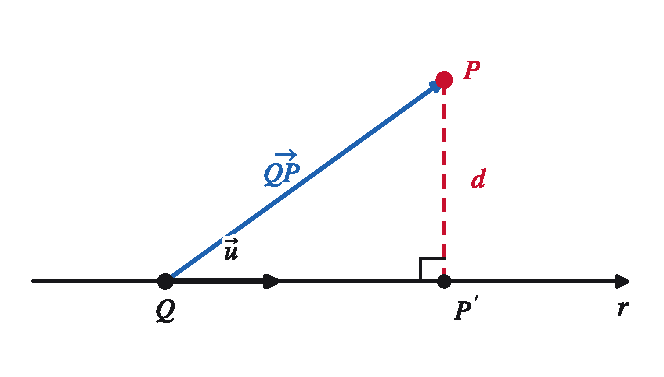
\includegraphics[width=319pt]{fig/m11_f22.pdf}
\caption{Distància del punt $P$ a la recta $r$: $d = |\vec u\times\overrightarrow{QP}|\,/\,|\vec u|$.}
\end{figure}

\section{Distància d'un punt a un pla}

La distància del punt $P(x_0, y_0, z_0)$ al pla $\pi: Ax + By + Cz + D = 0$ és $d(P, \pi) = d(P, P')$, on $P'$ és el peu de la perpendicular. La fórmula directa és:

\begin{equation*}
d(P, \pi) = \frac{|Ax_0 + By_0 + Cz_0 + D|}{\sqrt{A^2 + B^2 + C^2}}
\end{equation*}

\begin{figure}[!htbp]
\centering
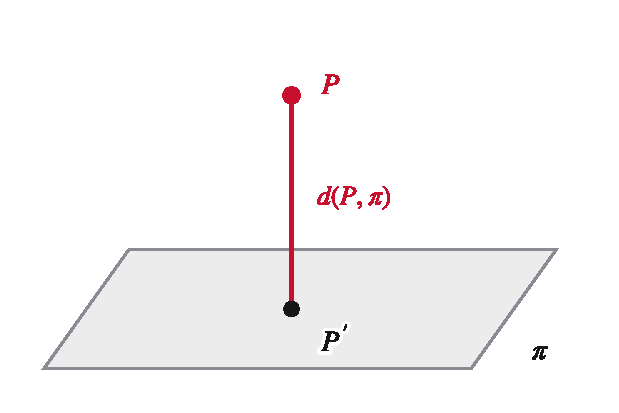
\includegraphics[width=297pt]{fig/m11_f23.pdf}
\caption{Distància del punt $P$ al pla $\pi$: la longitud del segment perpendicular a $\pi$ que passa per $P$.}
\end{figure}

\section{Distàncies entre rectes i plans}

\subsection{Distància entre dues rectes}

\begin{itemize}
\item \textbf{Secants o coincidents:} $d = 0$.
\item \textbf{Paral\textperiodcentered{}leles:} $d(r, s) = d(P, s)$, on $P$ és qualsevol punt de $r$.
\item \textbf{Que s'encreuen:} existeix una única recta $t$ perpendicular a ambdues. Si $P \in r$ i $P' \in s$ són els punts de contacte de $t$, aleshores $d(r, s) = d(P, P')$. Fórmula amb el producte mixt (apartat 8):
\end{itemize}

\begin{equation*}
d(r, s) = \frac{|[\overrightarrow{PQ}, \vec u, \vec v]|}{|\vec u\times\vec v|}
\end{equation*}

on $P \in r$, $Q \in s$, $\vec u$ i $\vec v$ són els vectors directors de $r$ i $s$.

\subsection{Distància entre una recta i un pla}

\begin{itemize}
\item Si la recta talla el pla o hi és continguda: $d = 0$.
\item Si la recta és paral\textperiodcentered{}lela al pla: $d(r, \pi) = d(P, \pi)$, on $P$ és qualsevol punt de $r$.
\end{itemize}

\subsection{Distància entre dos plans}

\begin{itemize}
\item Si es tallen o són coincidents: $d = 0$.
\item Si són paral\textperiodcentered{}lels: $d(\pi_1, \pi_2) = d(P, \pi_2)$, on $P$ és qualsevol punt de $\pi_1$.
\end{itemize}

\section{Angles formats per rectes i plans}

L'angle entre dos vectors $\vec v$ i $\vec w$ és:

\begin{equation*}
\vec v\cdot\vec w = |\vec v|\,|\vec w|\cos\alpha \;\Longrightarrow\; \alpha = \arccos\frac{\vec v\cdot\vec w}{|\vec v|\,|\vec w|}
\end{equation*}

\subsection{Angle entre dues rectes}

L'angle format per $r$ i $s$ és el més petit dels angles formats pels seus vectors directors $\vec u$ i $\vec v$ (es pren valor absolut per garantir un angle agut):

\begin{equation*}
\cos\alpha = \frac{|\vec u\cdot\vec v|}{|\vec u|\,|\vec v|} \;\Rightarrow\; \alpha = \arccos\frac{|\vec u\cdot\vec v|}{|\vec u|\,|\vec v|}
\end{equation*}

\subsection{Angle entre una recta i un pla}

L'angle $\alpha$ entre la recta $r$ (vector director $\vec u$) i el pla $\pi$ (vector normal $\vec n$) és el complement de l'angle $\beta$ entre $\vec u$ i $\vec n$:

\begin{equation*}
\sin\alpha = \cos\beta = \frac{|\vec u\cdot\vec n|}{|\vec u|\,|\vec n|} \;\Rightarrow\; \alpha = \arcsin\frac{|\vec u\cdot\vec n|}{|\vec u|\,|\vec n|}
\end{equation*}

\begin{figure}[!htbp]
\centering
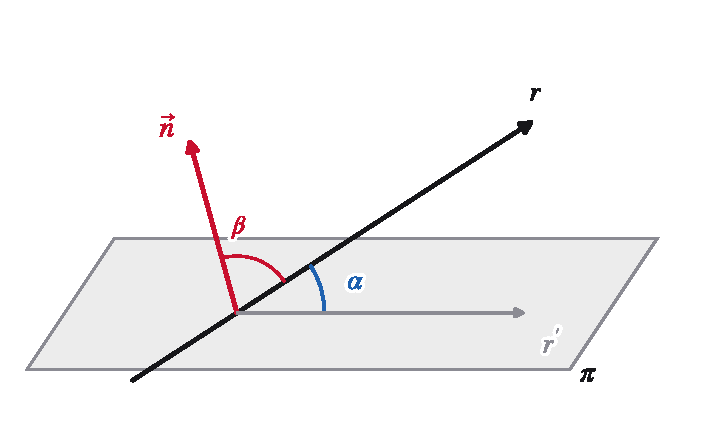
\includegraphics[width=341pt]{fig/m11_f24.pdf}
\caption{Angle $\alpha$ entre la recta $r$ i el pla $\pi$: $\sin\alpha = \cos\beta = |\vec u\cdot\vec n|\,/\,(|\vec u||\vec n|)$.}
\end{figure}

\subsection{Angle entre dos plans}

L'angle entre $\pi_1$ i $\pi_2$ (amb vectors normals $\vec n_1$ i $\vec n_2$) és el més petit dels angles diedres:

\begin{equation*}
\cos\alpha = \frac{|\vec n_1\cdot\vec n_2|}{|\vec n_1|\,|\vec n_2|} \;\Rightarrow\; \alpha = \arccos\frac{|\vec n_1\cdot\vec n_2|}{|\vec n_1|\,|\vec n_2|}
\end{equation*}

\section{Producte vectorial de dos vectors}

\textbf{Definició:} El \textbf{producte vectorial} de $\vec u = (u_1, u_2, u_3)$ i $\vec v = (v_1, v_2, v_3)$ és el vector

\begin{equation}
\vec u\times\vec v = \begin{vmatrix} \vec e_1 & u_1 & v_1 \\ \vec e_2 & u_2 & v_2 \\ \vec e_3 & u_3 & v_3 \end{vmatrix} = (u_2v_3 - u_3v_2,\; u_3v_1 - u_1v_3,\; u_1v_2 - u_2v_1)
\end{equation}

Les característiques del vector $\vec u\times\vec v$ són:

\begin{itemize}
\item \textbf{Mòdul:} $|\vec u\times\vec v| = |\vec u|\,|\vec v|\sin\alpha$, amb $0^\circ \le \alpha \le 180^\circ$.
\item \textbf{Direcció:} perpendicular als dos vectors $\vec u$ i $\vec v$.
\item \textbf{Sentit:} el d'avanç d'un tirabuixó que giri de $\vec u$ a $\vec v$ en el menor angle possible (regla de la mà dreta).
\end{itemize}

\emph{Observació:} si $\vec u\cdot\vec v = 0$, els vectors són perpendiculars i $|\vec u\times\vec v| = |\vec u|\,|\vec v|$ (valor màxim).

\section{Aplicacions geomètriques del producte vectorial}

\subsection{Àrea d'un paral\textperiodcentered{}lelogram}

Si $\vec u$ i $\vec v$ són dos costats adjacents del paral\textperiodcentered{}lelogram:

\begin{equation*}
A = |\vec u\times\vec v|
\end{equation*}

\subsection{Àrea d'un triangle}

Donats tres vèrtexs $P$, $Q$, $R$:

\begin{equation*}
A = \frac12\,|\overrightarrow{PQ}\times\overrightarrow{PR}|
\end{equation*}

\subsection{Distància d'un punt a una recta (forma alternativa)}

Si $Q \in r$ i $\vec u$ és el vector director de $r$:

\begin{equation*}
d(P, r) = \frac{|\vec u\times\overrightarrow{QP}|}{|\vec u|}
\end{equation*}

\section{Producte mixt de tres vectors}

\textbf{Definició:} El \textbf{producte mixt} dels vectors $\vec u$, $\vec v$ i $\vec w$ és el nombre real

\begin{equation}
[\vec u, \vec v, \vec w] = \vec u\cdot(\vec v\times\vec w) = \begin{vmatrix} u_1 & u_2 & u_3 \\ v_1 & v_2 & v_3 \\ w_1 & w_2 & w_3 \end{vmatrix}
\end{equation}

\section{Aplicacions geomètriques del producte mixt}

\subsection{Volum d'un paral\textperiodcentered{}lelepípede}

Si $\vec u$, $\vec v$ i $\vec w$ són tres arestes adjacents:

\begin{equation*}
V = |[\vec u, \vec v, \vec w]|
\end{equation*}

\subsection{Volum d'una piràmide de base triangular}

\begin{equation*}
V = \frac16\,|[\vec u, \vec v, \vec w]|
\end{equation*}

\subsection{Distància entre dues rectes que s'encreuen}

Si $P \in r$, $Q \in s$, i $\vec u$, $\vec v$ són els vectors directors de $r$ i $s$:

\begin{equation*}
|[\overrightarrow{PQ}, \vec u, \vec v]| = |\vec u\times\vec v|\cdot d(r, s) \;\Longrightarrow\; d(r, s) = \frac{|[\overrightarrow{PQ}, \vec u, \vec v]|}{|\vec u\times\vec v|}
\end{equation*}

\section{Complement: punts i figures simètriques}

\subsection{Mètode general}

El \textbf{simètric} $P'$ d'un punt $P$ respecte d'un element (punt, recta o pla) es troba trobant primer el \textbf{punt mitjà} $M$ entre $P$ i $P'$ i després aïllant:

\begin{equation*}
M=\frac{P+P'}{2}\quad\Longrightarrow\quad P'=2M-P
\end{equation*}

\begin{table}[!htbp]
\centering
\renewcommand{\arraystretch}{1.3}
\begin{tabularx}{\textwidth}{l>{\raggedright\arraybackslash}X}
\toprule
Respecte de\ldots{} & Com trobar $M$ \\
\midrule
un punt $Q$ & $M=Q$ \\
una recta $r$ & $M=r\cap\pi$, on $\pi$ és el pla per $P$ \textbf{perpendicular} a $r$ (vector normal $=\vec d_r$) \\
un pla $\pi$ & $M=r\cap\pi$, on $r$ és la recta per $P$ \textbf{perpendicular} a $\pi$ (vector director $=\vec n_\pi$) \\
\bottomrule
\end{tabularx}
\end{table}

\begin{figure}[!htbp]
\centering
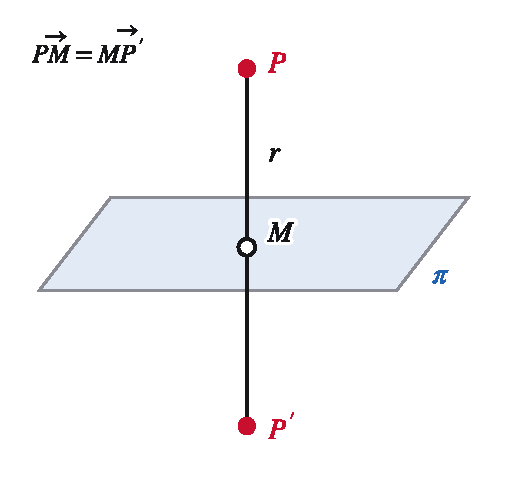
\includegraphics[width=251pt]{fig/m11_f37.pdf}
\caption{El simètric $P'$ de $P$ respecte d'un pla: $M$ és la intersecció de la perpendicular $r$ amb el pla i és el punt mitjà de $PP'$.}
\end{figure}

\subsection{Exemple 1 --- Simètric respecte d'un pla}

Simètric de $P(1,2,3)$ respecte de $\pi:\ x+y+z-3=0$.

\begin{enumerate}
\item Recta perpendicular per $P$: $r:\ (1+t,\,2+t,\,3+t)$.
\item Intersecció amb $\pi$: $(1+t)+(2+t)+(3+t)-3=0\Rightarrow 3+3t=0\Rightarrow t=-1$, de manera que $M=(0,1,2)$.
\item $P'=2M-P=(2\cdot0-1,\,2\cdot1-2,\,2\cdot2-3)=(-1,0,1)$.
\end{enumerate}

\emph{Comprovació:} $-1+0+1-3=-3$ i $1+2+3-3=3$: estan a banda i banda del pla i a la mateixa distància $\checkmark$.

\subsection{Exemple 2 --- Simètric respecte d'una recta}

Simètric de $P(1,2,0)$ respecte de $r:\ (t,\,t,\,0)$ amb $\vec d=(1,1,0)$.

\begin{enumerate}
\item Pla per $P$ perpendicular a $r$: $x+y+D=0$ i $1+2+D=0\Rightarrow D=-3$, així que $\pi:\ x+y-3=0$.
\item $M=r\cap\pi$: $t+t-3=0\Rightarrow t=\frac32$ i $M=\left(\frac32,\frac32,0\right)$.
\item $P'=2M-P=(3-1,\,3-2,\,0)=(2,1,0)$.
\end{enumerate}

\subsection{Pla mediador}

El \textbf{pla mediador} d'un segment $AB$ és el pla perpendicular a $AB$ pel seu punt mitjà: conté tots els punts equidistants d'$A$ i $B$.

\emph{Exemple:} $A(1,0,2)$ i $B(3,2,0)$. $\overrightarrow{AB}=(2,2,-2)\parallel(1,1,-1)$ i $M=(2,1,1)$. Llavors $x+y-z+D=0$ amb $2+1-1+D=0\Rightarrow D=-2$:

\begin{equation*}
\pi:\ x+y-z-2=0
\end{equation*}

\section{Complement: interpretació geomètrica dels productes vectorial i mixt}

\begin{figure}[!htbp]
\centering
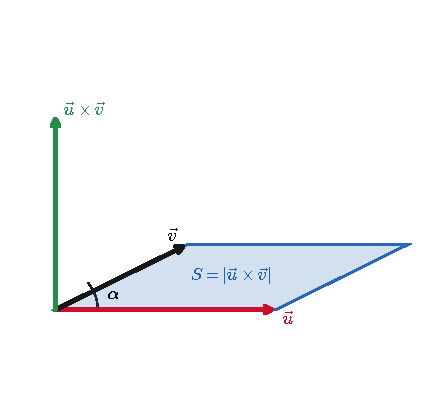
\includegraphics[width=208pt]{fig/x11_cross.pdf}
\caption{El producte vectorial $\vec u\times\vec v$ és perpendicular al pla que formen $\vec u$ i $\vec v$ (regla de la mà dreta) i el seu mòdul és l'àrea del paral\textperiodcentered{}lelogram.}
\end{figure}

El sentit de $\vec u\times\vec v$ es determina amb la \textbf{regla de la mà dreta}: si els dits van de $\vec u$ cap a $\vec v$ pel camí més curt, el polze indica el sentit del producte. Per això $\vec v\times\vec u=-\,\vec u\times\vec v$.

\begin{figure}[!htbp]
\centering
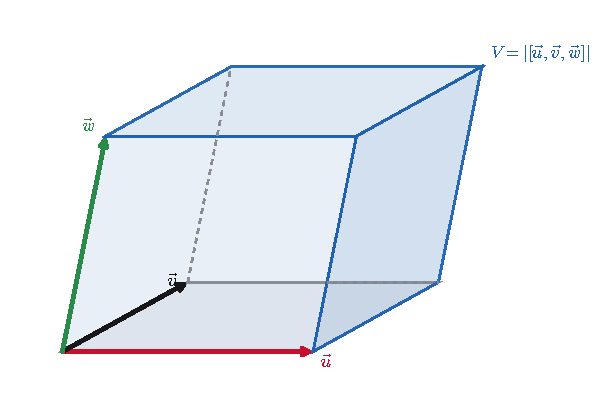
\includegraphics[width=286pt]{fig/x11_parallelepiped.pdf}
\caption{El valor absolut del producte mixt $[\vec u,\vec v,\vec w]$ és el volum del paral\textperiodcentered{}lelepípede definit pels tres vectors.}
\end{figure}

El producte mixt es calcula com a determinant: $[\vec u,\vec v,\vec w]=\begin{vmatrix}u_1&u_2&u_3\\v_1&v_2&v_3\\w_1&w_2&w_3\end{vmatrix}$. Si val $0$, els tres vectors són coplanaris.

\section{Complement: exemples resolts de distàncies, angles i volums}

\emph{Exemple 1 --- Distància d'un punt a un pla:} $P(1,2,3)$ i $\pi:\ 2x-y+2z-4=0$:

\begin{equation*}
d(P,\pi)=\frac{|2\cdot1-2+2\cdot3-4|}{\sqrt{2^2+(-1)^2+2^2}}=\frac{2}{3}.
\end{equation*}

\emph{Exemple 2 --- Distància entre dues rectes que s'encreuen:} $r:(0,0,0)+t(1,0,0)$ i $s:(0,1,0)+u(0,0,1)$. $\vec u\times\vec v=(0,-1,0)$, $\overrightarrow{PQ}=(0,1,0)$ i $[\vec u,\vec v,\overrightarrow{PQ}]=-1$:

\begin{equation*}
d(r,s)=\frac{|[\vec u,\vec v,\overrightarrow{PQ}]|}{|\vec u\times\vec v|}=\frac11=1.
\end{equation*}

\emph{Exemple 3 --- Angle entre dos plans:} $\pi:x+y+z=0$ i $\pi':x+y=0$, amb $\vec n=(1,1,1)$ i $\vec n'=(1,1,0)$:

\begin{equation*}
\cos\alpha=\frac{|\vec n\cdot\vec n'|}{|\vec n|\,|\vec n'|}=\frac{2}{\sqrt3\,\sqrt2}=\frac{2}{\sqrt6}\ \Rightarrow\ \alpha\approx35{,}3^{\circ}.
\end{equation*}

\emph{Exemple 4 --- Angle entre una recta i un pla:} $r$ de vector director $\vec u=(1,2,2)$ i el pla $z=0$ ($\vec n=(0,0,1)$): $\sin\alpha=\dfrac{|\vec u\cdot\vec n|}{|\vec u|\,|\vec n|}=\dfrac23\Rightarrow\alpha\approx41{,}8^{\circ}$.

\emph{Exemple 5 --- Àrea d'un triangle i volum d'un tetraedre:} Siguin $A(1,0,0)$, $B(0,2,0)$, $C(0,0,3)$ i $O(0,0,0)$.

\begin{itemize}
\item $\overrightarrow{AB}=(-1,2,0)$ i $\overrightarrow{AC}=(-1,0,3)$; $\overrightarrow{AB}\times\overrightarrow{AC}=(6,3,2)$ amb mòdul $7$. Àrea del triangle $ABC=\dfrac72$.
\item El volum del tetraedre $OABC$ és $\dfrac16\bigl|[\overrightarrow{OA},\overrightarrow{OB},\overrightarrow{OC}]\bigr|=\dfrac16\cdot6=1$.
\item El pla $ABC$ és $\dfrac x1+\dfrac y2+\dfrac z3=1$, és a dir, $6x+3y+2z-6=0$, i la distància d'$O$ a aquest pla és $\dfrac{6}{7}$. Comprovació: $V=\dfrac13\cdot\dfrac72\cdot\dfrac67=1$.
\end{itemize}

\emph{Exemple 6 --- Distància d'un punt a una recta:} $P(1,1,1)$ i $r:(0,0,0)+t(1,0,0)$. $\overrightarrow{QP}=(1,1,1)$ i $\vec u\times\overrightarrow{QP}=(0,-1,1)$, de mòdul $\sqrt2$: $d(P,r)=\dfrac{\sqrt2}{1}=\sqrt2$.

% ---------------------------------------------------------------- Bloc 4
\blocitems{\begin{itemize}\item Tema 12. Probabilitat\end{itemize}}
\bloc{4}{Probabilitat}{Probabilitat condicionada, variables aleatòries, distribució binomial i distribució normal.}
\tema{12}{Probabilitat}\section{Probabilitat condicionada}

\textbf{Definició:} Siguin $A$ i $B$ dos successos d'un espai mostral $S$, amb $p(A) \neq 0$. S'anomena \textbf{probabilitat de $B$ condicionada a $A$} el quocient

\begin{equation}
p(B/A) = \frac{p(A\cap B)}{p(A)}
\end{equation}

Es llegeix: ``probabilitat del succés $B$ sabent que s'ha verificat el succés $A$''.

D'aquesta definició s'obtenen les \textbf{regles del producte}:

\begin{equation*}
p(A\cap B) = p(A)\cdot p(B/A) = p(B)\cdot p(A/B)
\end{equation*}

\textbf{Definició:} El succés $B$ és \textbf{independent} del succés $A$ si $p(B/A) = p(B)$. La relació és simètrica: si $B$ és independent de $A$, llavors $A$ és independent de $B$. En aquest cas:

\begin{equation}
p(A\cap B) = p(A)\cdot p(B)
\end{equation}

Si en canvi $p(A\cap B) \neq p(A)\cdot p(B)$, els successos són \textbf{dependents} i cal usar les fórmules de la probabilitat condicionada.

\section{Fórmula de Bayes}

Siguin $A_1, A_2, \ldots, A_k$ successos incompatibles dos a dos ($A_i\cap A_j = \varnothing$ per $i \neq j$) i exhaustius ($A_1\cup A_2\cup\cdots\cup A_k = \Omega$). Per a qualsevol succés $B$, el \textbf{teorema de la probabilitat total} dona:

\begin{equation*}
p(B) = p(A_1)\cdot p(B/A_1) + p(A_2)\cdot p(B/A_2) + \cdots + p(A_k)\cdot p(B/A_k)
\end{equation*}

La \textbf{fórmula de Bayes} permet calcular la probabilitat a posteriori de cada $A_j$ sabent que ha ocorregut $B$:

\begin{equation*}
p(A_j/B) = \frac{p(A_j)\cdot p(B/A_j)}{p(A_1)\cdot p(B/A_1) + p(A_2)\cdot p(B/A_2) + \cdots + p(A_k)\cdot p(B/A_k)}
\end{equation*}

\section{Variable aleatòria i funció de probabilitat}

\textbf{Definició:} Donat un espai mostral $\Omega$, una \textbf{variable aleatòria} $X$ és una aplicació

\begin{equation}
X: \Omega \to \mathbb{R}
\end{equation}

que assigna un nombre real a cada resultat possible de l'experiment.

Una variable aleatòria és \textbf{discreta} si el conjunt de valors que pot prendre és finit o numerable: $\{x_1, x_2, \ldots, x_n\}$.

\textbf{Definició:} La \textbf{funció de probabilitat} (o llei de probabilitat) d'una variable aleatòria discreta $X$ assigna a cada valor $x_i$ la seva probabilitat:

\begin{equation}
p[X = x_i] = p_i, \qquad \forall\, i = 1, 2, \ldots, n
\end{equation}

Ha de complir: $p_i \ge 0$ i $\displaystyle\sum_{i=1}^{n} p_i = 1$.

\section{Distribució binomial}

\textbf{Definició:} Una variable aleatòria $X$ segueix una \textbf{distribució binomial} $B(n, p)$ quan es realitza un experiment de Bernoulli (resultat èxit o fracàs, amb probabilitat d'èxit $p$) un total de $n$ proves independents. La funció de probabilitat és:

\begin{equation}
p[X = k] = \binom{n}{k}p^k(1-p)^{n-k} = \binom{n}{k}p^kq^{n-k}, \qquad k = 0, 1, \ldots, n
\end{equation}

on $q = 1 - p$.

Les condicions per aplicar la distribució binomial $B(n, p)$ són:

\begin{itemize}
\item El resultat de cada prova pertany a una de dues categories: èxit o fracàs.
\item La probabilitat d'èxit $p$ és constant en cada prova.
\item Les $n$ proves són independents entre si.
\end{itemize}

Les característiques principals de $B(n, p)$ són:

\begin{itemize}
\item \textbf{Esperança (mitjana):} $\mu = E[X] = np$
\item \textbf{Variància:} $\sigma^2 = npq = np(1-p)$
\item \textbf{Desviació típica:} $\sigma = \sqrt{npq}$
\end{itemize}

\section{Complement: distribució normal}

\subsection{Variable aleatòria contínua}

Una variable aleatòria contínua $X$ pot prendre qualsevol valor en un interval de $\mathbb{R}$. La seva distribució s'especifica mitjançant una \textbf{funció de densitat} $f(x) \ge 0$ tal que:

\begin{equation*}
\int_{-\infty}^{+\infty} f(x)\,dx = 1 \qquad\text{i}\qquad P(a \le X \le b) = \int_a^b f(x)\,dx
\end{equation*}

\subsection{La distribució normal $N(\mu, \sigma)$}

\textbf{Definició:} Una variable aleatòria $X$ segueix una \textbf{distribució normal} $N(\mu, \sigma)$ si la seva funció de densitat és

\begin{equation}
f(x) = \frac{1}{\sigma\sqrt{2\pi}}\,e^{-\frac{(x-\mu)^2}{2\sigma^2}}, \qquad x \in \mathbb{R}
\end{equation}

on $\mu$ és la mitjana i $\sigma$ la desviació típica.

\begin{figure}[H]
\centering
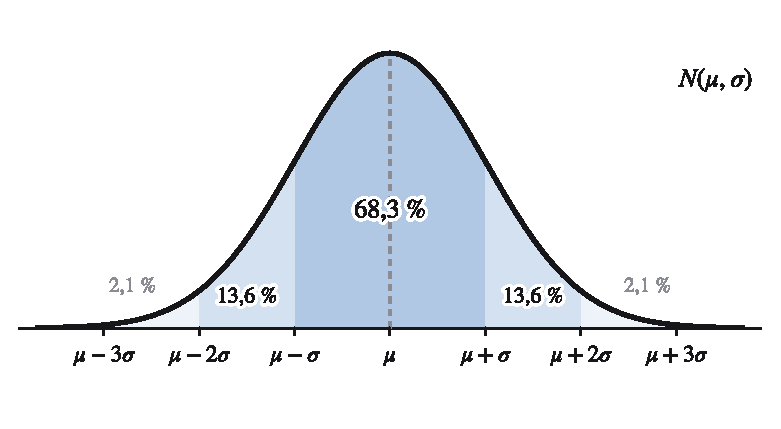
\includegraphics[width=372pt]{fig/m12_f26.pdf}
\caption{Campana de Gauss $N(\mu, \sigma)$: el 68,3 \% de les dades cau dins de $\mu \pm \sigma$, el 95,5 \% dins de $\mu \pm 2\sigma$ i el 99,7 \% dins de $\mu \pm 3\sigma$.}
\end{figure}

\subsection{Propietats de la distribució normal}

\begin{itemize}
\item La corba és simètrica respecte de $x = \mu$.
\item El punt de màxim és $x = \mu$, amb $f(\mu) = \dfrac{1}{\sigma\sqrt{2\pi}}$.
\item Els punts d'inflexió són $x = \mu \pm \sigma$.
\item $P(\mu - \sigma \le X \le \mu + \sigma) \approx 0{,}683$ \emph{(regla 68-95-99,7)}
\item $P(\mu - 2\sigma \le X \le \mu + 2\sigma) \approx 0{,}955$
\item $P(\mu - 3\sigma \le X \le \mu + 3\sigma) \approx 0{,}997$
\end{itemize}

\subsection{Tipificació: la normal estàndard $N(0, 1)$}

Per calcular probabilitats d'una $N(\mu, \sigma)$ qualsevol, es transforma en la normal estàndard $Z \sim N(0, 1)$ mitjançant el canvi de variable:

\begin{equation*}
Z = \frac{X - \mu}{\sigma}
\end{equation*}

\begin{equation*}
P(X \le x) = P\!\left(Z \le \frac{x - \mu}{\sigma}\right) = \Phi\!\left(\frac{x - \mu}{\sigma}\right)
\end{equation*}

on $\Phi(z)$ és la funció de distribució acumulada de la normal estàndard, consultable en taules.

\textbf{Propietat (Simetria de $\Phi$):} per a la normal estàndard es compleix

\begin{equation}
P(Z \le -z) = 1 - P(Z \le z) = 1 - \Phi(z)
\end{equation}

\begin{equation}
P(Z \ge z) = 1 - \Phi(z)
\end{equation}

\begin{equation}
P(a \le Z \le b) = \Phi(b) - \Phi(a)
\end{equation}

\subsection{Aproximació binomial--normal}

Quan $n$ és gran i $p$ no és molt proper a $0$ ni a $1$, la distribució $B(n, p)$ s'aproxima a:

\begin{equation*}
X \sim B(n, p) \approx N(\mu, \sigma) \quad\text{amb}\quad \mu = np, \quad \sigma = \sqrt{npq}
\end{equation*}

\emph{Regla pràctica:} aplicar quan $np \ge 5$ i $nq \ge 5$.

\section{Complement: probabilitat bàsica, taules i arbres}

\subsection{Regla de Laplace i operacions amb successos}

Si tots els resultats són \textbf{equiprobables}:

\begin{equation*}
P(A)=\frac{\text{casos favorables}}{\text{casos possibles}}
\end{equation*}

\begin{table}[H]
\centering
\renewcommand{\arraystretch}{1.25}
\begin{tabular}{lc}
\toprule
Operació & Fórmula \\
\midrule
Contrari & $P(\overline A)=1-P(A)$ \\
Unió & $P(A\cup B)=P(A)+P(B)-P(A\cap B)$ \\
Intersecció (producte) & $P(A\cap B)=P(A)\,P(B\mid A)$ \\
Independents & $P(A\cap B)=P(A)\,P(B)$ \\
Lleis de De Morgan & $P(\overline{A\cup B})=P(\overline A\cap\overline B)$, $\ P(\overline{A\cap B})=P(\overline A\cup\overline B)$ \\
\bottomrule
\end{tabular}
\end{table}

\begin{figure}[H]
\centering
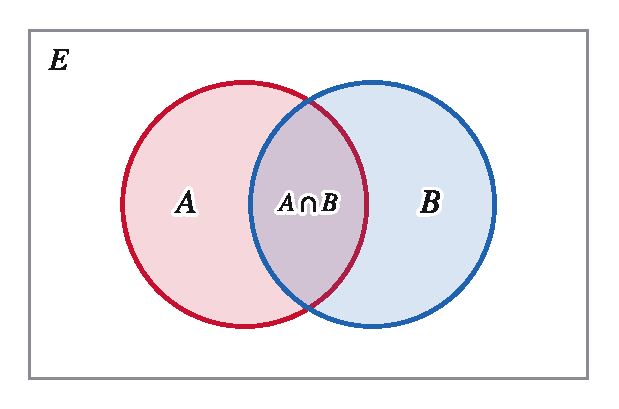
\includegraphics[width=297pt]{fig/m12_f38.pdf}
\caption{Diagrama de Venn de dos successos $A$ i $B$ dins de l'espai mostral $E$.}
\end{figure}

\emph{Exemple:} $P(A)=0{,}5$, $P(B)=0{,}4$ i $P(A\cup B)=0{,}7$. Llavors $P(A\cap B)=0{,}5+0{,}4-0{,}7=0{,}2$. Com que $P(A)P(B)=0{,}2$, \textbf{$A$ i $B$ són independents}.

\subsection{Taules de contingència}

Una taula de doble entrada permet llegir directament les probabilitats.

\begin{table}[H]
\centering
\renewcommand{\arraystretch}{1.25}
\begin{tabular}{lccc}
\toprule
 & $B$ & $\overline B$ & Total \\
\midrule
$A$ & 30 & 20 & 50 \\
$\overline A$ & 10 & 40 & 50 \\
Total & 40 & 60 & 100 \\
\bottomrule
\end{tabular}
\end{table}

$P(A\cap B)=\frac{30}{100}$, $P(B)=\frac{40}{100}$ i $P(A\mid B)=\dfrac{30}{40}=0{,}75$ (es divideix per la fila o columna de la condició).

\subsection{Diagrames d'arbre, probabilitat total i Bayes}

Les probabilitats de les branques d'una mateixa ramificació sumen $1$. El producte de les branques d'un camí és la probabilitat de la intersecció; sumant camins s'obté la \textbf{probabilitat total}.

\begin{figure}[H]
\centering
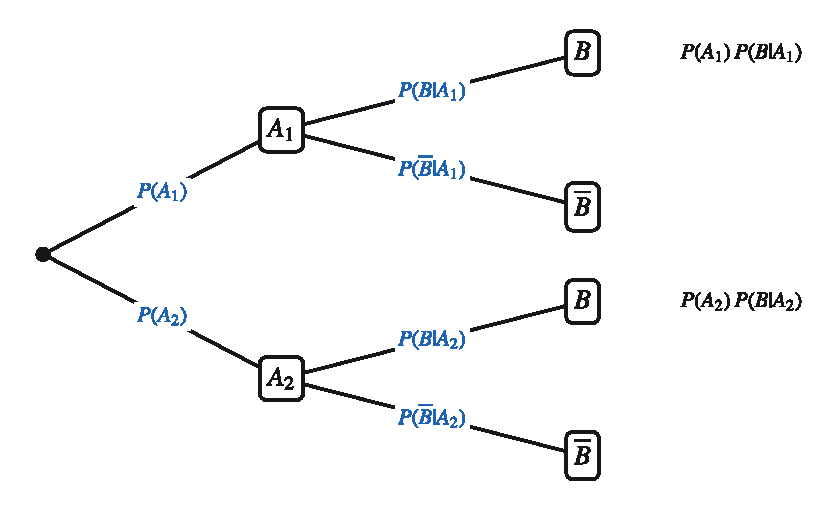
\includegraphics[width=372pt]{fig/m12_f39.pdf}
\caption{Arbre de probabilitats: $P(B)=P(A_1)P(B|A_1)+P(A_2)P(B|A_2)$.}
\end{figure}

\emph{Exemple:} Una fàbrica té dues màquines: $M_1$ fa el $60\,\%$ de les peces, amb un $2\,\%$ de defectuoses, i $M_2$ fa el $40\,\%$, amb un $5\,\%$ de defectuoses.

\begin{equation*}
P(D)=0{,}6\cdot0{,}02+0{,}4\cdot0{,}05=0{,}012+0{,}02=0{,}032
\end{equation*}

Si una peça és defectuosa, la probabilitat que vingui de $M_2$ és (Bayes)

\begin{equation*}
P(M_2\mid D)=\frac{0{,}4\cdot0{,}05}{0{,}032}=\frac{0{,}02}{0{,}032}=0{,}625
\end{equation*}

\section{Complement: esperança, variància i exemples resolts}

\subsection{Esperança i variància}

Per a una variable aleatòria discreta amb valors $x_i$ i probabilitats $p_i$:

\begin{equation*}
\mu=E[X]=\sum x_i\,p_i,\qquad \operatorname{Var}(X)=\sum x_i^2\,p_i-\mu^2,\qquad \sigma=\sqrt{\operatorname{Var}(X)}
\end{equation*}

\emph{Exemple:} Un joc paga $10$ \euro{} amb probabilitat $0{,}1$, $2$ \euro{} amb probabilitat $0{,}4$ i $0$ \euro{} amb probabilitat $0{,}5$.

\begin{equation*}
E[X]=10\cdot0{,}1+2\cdot0{,}4=1{,}8\text{ €},\qquad \operatorname{Var}(X)=100\cdot0{,}1+4\cdot0{,}4-1{,}8^2=11{,}6-3{,}24=8{,}36
\end{equation*}

Per a $B(n,p)$: $E[X]=np$ i $\operatorname{Var}(X)=npq$.

\subsection{Binomial resolta}

Es llança $5$ cops una moneda trucada amb $P(\text{cara})=0{,}6$. Probabilitat d'obtenir \textbf{exactament} $3$ cares i d'obtenir \textbf{almenys} $1$:

\begin{equation*}
P(X=3)=\binom53 0{,}6^3\,0{,}4^2=10\cdot0{,}216\cdot0{,}16=0{,}3456
\end{equation*}

\begin{equation*}
P(X\ge1)=1-P(X=0)=1-0{,}4^5=1-0{,}01024=0{,}98976
\end{equation*}

\subsection{Normal resolta amb tipificació}

Les notes d'un examen segueixen $N(6;\,1{,}5)$. Percentatge d'alumnes amb nota superior a $8$:

\begin{equation*}
P(X>8)=P\!\left(Z>\frac{8-6}{1{,}5}\right)=P(Z>1{,}33)=1-\Phi(1{,}33)=1-0{,}9082=0{,}0918
\end{equation*}

És a dir, un $9{,}18\,\%$ aproximadament. Per a un interval: $P(5\le X\le7)=P(-0{,}67\le Z\le0{,}67)=2\Phi(0{,}67)-1=2\cdot0{,}7486-1=0{,}4972$.

\subsection{Binomial aproximada per la normal}

$X\sim B(100;\,0{,}5)$: $np=50\ge5$, $nq=50\ge5$, de manera que $X\approx N(50;\,5)$ amb $\sigma=\sqrt{100\cdot0{,}5\cdot0{,}5}=5$.

$P(X\le55)$: amb \textbf{correcció de continuïtat} es calcula $P(X'\le55{,}5)$:

\begin{equation*}
P\!\left(Z\le\frac{55{,}5-50}{5}\right)=P(Z\le1{,}1)=\Phi(1{,}1)=0{,}8643
\end{equation*}

% ---------------------------------------------------------------- Annexos
\clearpage\phantomsection\addcontentsline{toc}{bloc}{\protect\numberline{}Annexos}
\newcommand{\annexh}[2]{%
  \stepcounter{temaid}\setcounter{section}{0}\setcounter{equation}{0}
  \phantomsection\addcontentsline{toc}{annex}{\protect\numberline{#1.}#2}
  \begin{center}{\LARGE\bfseries Annex #1: #2}\end{center}\vspace{0.4em}}
\begin{landscape}\annexh{A}{Perímetre, àrea i volum}% Annex A — perímetres, àrees i volums (horitzontal)
\renewcommand{\arraystretch}{2.0}\small
\newcommand{\aT}[2]{\begin{tabular}{@{}p{4.1cm}@{\hspace{0.5em}}c@{\hspace{0.5em}}c@{}}\toprule\textbf{#1}&\textbf{Perímetre}&\textbf{Àrea}\\\midrule #2 \\\bottomrule\end{tabular}}
\begin{minipage}[t]{0.49\linewidth}\centering
\aT{Figura plana}{
Quadrat (costat $l$) & $P=4l$ & $A=l^2$ \\
Rectangle (base $b$, alçada $h$) & $P=2b+2h$ & $A=b\,h$ \\
Paral·lelogram (base $b$, alçada $h$, costat $c$) & $P=2b+2c$ & $A=b\,h$ \\
Rombe (diagonals $D,d$; costat $l$) & $P=4l$ & $A=\D\frac{D\,d}{2}$ \\
Triangle (base $b$, alçada $h$) & $P=a+b+c$ & $A=\D\frac{b\,h}{2}$ \\
Triangle equilàter (costat $l$) & $P=3l$ & $A=\D\frac{\sqrt3}{4}\,l^2$ \\
Trapezi (bases $B,b$; costats $c,d$) & $P=B+b+c+d$ & $A=\D\frac{B+b}{2}\,h$}
\end{minipage}\hfill
\begin{minipage}[t]{0.49\linewidth}\centering
\aT{Figura plana}{
Polígon regular ($n$ costats, apotema $a$) & $P=n\,l$ & $A=\D\frac{P\,a}{2}$ \\
Cercle (radi $r$) & $L=2\pi r$ & $A=\pi r^2$ \\
Sector circular (radi $r$, angle $\theta$ en rad) & $L=\theta\,r$ & $A=\D\frac{\theta\,r^2}{2}$ \\
Corona circular (radis $R>r$) & $2\pi(R+r)$ & $A=\pi(R^2-r^2)$ \\
El·lipse (semieixos $a,b$) & $P\approx 2\pi\sqrt{\D\frac{a^2+b^2}{2}}$ & $A=\pi\,a\,b$ \\
Segment circular (radi $r$, angle $\theta$) & $L=\theta\,r$ & $A=\D\frac{r^2}{2}(\theta-\sin\theta)$ \\
Hexàgon regular (costat $l$) & $P=6l$ & $A=\D\frac{3\sqrt3}{2}\,l^2$}
\end{minipage}
\par\vspace{1.4em}
\renewcommand{\arraystretch}{2.05}
\newcommand{\vT}[2]{\begin{tabular}{@{}p{4.1cm}@{\hspace{0.5em}}c@{\hspace{0.5em}}c@{}}\toprule\textbf{#1}&\textbf{Àrea}&\textbf{Volum}\\\midrule #2 \\\bottomrule\end{tabular}}
\begin{minipage}[t]{0.49\linewidth}\centering
\vT{Cos geomètric}{
Cub (aresta $a$) & $A_T=6a^2$ & $V=a^3$ \\
Ortoedre (arestes $a,b,c$) & $A_T=2(ab+bc+ac)$ & $V=abc$ \\
Prisma (àrea base $A_B$, perímetre $P_B$) & $A_L=P_B\,h;\ A_T=2A_B+A_L$ & $V=A_B\,h$ \\
Piràmide (apotema $a_p$) & $A_L=\D\frac{P_B\,a_p}{2};\ A_T=A_B+A_L$ & $V=\D\frac{A_B\,h}{3}$ \\
Cilindre (radi $r$, alçada $h$) & $A_L=2\pi r h;\ A_T=2\pi r(h+r)$ & $V=\pi r^2h$}
\end{minipage}\hfill
\begin{minipage}[t]{0.49\linewidth}\centering
\vT{Cos geomètric}{
Con (radi $r$, generatriu $g$) & $A_L=\pi r g;\ A_T=\pi r(g+r)$ & $V=\D\frac{\pi r^2h}{3}$ \\
Tronc de con (radis $R,r$) & $A_L=\pi g(R+r)$ & $V=\D\frac{\pi h}{3}(R^2+Rr+r^2)$ \\
Esfera (radi $r$) & $A=4\pi r^2$ & $V=\D\frac{4\pi r^3}{3}$ \\
Semiesfera (radi $r$) & $A_T=3\pi r^2$ & $V=\D\frac{2\pi r^3}{3}$ \\
Calota esfèrica (alçada $h$) & $A=2\pi r h$ & $V=\D\frac{\pi h^2}{3}(3r-h)$}
\end{minipage}
\par\vspace{1.6em}
\renewcommand{\arraystretch}{1.5}\normalsize
\begin{minipage}[t]{0.32\linewidth}
\textbf{Teorema de Pitàgores}\par (triangle rectangle de catets $a,b$ i hipotenusa $c$):
\[c^2=a^2+b^2\]
\[c=\sqrt{a^2+b^2},\qquad a=\sqrt{c^2-b^2}\]
\end{minipage}\hfill
\begin{minipage}[t]{0.32\linewidth}
\textbf{Raons trigonomètriques}\par (triangle rectangle, angle $\alpha$):
\[\sin\alpha=\frac{\text{oposat}}{\text{hipotenusa}},\ \ \cos\alpha=\frac{\text{adjacent}}{\text{hipotenusa}}\]
\[\tan\alpha=\frac{\text{oposat}}{\text{adjacent}},\qquad \sin^2\alpha+\cos^2\alpha=1\]
\end{minipage}\hfill
\begin{minipage}[t]{0.32\linewidth}
\textbf{Fórmula de Heró}\par (semiperímetre $s=\frac{a+b+c}{2}$):
\[A=\sqrt{s(s-a)(s-b)(s-c)}\]
\textbf{Àrea d'un triangle amb dos costats:}
\[A=\tfrac12\,a\,b\,\sin\gamma\]
\end{minipage}
\normalsize
\end{landscape}
\begin{landscape}\annexh{B}{Símbols i notació matemàtica}% Annex B — símbols i notació (horitzontal)
\normalsize\renewcommand{\arraystretch}{1.55}
\newcommand{\sym}[1]{\begin{tabular}{@{}p{2.6cm}p{5.6cm}@{\hspace{2em}}p{2.6cm}p{5.6cm}@{}}\toprule\textbf{Símbol}&\textbf{Significat}&\textbf{Símbol}&\textbf{Significat}\\\midrule #1 \\\bottomrule\end{tabular}}
\needspace{11\baselineskip}\textbf{Símbols generals i d'operació}\par\vspace{2pt}
\sym{
$=$ & igual & $\neq$ & distint \\
$<$ & menor que & $>$ & major que \\
$\le$ & menor o igual que & $\ge$ & major o igual que \\
$\approx$ & aproximadament igual & $\equiv$ & idènticament igual \\
$\propto$ & proporcional a & $\pm,\ \mp$ & més-menys / menys-més \\
$\infty$ & infinit & $\%,\ \text{\textperthousand}$ & tant per cent / per mil \\
$\sum_{i=1}^{n}$ & sumatori & $\prod_{i=1}^{n}$ & productori \\
$|x|$ & valor absolut & $\sqrt[n]{x}$ & arrel $n$-èsima \\
$n!$ & factorial & $a:b,\ \frac ab$ & raó, quocient}
\vspace{0.8em}

\needspace{11\baselineskip}\textbf{Lògica i raonament}\par\vspace{2pt}
\sym{
$\forall$ & per a tot (quantificador universal) & $\exists$ & existeix (quantificador existencial) \\
$\Rightarrow$ & implica (si \dots\ llavors) & $\Leftrightarrow$ & equival (si i només si) \\
$\therefore$ & per tant, per conseqüent & $\because$ & perquè, ja que \\
$\neg$ & negació & $\wedge$ & conjunció (``i'') \\
$\vee$ & disjunció (``o'') & $\mid,\ :$ & tal que \\
$\blacksquare$ & fi de la demostració & $\Longrightarrow$ & implicació forta}
\needspace{11\baselineskip}\textbf{Conjunts i nombres}\par\vspace{2pt}
\sym{
$\mathbb{N}$ & nombres naturals & $\mathbb{Z}$ & nombres enters \\
$\mathbb{Q}$ & nombres racionals & $\mathbb{R}$ & nombres reals \\
$\mathbb{C}$ & nombres complexos & $\mathbb{R}^{+}$ & reals positius \\
$\{a,b,\dots\}$ & conjunt d'elements $a,b,\dots$ & $\emptyset$ & conjunt buit \\
$A\cap B$ & intersecció & $A\cup B$ & unió \\
$A\subset B$ & inclòs en (estricte) & $A\subseteq B$ & inclòs o igual \\
$a\in A$ & $a$ pertany a $A$ & $a\notin A$ & $a$ no pertany a $A$ \\
$A\setminus B$ & diferència de conjunts & $\mathcal P(A)$ & conjunt de parts de $A$ \\
$A^{c},\ \overline A$ & complementari de $A$ & $|A|,\ n(A)$ & cardinal de $A$ \\
$A\times B$ & producte cartesià & $\{x\mid P(x)\}$ & els $x$ tals que $P(x)$ és cert}
\vspace{0.8em}

\needspace{11\baselineskip}\textbf{Intervals}\par\vspace{2pt}
\sym{
$(a,b)$ & interval obert & $[a,b]$ & interval tancat \\
$[a,b)$ & semiobert per la dreta & $(a,b]$ & semiobert per l'esquerra \\
$(a,+\infty)$ & semirecta oberta & $[a,+\infty)$ & semirecta tancada \\
$(-\infty,b)$ & semirecta oberta a l'esquerra & $(-\infty,+\infty)=\mathbb R$ & recta real}
\vspace{0.8em}

\needspace{11\baselineskip}\textbf{Constants i funcions elementals}\par\vspace{2pt}
\sym{
$\pi\approx 3{,}14159$ & nombre pi & $e\approx 2{,}71828$ & nombre d'Euler \\
$\varphi\approx 1{,}61803$ & nombre auri & $\sqrt 2\approx 1{,}41421$ & arrel de dos \\
$\log x$ & logaritme decimal (base 10) & $\log_a x$ & logaritme en base $a$ \\
$\ln x$ & logaritme neperià (base $e$) & $e^{x},\ \exp x$ & exponencial \\
$\sin,\cos,\tan$ & sinus, cosinus, tangent & $\cot,\sec,\csc$ & cotangent, secant, cosecant \\
$\arcsin,\arccos,\arctan$ & funcions trigonomètriques inverses & $\sinh,\cosh,\tanh$ & funcions hiperbòliques}
\needspace{11\baselineskip}\textbf{Càlcul infinitesimal i estadística}\par\vspace{2pt}
\sym{
$\lim_{x\to a}f(x)$ & límit de $f$ quan $x$ tendeix a $a$ & $\Delta x$ & increment de $x$ \\
$f'(x),\ \frac{df}{dx}$ & derivada primera de $f$ & $f''(x),\ \frac{d^2f}{dx^2}$ & derivada segona \\
$f^{(n)}(x)$ & derivada $n$-èsima & $F(x),\ \int f\,dx$ & primitiva, integral indefinida \\
$\int_a^b f\,dx$ & integral definida entre $a$ i $b$ & $[F(x)]_a^b$ & $F(b)-F(a)$ (Barrow) \\
$\bar x,\ \mu$ & mitjana & $\sigma,\ \sigma^2,\ \mathrm{Var}$ & desviació típica, variància \\
$\binom nk$ & nombre combinatori & $C_n^k,\ V_n^k,\ P_n$ & combinacions, variacions, permutacions \\
$P(A),\ P(B\mid A)$ & probabilitat, probabilitat condicionada & $E(X),\ \mu$ & esperança (valor esperat) \\
$B(n,p)$ & distribució binomial & $N(\mu,\sigma)$ & distribució normal \\
$Z=\frac{X-\mu}{\sigma}$ & variable tipificada & $\Phi(z)$ & funció de distribució de $N(0,1)$}
\vspace{0.8em}

\needspace{11\baselineskip}\textbf{Geometria i àlgebra lineal}\par\vspace{2pt}
\sym{
$\overrightarrow{AB}$ & vector d'origen $A$ i extrem $B$ & $|\vec v|$ & mòdul del vector \\
$\vec u\cdot\vec v$ & producte escalar & $\vec u\times\vec v$ & producte vectorial \\
$[\vec u,\vec v,\vec w]$ & producte mixt & $\hat u$ & vector unitari \\
$\parallel$ & paral·lel & $\perp$ & perpendicular \\
$\angle(r,s)$ & angle entre dues rectes & $d(P,Q)$ & distància entre dos punts \\
$d(P,r),\ d(P,\pi)$ & distància d'un punt a una recta, a un pla & $\pi$ & pla \\
$A^{t}$ & matriu transposada & $A^{-1}$ & matriu inversa \\
$|A|,\ \det A$ & determinant de $A$ & $\mathrm{Rg}(A)$ & rang de $A$ \\
$A^{*}$ & matriu ampliada & $I$ & matriu identitat \\
$\mathrm{Adj}(A)$ & matriu d'adjunts & S.C.D./S.C.I./S.I. & sistema comp. determinat/indeterminat/incompatible}
\normalsize
\end{landscape}
\begin{landscape}\annexh{C}{Formulari: límits, derivades i integrals}% Annex C — formulari: límits, derivades, integrals (vertical)
\newcommand{\ft}[3]{\begin{tabular}{@{}l@{\hspace{0.8em}}l@{\hspace{3.2em}}l@{\hspace{0.8em}}l@{}}\toprule\textbf{#1}&\textbf{#2}&\textbf{#1}&\textbf{#2}\\\midrule #3 \\\bottomrule\end{tabular}}
\newcommand{\sub}[1]{\par\vspace{0.9em}{\bfseries #1}\par\vspace{3pt}}
\small\renewcommand{\arraystretch}{1.6}
\begin{center}{\large\bfseries Taula de límits}\end{center}\vspace{-2pt}
\ft{Límit}{Resultat}{
$\lim\limits_{x\to a}k$ & $k$ & $\lim\limits_{x\to+\infty}e^{x}$ & $+\infty$ \\
$\lim\limits_{x\to a}x^{n}$ & $a^{n}$ & $\lim\limits_{x\to-\infty}e^{x}$ & $0$ \\
$\lim\limits_{x\to a}\sqrt[n]{x}$ & $\sqrt[n]{a}$ & $\lim\limits_{x\to+\infty}a^{x}$ & $+\infty\ (a>1),\ 0\ (0<a<1)$ \\
$\lim\limits_{x\to a}e^{x}$ & $e^{a}$ & $\lim\limits_{x\to+\infty}\ln x$ & $+\infty$ \\
$\lim\limits_{x\to a}\ln x$ & $\ln a\ (a>0)$ & $\lim\limits_{x\to0^{+}}\ln x$ & $-\infty$ \\
$\lim\limits_{x\to a}\sin x$ & $\sin a$ & $\lim\limits_{x\to\pm\infty}\D\frac{1}{x^{n}}$ & $0\ (n>0)$ \\
$\lim\limits_{x\to a}\cos x$ & $\cos a$ & $\lim\limits_{x\to+\infty}\arctan x$ & $\D\frac{\pi}{2}$ \\
$\lim\limits_{x\to a}\arctan x$ & $\arctan a$ & $\lim\limits_{x\to-\infty}\arctan x$ & $-\D\frac{\pi}{2}$}
\sub{Límits notables}
\ft{Límit}{Resultat}{
$\lim\limits_{x\to0}\D\frac{\sin x}{x}$ & $1$ & $\lim\limits_{x\to0}\D\frac{e^{x}-1}{x}$ & $1$ \\
$\lim\limits_{x\to0}\D\frac{\tan x}{x}$ & $1$ & $\lim\limits_{x\to0}\D\frac{a^{x}-1}{x}$ & $\ln a$ \\
$\lim\limits_{x\to0}\D\frac{\arcsin x}{x}$ & $1$ & $\lim\limits_{x\to0}\D\frac{\ln(1+x)}{x}$ & $1$ \\
$\lim\limits_{x\to0}\D\frac{\arctan x}{x}$ & $1$ & $\lim\limits_{x\to0}\D\frac{(1+x)^{a}-1}{x}$ & $a$ \\
$\lim\limits_{x\to0}\D\frac{1-\cos x}{x^{2}}$ & $\D\frac12$ & $\lim\limits_{x\to0}(1+x)^{1/x}$ & $e$ \\
$\lim\limits_{x\to0}\D\frac{\sinh x}{x}$ & $1$ & $\lim\limits_{x\to\infty}\Bigl(1+\D\frac{k}{x}\Bigr)^{x}$ & $e^{k}$}
\newpage
\sub{Operacions amb límits \normalfont($\lim f=L,\ \lim g=M$)}
\begin{tabular}{@{}l@{\hspace{0.8em}}l@{\hspace{2.2em}}l@{\hspace{0.8em}}l@{}}\toprule
$\lim(k\,f)$ & $k\,L$ & $\lim\D\frac fg$ & $\D\frac LM\ (M\ne0)$ \\
$\lim(f\pm g)$ & $L\pm M$ & $\lim f^{g}$ & $L^{M}\ (L>0)$ \\
$\lim(f\cdot g)$ & $L\cdot M$ & $\lim\ln f$ & $\ln L\ (L>0)$ \\\bottomrule\end{tabular}
\sub{Operacions amb infinit}
\begin{tabular}{@{}l@{\hspace{0.8em}}l@{\hspace{2.2em}}l@{\hspace{0.8em}}l@{}}\toprule
$\infty+\infty$ & $\infty$ & $\infty\cdot\infty$ & $\infty$ \\
$k\pm\infty$ & $\pm\infty$ & $k\cdot(\pm\infty)$ & $\pm\infty\ (k>0)$ \\
$\D\frac{k}{\pm\infty}$ & $0$ & $\D\frac{k}{0}$ & $\infty\ (k\ne0)$ \\
$(+\infty)^{k}$ & $+\infty\ (k>0),\ 0\ (k<0)$ & $k^{+\infty}$ & $+\infty\ (k>1),\ 0\ (0<k<1)$ \\\bottomrule\end{tabular}
\sub{Ordre de creixement per a $x\to+\infty$}
\[\ln x\ \ll\ x^{n}\ \ll\ a^{x}\ \ll\ x!\ \ll\ x^{x}\qquad(n>0,\ a>1)\]

\sub{Indeterminacions i com resoldre-les}
\begin{tabular}{@{}l@{\hspace{1.2em}}l@{}}\toprule
$\D\frac00$ & factoritzar, multiplicar pel conjugat; Hôpital \\
$\D\frac\infty\infty$ & dividir per la potència més alta; comparar ordres; Hôpital \\
$\infty-\infty$ & denominador comú; multiplicar i dividir pel conjugat \\
$0\cdot\infty$ & passar a $\D\frac{0}{0}$ o $\D\frac\infty\infty$ \\
$1^{\infty}$ & $\D e^{\lim g\,(f-1)}$ \\
$\infty^{0},\ 0^{0}$ & prendre logaritmes: $\ln L=\lim g\ln f$ \\\bottomrule\end{tabular}
\sub{Asímptotes i continuïtat}
\begin{tabular}{@{}l@{\hspace{1.2em}}l@{}}\toprule
Vertical $x=a$ & $\lim\limits_{x\to a^{\pm}}f(x)=\pm\infty$ \\
Horitzontal $y=b$ & $\lim\limits_{x\to\pm\infty}f(x)=b$ \\
Obliqua $y=mx+n$ & $m=\lim\limits_{x\to\pm\infty}\D\frac{f(x)}{x}\neq0,\ \ n=\lim\limits_{x\to\pm\infty}\bigl(f(x)-mx\bigr)$ \\
Contínua en $x=a$ & $\lim\limits_{x\to a}f(x)=f(a)$ \\
Regla de l'Hôpital & $\lim\limits_{x\to a}\D\frac{f}{g}=\lim\limits_{x\to a}\D\frac{f'}{g'}$ (si $\frac00$ o $\frac\infty\infty$) \\\bottomrule\end{tabular}
\sub{Quocients de polinomis per a $x\to\pm\infty$}
\[\lim\limits_{x\to\infty}\D\frac{P(x)}{Q(x)}=\begin{cases}0 & \text{si } \operatorname{gr}P<\operatorname{gr}Q\\[2pt] \D\frac{a_n}{b_n} & \text{si } \operatorname{gr}P=\operatorname{gr}Q\\[2pt] \pm\infty & \text{si } \operatorname{gr}P>\operatorname{gr}Q\end{cases}\]

\newpage
\begin{center}{\large\bfseries Taula de derivades}\ {\small($u=u(x)$; $u'=\frac{du}{dx}$)}\end{center}\vspace{-2pt}
\ft{Funció}{Derivada}{
$k$ & $0$ & $\arctan u$ & $\D\frac{u'}{1+u^{2}}$ \\
$a\,x$ & $a$ & $\arcsin u$ & $\D\frac{u'}{\sqrt{1-u^{2}}}$ \\
$u^{n}$ & $n\,u^{n-1}u'$ & $\arccos u$ & $-\D\frac{u'}{\sqrt{1-u^{2}}}$ \\
$\sqrt{u}$ & $\D\frac{u'}{2\sqrt{u}}$ & $\operatorname{arcsec}u$ & $\D\frac{u'}{|u|\sqrt{u^{2}-1}}$ \\
$\sqrt[n]{u}$ & $\D\frac{u'}{n\sqrt[n]{u^{\,n-1}}}$ & $\operatorname{arccosec}u$ & $-\D\frac{u'}{|u|\sqrt{u^{2}-1}}$ \\
$e^{u}$ & $e^{u}u'$ & $\operatorname{arccotg}u$ & $-\D\frac{u'}{1+u^{2}}$ \\
$a^{u}$ & $a^{u}\ln a\;u'$ & $\sinh u$ & $\cosh u\;u'$ \\
$\ln u$ & $\D\frac{u'}{u}$ & $\cosh u$ & $\sinh u\;u'$ \\
$\log_a u$ & $\D\frac{u'}{u\ln a}$ & $\tanh u$ & $\D\frac{u'}{\cosh^{2}u}$ \\
$\sin u$ & $\cos u\;u'$ & $\operatorname{coth}u$ & $-\D\frac{u'}{\sinh^{2}u}$ \\
$\cos u$ & $-\sin u\;u'$ & $\operatorname{argsinh}u$ & $\D\frac{u'}{\sqrt{u^{2}+1}}$ \\
$\tan u$ & $\D\frac{u'}{\cos^{2}u}=(1+\tan^{2}u)\,u'$ & $\operatorname{argcosh}u$ & $\D\frac{u'}{\sqrt{u^{2}-1}}$ \\
$\cot u$ & $-\D\frac{u'}{\sin^{2}u}$ & $\operatorname{argtanh}u$ & $\D\frac{u'}{1-u^{2}}\ (|u|<1)$ \\
$\sec u$ & $\D\frac{u'\sin u}{\cos^{2}u}$ & $\operatorname{sech}u$ & $-\operatorname{sech}u\tanh u\;u'$ \\
$\csc u$ & $-\D\frac{u'\cos u}{\sin^{2}u}$ & $\operatorname{cosech}u$ & $-\operatorname{cosech}u\coth u\;u'$}
\newpage
\sub{Operacions amb derivades}
\begin{tabular}{@{}l@{\hspace{0.8em}}l@{\hspace{2.2em}}l@{\hspace{0.8em}}l@{}}\toprule
$(k\,u)'$ & $k\,u'$ & $(u\cdot v)'$ & $u'v+uv'$ \\
$(u\pm v)'$ & $u'\pm v'$ & $\Bigl(\D\frac uv\Bigr)'$ & $\D\frac{u'v-uv'}{v^{2}}$ \\
$(u+v-w)'$ & $u'+v'-w'$ & $(u^{v})'$ & $u^{v}\Bigl(v'\ln u+\D\frac{v\,u'}{u}\Bigr)$ \\
$(f\circ g)'(x)$ & $f'(g(x))\cdot g'(x)$ & $(f^{-1})'(y)$ & $\D\frac{1}{f'(x)},\ y=f(x)$ \\\bottomrule\end{tabular}
\sub{Altres tècniques de derivació}
\begin{tabular}{@{}l@{\hspace{1.2em}}l@{}}\toprule
Implícita $F(x,y)=0$ & $y'=-\D\frac{F_x}{F_y}$ \\
Paramètriques $x(t),\,y(t)$ & $\D\frac{dy}{dx}=\D\frac{y'(t)}{x'(t)}$ \\
Logarítmica $y=f(x)^{g(x)}$ & $\ln y=g\ln f\ \Rightarrow\ \D\frac{y'}{y}=(g\ln f)'$ \\
Derivades successives & $f''=(f')',\ \ f^{(n)}=\bigl(f^{(n-1)}\bigr)'$ \\\bottomrule\end{tabular}

\sub{Aplicacions de la derivada}
\begin{tabular}{@{}l@{\hspace{1.2em}}l@{}}\toprule
Definició & $f'(a)=\lim\limits_{h\to0}\D\frac{f(a+h)-f(a)}{h}$ \\
Recta tangent en $x=a$ & $y-f(a)=f'(a)\,(x-a)$ \\
Recta normal en $x=a$ & $y-f(a)=-\D\frac{1}{f'(a)}\,(x-a)\ \ (f'(a)\neq0)$ \\
Creixement & $f'>0$ creix; $f'<0$ decreix \\
Extrems relatius en $x=c$ & $f'(c)=0$ i $\begin{cases}f''(c)>0&\text{mínim}\\f''(c)<0&\text{màxim}\end{cases}$ \\
Concavitat & $f''>0$ còncava ($\cup$); $f''<0$ convexa ($\cap$) \\
Punt d'inflexió en $x=c$ & $f''(c)=0$ i $f'''(c)\neq0$ \\
Teorema del valor mitjà & $f'(c)=\D\frac{f(b)-f(a)}{b-a}$, $c\in(a,b)$ \\
Teorema de Rolle & $f(a)=f(b)\Rightarrow f'(c)=0$ \\\bottomrule\end{tabular}

\newpage
\begin{center}{\large\bfseries Taula d'integrals immediates}\ {\small($u=u(x)$, $a>0$; a cada primitiva s'ha de sumar $+C$)}\end{center}\vspace{-2pt}
\ft{Funció}{Primitiva}{
$k$ & $F(x)=k\,x$ & $\D\frac{u'}{\sqrt{1-u^{2}}}$ & $F=\arcsin u$ \\
$u^{n}u'\ (n\neq-1)$ & $F=\D\frac{u^{n+1}}{n+1}$ & $\D\frac{u'}{1+u^{2}}$ & $F=\arctan u$ \\
$\D\frac{u'}{u}$ & $F=\ln|u|$ & $\D\frac{u'}{a^{2}+u^{2}}$ & $F=\D\frac1a\arctan\D\frac ua$ \\
$e^{u}u'$ & $F=e^{u}$ & $\D\frac{u'}{\sqrt{u^{2}+1}}$ & $F=\ln\bigl(u+\sqrt{u^{2}+1}\bigr)$ \\
$a^{u}u'$ & $F=\D\frac{a^{u}}{\ln a}$ & $\D\frac{u'}{\sqrt{u^{2}-1}}$ & $F=\ln\bigl|u+\sqrt{u^{2}-1}\bigr|$ \\
$\sin u\;u'$ & $F=-\cos u$ & $\D\frac{u'}{1-u^{2}}$ & $F=\D\frac12\ln\Bigl|\D\frac{1+u}{1-u}\Bigr|$ \\
$\cos u\;u'$ & $F=\sin u$ & $\sinh u\;u'$ & $F=\cosh u$ \\
$\tan u\;u'$ & $F=-\ln|\cos u|$ & $\cosh u\;u'$ & $F=\sinh u$ \\
$\cot u\;u'$ & $F=\ln|\sin u|$ & $\D\frac{u'}{\cosh^{2}u}$ & $F=\tanh u$ \\
$\D\frac{u'}{\cos^{2}u}$ & $F=\tan u$ & $\sec u\;u'$ & $F=\ln|\sec u+\tan u|$ \\
$\D\frac{u'}{\sin^{2}u}$ & $F=-\cot u$ & $\csc u\;u'$ & $F=\ln|\csc u-\cot u|$ \\
$\sec u\tan u\;u'$ & $F=\sec u$ & $\csc u\cot u\;u'$ & $F=-\csc u$}
\newpage
\sub{Operacions i aplicacions de la integral}
\begin{tabular}{@{}l@{\hspace{1.2em}}l@{}}\toprule
Linealitat & $\int(f\pm g)\,dx=\int f\,dx\pm\int g\,dx,\ \ \int k\,f=k\int f$ \\
Barrow & $\int_a^b f(x)\,dx=F(b)-F(a)$ \\
Additivitat & $\int_a^b f=\int_a^c f+\int_c^b f$ \\
Àrea entre corbes & $A=\int_a^b\bigl|f(x)-g(x)\bigr|\,dx$ \\
Volum de revolució (eix $OX$) & $V=\pi\int_a^b\bigl[f(x)\bigr]^{2}dx$ \\
Valor mitjà & $\bar f=\D\frac{1}{b-a}\int_a^b f(x)\,dx$ \\
Teorema fonamental & $\D\frac{d}{dx}\int_a^{x}f(t)\,dt=f(x)$ \\\bottomrule\end{tabular}

\sub{Mètodes d'integració}
\begin{tabular}{@{}l@{\hspace{1.2em}}l@{}}\toprule
Per parts & $\int u\,dv=u\,v-\int v\,du$ \quad (tria $u$ segons ALPES) \\
Canvi de variable & $x=g(t)\Rightarrow\int f(x)\,dx=\int f(g(t))\,g'(t)\,dt$ \\
$\sqrt{a^{2}-x^{2}}$ & $x=a\sin t$ \\
$\sqrt{a^{2}+x^{2}}$ & $x=a\tan t$ \\
$\sqrt{x^{2}-a^{2}}$ & $x=a\sec t$ \\
Fraccions simples & $\D\frac{P(x)}{(x-a)(x-b)}=\D\frac{A}{x-a}+\D\frac{B}{x-b}$ \\
Arrel doble & $\D\frac{P(x)}{(x-a)^{2}}=\D\frac{A}{x-a}+\D\frac{B}{(x-a)^{2}}$ \\
Quadràtic irreductible & $\D\frac{Mx+N}{x^{2}+px+q}$: arctan + logaritme \\\bottomrule\end{tabular}

\vspace{1em}

\textbf{Regla ALPES} per triar $u$ en la integració per parts: \textbf{A}rcs, \textbf{L}ogaritmes, \textbf{P}olinomis, \textbf{E}xponencials, \textbf{S}inus i cosinus (en aquest ordre).
\normalsize
\end{landscape}
\begin{landscape}\annexh{D}{Taula de la distribució normal}% generat per tools/gen_normal.py — no editar a mà
\footnotesize\setlength{\tabcolsep}{2.6pt}\renewcommand{\arraystretch}{1.12}
\begin{center}
\begin{tabular}{@{}r|cccccccccc@{}}
\toprule
$z$ & 0{,}00 & 0{,}01 & 0{,}02 & 0{,}03 & 0{,}04 & 0{,}05 & 0{,}06 & 0{,}07 & 0{,}08 & 0{,}09 \\
\midrule
0{,}0 & 0{,}5000 & 0{,}5040 & 0{,}5080 & 0{,}5120 & 0{,}5160 & 0{,}5199 & 0{,}5239 & 0{,}5279 & 0{,}5319 & 0{,}5359 \\
0{,}1 & 0{,}5398 & 0{,}5438 & 0{,}5478 & 0{,}5517 & 0{,}5557 & 0{,}5596 & 0{,}5636 & 0{,}5675 & 0{,}5714 & 0{,}5753 \\
0{,}2 & 0{,}5793 & 0{,}5832 & 0{,}5871 & 0{,}5910 & 0{,}5948 & 0{,}5987 & 0{,}6026 & 0{,}6064 & 0{,}6103 & 0{,}6141 \\
0{,}3 & 0{,}6179 & 0{,}6217 & 0{,}6255 & 0{,}6293 & 0{,}6331 & 0{,}6368 & 0{,}6406 & 0{,}6443 & 0{,}6480 & 0{,}6517 \\
0{,}4 & 0{,}6554 & 0{,}6591 & 0{,}6628 & 0{,}6664 & 0{,}6700 & 0{,}6736 & 0{,}6772 & 0{,}6808 & 0{,}6844 & 0{,}6879 \\
0{,}5 & 0{,}6915 & 0{,}6950 & 0{,}6985 & 0{,}7019 & 0{,}7054 & 0{,}7088 & 0{,}7123 & 0{,}7157 & 0{,}7190 & 0{,}7224 \\
0{,}6 & 0{,}7257 & 0{,}7291 & 0{,}7324 & 0{,}7357 & 0{,}7389 & 0{,}7422 & 0{,}7454 & 0{,}7486 & 0{,}7517 & 0{,}7549 \\
0{,}7 & 0{,}7580 & 0{,}7611 & 0{,}7642 & 0{,}7673 & 0{,}7704 & 0{,}7734 & 0{,}7764 & 0{,}7794 & 0{,}7823 & 0{,}7852 \\
0{,}8 & 0{,}7881 & 0{,}7910 & 0{,}7939 & 0{,}7967 & 0{,}7995 & 0{,}8023 & 0{,}8051 & 0{,}8078 & 0{,}8106 & 0{,}8133 \\
0{,}9 & 0{,}8159 & 0{,}8186 & 0{,}8212 & 0{,}8238 & 0{,}8264 & 0{,}8289 & 0{,}8315 & 0{,}8340 & 0{,}8365 & 0{,}8389 \\
1{,}0 & 0{,}8413 & 0{,}8438 & 0{,}8461 & 0{,}8485 & 0{,}8508 & 0{,}8531 & 0{,}8554 & 0{,}8577 & 0{,}8599 & 0{,}8621 \\
1{,}1 & 0{,}8643 & 0{,}8665 & 0{,}8686 & 0{,}8708 & 0{,}8729 & 0{,}8749 & 0{,}8770 & 0{,}8790 & 0{,}8810 & 0{,}8830 \\
1{,}2 & 0{,}8849 & 0{,}8869 & 0{,}8888 & 0{,}8907 & 0{,}8925 & 0{,}8944 & 0{,}8962 & 0{,}8980 & 0{,}8997 & 0{,}9015 \\
1{,}3 & 0{,}9032 & 0{,}9049 & 0{,}9066 & 0{,}9082 & 0{,}9099 & 0{,}9115 & 0{,}9131 & 0{,}9147 & 0{,}9162 & 0{,}9177 \\
1{,}4 & 0{,}9192 & 0{,}9207 & 0{,}9222 & 0{,}9236 & 0{,}9251 & 0{,}9265 & 0{,}9279 & 0{,}9292 & 0{,}9306 & 0{,}9319 \\
1{,}5 & 0{,}9332 & 0{,}9345 & 0{,}9357 & 0{,}9370 & 0{,}9382 & 0{,}9394 & 0{,}9406 & 0{,}9418 & 0{,}9429 & 0{,}9441 \\
1{,}6 & 0{,}9452 & 0{,}9463 & 0{,}9474 & 0{,}9484 & 0{,}9495 & 0{,}9505 & 0{,}9515 & 0{,}9525 & 0{,}9535 & 0{,}9545 \\
1{,}7 & 0{,}9554 & 0{,}9564 & 0{,}9573 & 0{,}9582 & 0{,}9591 & 0{,}9599 & 0{,}9608 & 0{,}9616 & 0{,}9625 & 0{,}9633 \\
1{,}8 & 0{,}9641 & 0{,}9649 & 0{,}9656 & 0{,}9664 & 0{,}9671 & 0{,}9678 & 0{,}9686 & 0{,}9693 & 0{,}9699 & 0{,}9706 \\
1{,}9 & 0{,}9713 & 0{,}9719 & 0{,}9726 & 0{,}9732 & 0{,}9738 & 0{,}9744 & 0{,}9750 & 0{,}9756 & 0{,}9761 & 0{,}9767 \\
\bottomrule
\end{tabular}
\hspace{2.2em}
\begin{tabular}{@{}r|cccccccccc@{}}
\toprule
$z$ & 0{,}00 & 0{,}01 & 0{,}02 & 0{,}03 & 0{,}04 & 0{,}05 & 0{,}06 & 0{,}07 & 0{,}08 & 0{,}09 \\
\midrule
2{,}0 & 0{,}9772 & 0{,}9778 & 0{,}9783 & 0{,}9788 & 0{,}9793 & 0{,}9798 & 0{,}9803 & 0{,}9808 & 0{,}9812 & 0{,}9817 \\
2{,}1 & 0{,}9821 & 0{,}9826 & 0{,}9830 & 0{,}9834 & 0{,}9838 & 0{,}9842 & 0{,}9846 & 0{,}9850 & 0{,}9854 & 0{,}9857 \\
2{,}2 & 0{,}9861 & 0{,}9864 & 0{,}9868 & 0{,}9871 & 0{,}9875 & 0{,}9878 & 0{,}9881 & 0{,}9884 & 0{,}9887 & 0{,}9890 \\
2{,}3 & 0{,}9893 & 0{,}9896 & 0{,}9898 & 0{,}9901 & 0{,}9904 & 0{,}9906 & 0{,}9909 & 0{,}9911 & 0{,}9913 & 0{,}9916 \\
2{,}4 & 0{,}9918 & 0{,}9920 & 0{,}9922 & 0{,}9925 & 0{,}9927 & 0{,}9929 & 0{,}9931 & 0{,}9932 & 0{,}9934 & 0{,}9936 \\
2{,}5 & 0{,}9938 & 0{,}9940 & 0{,}9941 & 0{,}9943 & 0{,}9945 & 0{,}9946 & 0{,}9948 & 0{,}9949 & 0{,}9951 & 0{,}9952 \\
2{,}6 & 0{,}9953 & 0{,}9955 & 0{,}9956 & 0{,}9957 & 0{,}9959 & 0{,}9960 & 0{,}9961 & 0{,}9962 & 0{,}9963 & 0{,}9964 \\
2{,}7 & 0{,}9965 & 0{,}9966 & 0{,}9967 & 0{,}9968 & 0{,}9969 & 0{,}9970 & 0{,}9971 & 0{,}9972 & 0{,}9973 & 0{,}9974 \\
2{,}8 & 0{,}9974 & 0{,}9975 & 0{,}9976 & 0{,}9977 & 0{,}9977 & 0{,}9978 & 0{,}9979 & 0{,}9979 & 0{,}9980 & 0{,}9981 \\
2{,}9 & 0{,}9981 & 0{,}9982 & 0{,}9982 & 0{,}9983 & 0{,}9984 & 0{,}9984 & 0{,}9985 & 0{,}9985 & 0{,}9986 & 0{,}9986 \\
3{,}0 & 0{,}9987 & 0{,}9987 & 0{,}9987 & 0{,}9988 & 0{,}9988 & 0{,}9989 & 0{,}9989 & 0{,}9989 & 0{,}9990 & 0{,}9990 \\
3{,}1 & 0{,}9990 & 0{,}9991 & 0{,}9991 & 0{,}9991 & 0{,}9992 & 0{,}9992 & 0{,}9992 & 0{,}9992 & 0{,}9993 & 0{,}9993 \\
3{,}2 & 0{,}9993 & 0{,}9993 & 0{,}9994 & 0{,}9994 & 0{,}9994 & 0{,}9994 & 0{,}9994 & 0{,}9995 & 0{,}9995 & 0{,}9995 \\
3{,}3 & 0{,}9995 & 0{,}9995 & 0{,}9995 & 0{,}9996 & 0{,}9996 & 0{,}9996 & 0{,}9996 & 0{,}9996 & 0{,}9996 & 0{,}9997 \\
3{,}4 & 0{,}9997 & 0{,}9997 & 0{,}9997 & 0{,}9997 & 0{,}9997 & 0{,}9997 & 0{,}9997 & 0{,}9997 & 0{,}9997 & 0{,}9998 \\
3{,}5 & 0{,}9998 & 0{,}9998 & 0{,}9998 & 0{,}9998 & 0{,}9998 & 0{,}9998 & 0{,}9998 & 0{,}9998 & 0{,}9998 & 0{,}9998 \\
3{,}6 & 0{,}9998 & 0{,}9998 & 0{,}9999 & 0{,}9999 & 0{,}9999 & 0{,}9999 & 0{,}9999 & 0{,}9999 & 0{,}9999 & 0{,}9999 \\
3{,}7 & 0{,}9999 & 0{,}9999 & 0{,}9999 & 0{,}9999 & 0{,}9999 & 0{,}9999 & 0{,}9999 & 0{,}9999 & 0{,}9999 & 0{,}9999 \\
3{,}8 & 0{,}9999 & 0{,}9999 & 0{,}9999 & 0{,}9999 & 0{,}9999 & 0{,}9999 & 0{,}9999 & 0{,}9999 & 0{,}9999 & 0{,}9999 \\
3{,}9 & 1{,}0000 & 1{,}0000 & 1{,}0000 & 1{,}0000 & 1{,}0000 & 1{,}0000 & 1{,}0000 & 1{,}0000 & 1{,}0000 & 1{,}0000 \\
\bottomrule
\end{tabular}
\end{center}
\normalsize\vspace{0.4em}
\begin{minipage}[t]{0.52\linewidth}
\textbf{Com s'utilitza.} La taula dona $\Phi(z)=P(Z\le z)$ per a $Z\sim N(0,1)$. Per a $z$ amb dues xifres decimals, es busca la fila de la unitat i el primer decimal i la columna del segon decimal. Per exemple, $\Phi(1{,}37)$ és la intersecció de la fila $1{,}3$ amb la columna $0{,}07$:
\[\Phi(1{,}37)=0{,}9147.\]
Per a valors negatius se simplifica amb la simetria: $\Phi(-z)=1-\Phi(z)$. Si $X\sim N(\mu,\sigma)$, es tipifica $Z=\frac{X-\mu}{\sigma}$ i $P(X\le x)=\Phi\bigl(\frac{x-\mu}{\sigma}\bigr)$.
\end{minipage}\hfill
\begin{minipage}[t]{0.43\linewidth}
\textbf{Valors crítics i regla empírica}\par\vspace{2pt}
\renewcommand{\arraystretch}{1.35}\small
\begin{tabular}{@{}c c c@{\hspace{1.6em}}c c@{}}\toprule
Confiança & $\alpha$ & $z_{\alpha/2}$ & Interval & $P(\mu-k\sigma\le X\le\mu+k\sigma)$ \\\midrule
90\,\% & 0{,}10 & 1{,}645 & $\mu\pm\sigma$ & 68{,}27\,\% \\
95\,\% & 0{,}05 & 1{,}960 & $\mu\pm2\sigma$ & 95{,}45\,\% \\
99\,\% & 0{,}01 & 2{,}576 & $\mu\pm3\sigma$ & 99{,}73\,\% \\
\bottomrule\end{tabular}
\end{minipage}
\end{landscape}
\begin{landscape}\annexh{E}{Gràfiques de funcions elementals}% Annex E — gràfiques de funcions elementals (vertical)
\begin{center}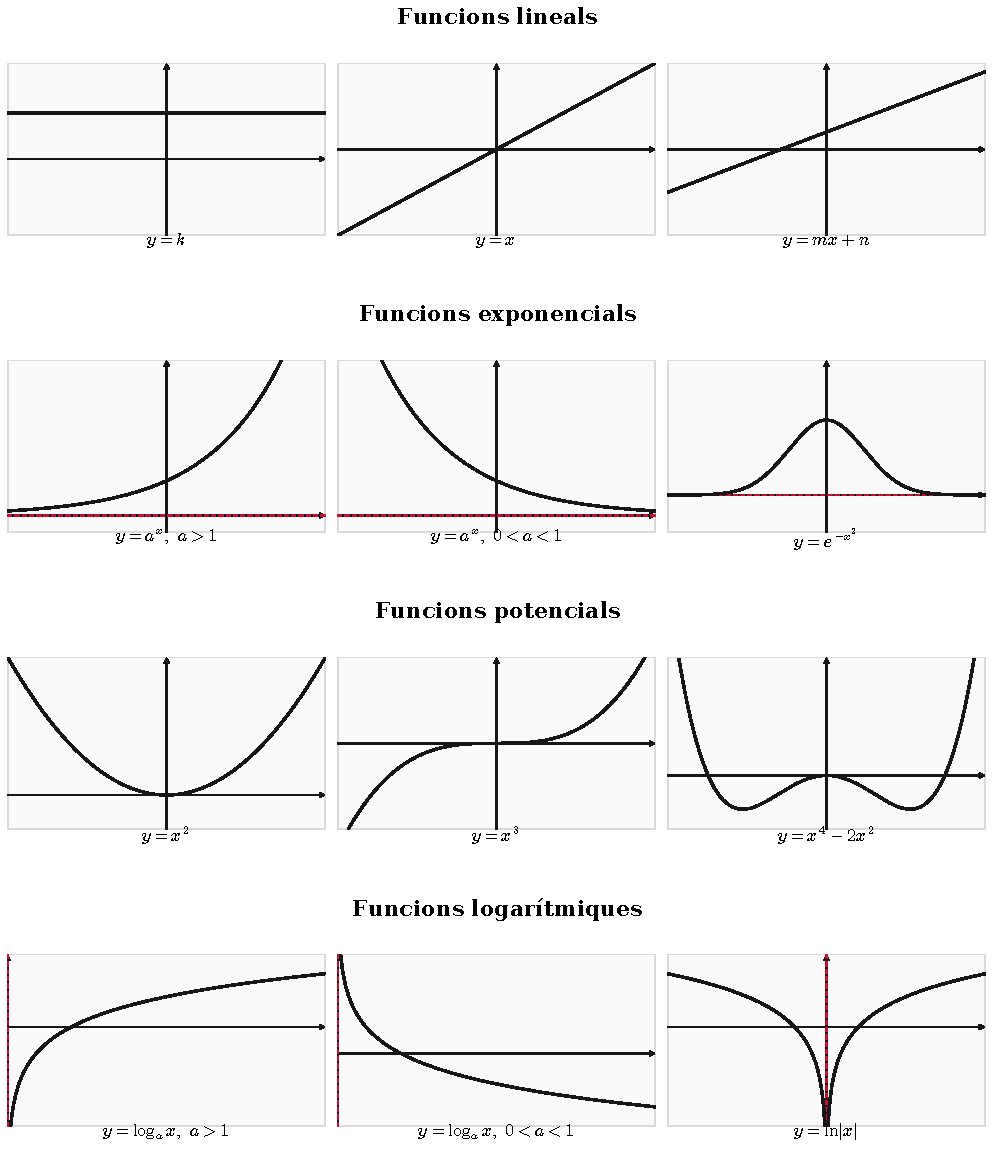
\includegraphics[width=\linewidth,height=0.86\textheight]{fig/x_graphs1.pdf}\end{center}
\clearpage
\begin{center}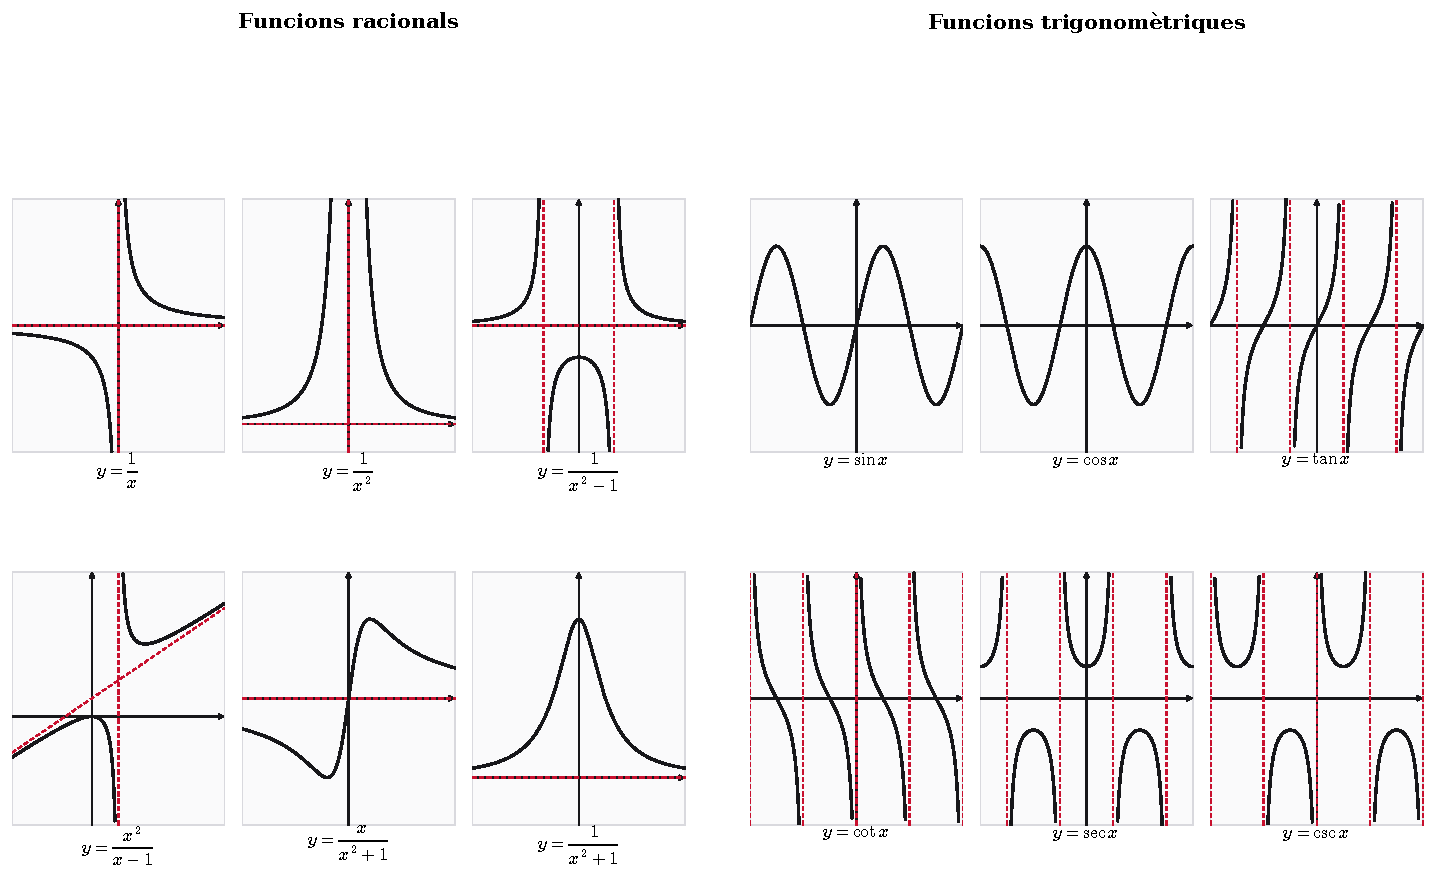
\includegraphics[width=\linewidth,height=0.86\textheight]{fig/x_graphs2.pdf}\end{center}
\clearpage
\begin{center}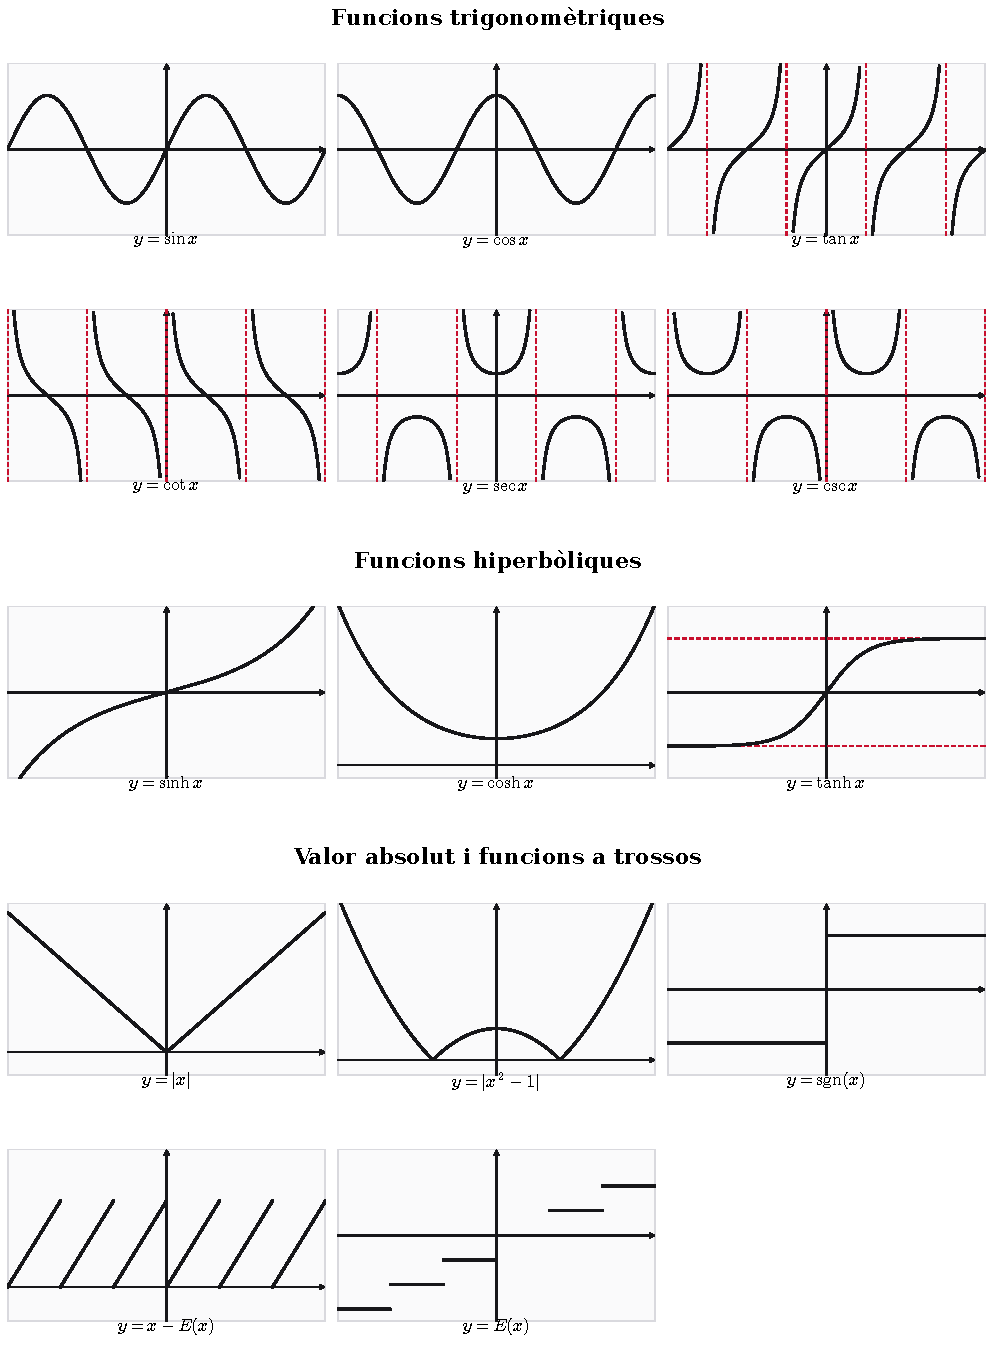
\includegraphics[width=\linewidth,height=0.86\textheight]{fig/x_graphs3.pdf}\end{center}
\end{landscape}
\begin{landscape}\annexh{F}{Fórmules clau per a la PAU}% Annex F — fórmules clau per a la PAU (horitzontal)
\normalsize\renewcommand{\arraystretch}{1.6}
\newcommand{\bx}[2]{\begin{minipage}[t]{0.485\linewidth}{\large\bfseries #1}\par\vspace{3pt}\hrule\vspace{4pt}\begin{itemize}\setlength{\itemsep}{3pt}#2\end{itemize}\end{minipage}}
\bx{Anàlisi}{
\item \textbf{Recta tangent} a $y=f(x)$ en $x=a$: $y-f(a)=f'(a)(x-a)$. \textbf{Normal:} $y-f(a)=-\dfrac{1}{f'(a)}(x-a)$.
\item \textbf{Extrems:} $f'(c)=0$; $f''(c)>0\Rightarrow$ mínim, $f''(c)<0\Rightarrow$ màxim. \textbf{Inflexió:} $f''(c)=0,\ f'''(c)\ne0$.
\item \textbf{Límits notables:} $\lim\limits_{x\to0}\dfrac{\sin x}{x}=1$, \ $\lim\limits_{x\to0}\dfrac{e^x-1}{x}=1$, \ $\lim\limits_{x\to\infty}\bigl(1+\dfrac1x\bigr)^{x}=e$.
\item \textbf{Indeterminació $1^\infty$:} $\lim f^{g}=e^{\lim g\,(f-1)}$. \textbf{Hôpital:} $\lim\dfrac fg=\lim\dfrac{f'}{g'}$.
\item \textbf{Bolzano:} $f$ contínua en $[a,b]$ i $f(a)f(b)<0\Rightarrow\exists c\in(a,b):f(c)=0$.
\item \textbf{Rolle:} $f(a)=f(b)\Rightarrow\exists c:f'(c)=0$. \textbf{Lagrange:} $f'(c)=\dfrac{f(b)-f(a)}{b-a}$.
\item \textbf{Weierstrass:} $f$ contínua en $[a,b]$ té màxim i mínim absoluts en $[a,b]$.
\item \textbf{Barrow:} $\int_a^b f=F(b)-F(a)$. \textbf{Teorema fonamental:} $\dfrac{d}{dx}\int_a^{u(x)}f=f(u(x))\,u'(x)$.
\item \textbf{Àrea entre corbes:} $A=\int_a^b|f-g|\,dx$ (dividint en trams si es creuen). \textbf{Volum de revolució:} $V=\pi\int_a^b f^{2}dx$.
\item \textbf{Per parts:} $\int u\,dv=uv-\int v\,du$ (ALPES). \textbf{Fraccions simples} si $\operatorname{gr}P<\operatorname{gr}Q$.}
\hfill
\bx{Àlgebra}{
\item \textbf{Producte de matrius:} $(AB)_{ij}=\sum_k a_{ik}b_{kj}$; en general $AB\ne BA$. $(AB)^{t}=B^{t}A^{t}$, $(AB)^{-1}=B^{-1}A^{-1}$.
\item \textbf{Determinant $2\times2$:} $\left|\begin{smallmatrix}a&b\\c&d\end{smallmatrix}\right|=ad-bc$. \textbf{Sarrus} per a $3\times3$.
\item \textbf{Propietats:} $|AB|=|A||B|$, $|A^{t}|=|A|$, $|kA|=k^{n}|A|$; fila de zeros $\Rightarrow|A|=0$; dues files iguals o proporcionals $\Rightarrow|A|=0$.
\item \textbf{Inversa:} $A^{-1}=\dfrac{1}{|A|}\bigl(\operatorname{Adj}A\bigr)^{t}$ si $|A|\ne0$ (o per Gauss-Jordan $(A\mid I)\to(I\mid A^{-1})$).
\item \textbf{Equacions matricials:} $AX=B\Rightarrow X=A^{-1}B$; $XA=B\Rightarrow X=BA^{-1}$; $AX+X=B\Rightarrow X=(A+I)^{-1}B$.
\item \textbf{Rouché-Frobenius:} $\operatorname{Rg}A=\operatorname{Rg}A^{*}=n\Rightarrow$ S.C.D.; $\operatorname{Rg}A=\operatorname{Rg}A^{*}<n\Rightarrow$ S.C.I.; $\operatorname{Rg}A<\operatorname{Rg}A^{*}\Rightarrow$ S.I.
\item \textbf{Cramer} (S.C.D.): $x_i=\dfrac{|A_i|}{|A|}$, on $A_i$ té la columna $i$ substituïda pels termes independents.
\item \textbf{Sistemes homogenis:} sempre compatibles; solució no trivial si $|A|=0$.
\item \textbf{Discussió amb paràmetre:} determinant $|A|=0$ $\to$ valors crítics; estudiar $\operatorname{Rg}A$ i $\operatorname{Rg}A^{*}$ per a cadascun.}
\newpage
\bx{Geometria}{
\item \textbf{Vector:} $\overrightarrow{AB}=B-A$; mòdul $|\vec v|=\sqrt{v_1^2+v_2^2+v_3^2}$; unitari $\hat v=\vec v/|\vec v|$; punt mitjà $M=\dfrac{A+B}{2}$.
\item \textbf{Escalar:} $\vec u\cdot\vec v=|\vec u||\vec v|\cos\alpha=u_1v_1+u_2v_2+u_3v_3$; $\cos\alpha=\dfrac{\vec u\cdot\vec v}{|\vec u||\vec v|}$.
\item \textbf{Vectorial:} $|\vec u\times\vec v|=|\vec u||\vec v|\sin\alpha$ = àrea del paral·lelogram; $\vec u\times\vec v\perp\vec u,\vec v$.
\item \textbf{Mixt:} $[\vec u,\vec v,\vec w]=\vec u\cdot(\vec v\times\vec w)$; volum paral·lelepípede $=|[\vec u,\vec v,\vec w]|$; tetraedre $=\dfrac16|[\cdot]|$.
\item \textbf{Recta:} $\dfrac{x-x_0}{v_1}=\dfrac{y-y_0}{v_2}=\dfrac{z-z_0}{v_3}$. \textbf{Pla:} $Ax+By+Cz+D=0$, normal $\vec n=(A,B,C)$.
\item \textbf{Pla per 3 punts:} $\vec n=\overrightarrow{AB}\times\overrightarrow{AC}$. \textbf{Feix de plans:} $\alpha(Ax+By+Cz+D)+\beta(A'x+B'y+C'z+D')=0$.
\item \textbf{Distància punt–pla:} $d(P,\pi)=\dfrac{|Ax_0+By_0+Cz_0+D|}{\sqrt{A^2+B^2+C^2}}$. \textbf{Punt–recta:} $d(P,r)=\dfrac{|\vec u\times\overrightarrow{QP}|}{|\vec u|}$.
\item \textbf{Entre rectes que s'encreuen:} $d(r,s)=\dfrac{|[\vec u,\vec v,\overrightarrow{PQ}]|}{|\vec u\times\vec v|}$.
\item \textbf{Angles:} rectes $\cos\alpha=\dfrac{|\vec u\cdot\vec v|}{|\vec u||\vec v|}$; recta–pla $\sin\alpha=\dfrac{|\vec u\cdot\vec n|}{|\vec u||\vec n|}$; plans $\cos\alpha=\dfrac{|\vec n\cdot\vec n'|}{|\vec n||\vec n'|}$.
\item \textbf{Simètric d'un punt:} respecte d'un punt $M$: $P'=2M-P$; respecte d'un pla/recta: $M$ = projecció ortogonal de $P$, $P'=2M-P$.}
\hfill
\bx{Probabilitat}{
\item \textbf{Laplace:} $P(A)=\dfrac{\text{casos favorables}}{\text{casos possibles}}$. \textbf{Complementari:} $P(A^{c})=1-P(A)$.
\item \textbf{Unió:} $P(A\cup B)=P(A)+P(B)-P(A\cap B)$. \textbf{Lleis de De Morgan:} $\overline{A\cup B}=\overline A\cap\overline B$.
\item \textbf{Condicionada:} $P(B\mid A)=\dfrac{P(A\cap B)}{P(A)}$; \textbf{producte:} $P(A\cap B)=P(A)\,P(B\mid A)$. Independents: $P(A\cap B)=P(A)P(B)$.
\item \textbf{Probabilitat total:} $P(B)=\sum_i P(A_i)\,P(B\mid A_i)$. \textbf{Bayes:} $P(A_i\mid B)=\dfrac{P(A_i)P(B\mid A_i)}{P(B)}$.
\item \textbf{Esperança i variància:} $\mu=\sum x_iP(x_i)$; $\sigma^{2}=\sum x_i^{2}P(x_i)-\mu^{2}$.
\item \textbf{Binomial $B(n,p)$:} $P(X=k)=\binom nk p^{k}q^{\,n-k}$, $q=1-p$; $\mu=np$; $\sigma^{2}=npq$.
\item \textbf{Normal $N(\mu,\sigma)$:} tipificació $Z=\dfrac{X-\mu}{\sigma}\sim N(0,1)$; $P(X\le x)=\Phi\bigl(\dfrac{x-\mu}{\sigma}\bigr)$.
\item \textbf{Simetria:} $\Phi(-z)=1-\Phi(z)$; $P(a\le X\le b)=\Phi(z_b)-\Phi(z_a)$.
\item \textbf{Aproximació binomial--normal:} si $np\ge5$ i $nq\ge5$, $B(n,p)\approx N(np,\sqrt{npq})$ amb correcció de continuïtat ($\pm0{,}5$).
\item \textbf{Regla empírica:} $68{,}3\,\%$, $95{,}4\,\%$, $99{,}7\,\%$ dins de $\mu\pm\sigma,\ \mu\pm2\sigma,\ \mu\pm3\sigma$.}
\normalsize
\end{landscape}
\end{document}
